\documentclass{article}

\usepackage{tabularx}

% https://tex.stackexchange.com/a/129100/125609, to draw the pico ampremeter
\usepackage{tikz}
\usetikzlibrary{arrows}
\usetikzlibrary{shapes}
\newcommand*\circled[1]{\tikz[baseline=(char.base)]{
		            \node[shape=circle,draw,inner sep=1pt] (char) {#1};}}

% NOTE: To put equations in their environment we need either `float` or
% `caption`.  We use float to put equations and other environments exactly
% where they appear in the code with the `H` placeholder, and for that we
% redefine the `equ` environment sort of twice, so this is a bit flaky but
% it works.
\usepackage{caption}
\usepackage{subcaption}

\DeclareCaptionType{equ}[][]
\captionsetup[equ]{name=נוסחא}
\usepackage{float}
\floatstyle{plain}
% https://www.overleaf.com/learn/latex/Positioning_of_Figures
\newfloat{equ}{H}{eq}[section]
\floatname{equ}{נוסחא}

\DeclareCaptionType{graph}[][]
\captionsetup[graph]{name=גרף }

% to includegraphics
\usepackage{graphicx}

% to fix itemize lists:
% https://tex.stackexchange.com/a/53453/125609
\usepackage{enumitem}
\setlist[itemize,1]{label={\fontfamily{cmr}\fontencoding{T1}\selectfont\textbullet}}

% To crop inserted images: https://tex.stackexchange.com/questions/57418/crop-an-inserted-image
\usepackage[export]{adjustbox}

% Links
\usepackage{hyperref}
\hypersetup{colorlinks = true,
	citecolor = gray,
	linkcolor = red,
	citecolor = green,
	filecolor = magenta,
	urlcolor = cyan
}

\usepackage[version=4]{mhchem}

% To include plots by matplotlib
\usepackage{pgf}
\usepackage{pgfplots}
\pgfplotsset{compat=newest}
% Note we use resizebox as explained here through out the document https://tex.stackexchange.com/a/582956/125609

\usepackage{geometry}
 \geometry{
 a4paper,
 top=30mm,
 left = 25mm,
 right = 25mm,
 bottom=30mm,
 headheight=2cm,
 headsep=2cm,
 footskip=1.5cm
}

% Language
\usepackage{polyglossia}
\setdefaultlanguage{hebrew}
\setotherlanguage{english}
\usepackage{hebrewcal}

\usepackage[
backend=biber,
isbn=false,
style=numeric,
doi = false,
sorting=ynt
]{biblatex}
% Seems to be a recommended package but it makes quotes in bibliography at the
% end appear with a question mark instead of `"`.
%\usepackage{csquotes}
\addbibresource{references.bib} % Imports bibliography file

% Fonts
\setmainfont{David CLM}
\setsansfont{Libertinus Serif}
\setmonofont{FreeMono}
\newfontfamily\hebrewfont{David CLM}[Script=Hebrew]
\newfontfamily\hebrewfontsf{Libertinus Serif}[Script=Hebrew]
\newfontfamily\hebrewfonttt{FreeMono}[Script=Hebrew]

\title{

} 
\author{
שרה לחצר ודורון בכר \\
הפקולטה לפיזיקה, טכניון - מכון טכנולוגי לישראל.
}
\date{\today}

\begin{document}
\maketitle

\begin{abstract}
תקציר

של

חמש

שורות

אולי 

שש


\end{abstract}

\section{מבוא}
\subsection{מדידת קבוע סליל בשיטת ESR}
בניסוי זה השתמשנו בשיטת סחריר האלקטרון, שיטה בה חוקרים תכונות של חומרים בעלי אלקטרונים לא מזווגים.
בתהודת סחריר האלקטרון 
,\textenglish{ESR},
נמדדת בליעת אנרגיה של אלקטרונים בנוכחות שדה מגנטי חיצוני.

השדה המגנטי גורם לאלקטרונים להסתדר במקביל ובאנטי מקביל ביחס אליו כתלות במומנטים המגנטיים שלהם. כתוצאה מכך, נוצר פיצול ברמות האנרגיה.
בעזרת אפקט זימן, נוכל לקבוע כי ההפרש בין רמות האנרגיה לאחר הפיצול נתון בנוסחא
\ref{equ:U_gap}.

\begin{equ}
$$ \Delta U = g \mu _B H$$
\caption{
הפער האנרגטי בין רמות האנרגיה שנוצרו משדה מגנטי חיצוני-
$H$
עבור אלקטרונים חופשיים ולא מזווגים,
כאשר
$\mu _B$
המגנטון של בוהר-
ו-$g$
קבוע הפיצול
.
}
\label{equ:U_gap}
\end{equ}
פילוג האלקטרונים בשתי רמות האנרגיה יהיה בהתאם להתפלגות בולצמן, כך שהרמה האנרגטית הנמוכה תהיה מאוכלסת יותר מהרמה האנרגית הגבוהה .

לפיכך, בהכנסת פוטונים בעלי אנרגיה 
$\Delta U$
, יעברו יותר אלקטרונים מהרמה התחתונה לעליונה מאשר להיפך, כך שתבלע אנרגיה במערכת.

%TODO: redo this section, check again about T2
\subsection{מדידת זמן רלקסציה $T_2$}
רלקסציה היא החזרה לשיווי משקל של המגנטיזציה לאחר ערעורה, היא מאופיינת ע"י גודל הנקרא זמן רלקסציה.
קיימים שני סוגים של זמני רלקסציה:
$spin-lattice - T_1$
ו-
$spin-spin - T_2$.
במערכת ה
$ESR$
ניתן למדוד את זמן הרלקסציה $T_2$.
זמן זה, מושפע מחוסר הומוגניות של השדה המגנטי ומאינטרקציות ספין ספין הגורמות לחוסר סנכרון בפאזות הספינים.
 
ניתן לחלץ את ערכו של זמן הרלקסיה - 
$T_2$,
מתוך נוסחא
\label{equ:absorptionRate},
בעזרת רוחב הלורנציאן.


\begin{equ}
$$ P(\omega) = \frac{\omega \gamma M_z T_2 H_1^2}{1+ (\omega_0 -\omega)^2 T^2_2} $$
\caption{
קצב בליעת האנרגיה כתלות ב
$M_z$
מגנטציית הדגם,
$T_2$
זמן רלקסציה,
$\gamma = \frac{g \mu_B}{\hbar}$
ותדירות התהודה של המערכת}

\label{equ:absorptionRate}
\end{equ}

\clearpage
\section{מערכת הניסוי}



מערכת הניסוי מורכבת מסליל חיצוני וסליל פנימי בהם מוצב הדגם, כפי שמוצג באיור 
\ref{fig:experiment_scheme}. 
בסליל החיצוני 4 שכבות של 110 ליפופים,
גובהו 
$h = 0.07 m$,
הקוטר הממוצע שלו הוא
$D = 0.04 m$.
נוכל להיעזר בחוק ביו סבר ולפתח ביטוי עבור קבוע הסליל, הביטוי מוצג בנוסחא
\ref{equ:K_theory}.

\begin{equ}
$$k = \mu_0 \frac{N}{\sqrt{h^2 + D^2}}$$
\caption{קבוע הסליל מחושב בעזרת חוק ביו סבר כתלות במספר הליפופים בסליל, גובהו וקוטרו.}
\label{equ:K_theory}
\end{equ}
 
\begin{figure}[ht!]
    \centering
    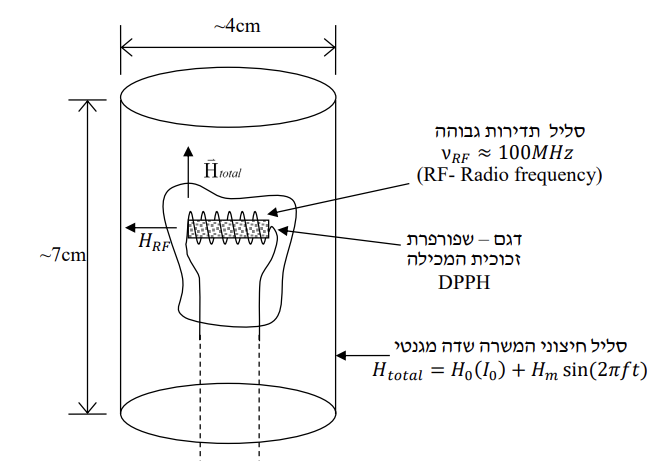
\includegraphics[width=0.7\textwidth]{schematic_setup.png}
    \caption{סכמה של מערכת הניסוי}
    \label{fig:experiment_scheme}
\end{figure}

הזרם הזורם בסליל החיצוני יוצר את השדה המגנטי הגורם לפיצול רמות האנרגיה, ואילו הסליל הפנימי מספק אנרגיה למערכת הגורמת לערור האלקטרונים. 
בניגוד למקובל בספקטרוסקופיה בה משנים את האנרגיה המסופקת למערכת לערעור האלקטרונים, בניסוי זה נשנה את השדה המגנטי החיצוני וכך את רמות האנרגיה.

 
 
 
בסליל החיצוני נזרים זרם חילופין באמפליטודה
$I_m$,
בכדי ליצור פיצול ברמות האנרגיה המשתנה בזמן שיגרום לתהודה באופן מחזורי.
בנוסף נזרים זרם ישר
$I_0$,
כך השדה המגנטי הכולל מוצג בנוסחא
\ref{equ:H_outer_inductor}.
\begin{equ}
$$ H_{total} = k \cdot (I_0 + I_m sin(2 \pi ft))$$
\caption{
השדה המגנטי בסליל החיצוני כתלות בזרמי הסליל, 
תדירות מתח החליפין 
$f$
וקבוע הפרופורציה 
$k$.
}
\label{equ:H_outer_inductor}
\end{equ}

בסליל הקטן מוזרם זרם חילופין היוצר שדה אלקטרומגנטי 
$H_{RF}$
בתדירות קבועה
$v_{RF} = 97.91 \pm 0.02 MHz$.
כאמור במבוא, כאשר השדה בסליל החיצוני יהיה שווה ל
$H_{RF}$
נצפה לקבל בליעה של אנרגיה.

הדגם המוצב במערכת הוא פחמימן מוצק -
\textenglish{DPPH},
המכיל רדיקלים חופשיים בעלי אלקטרונים בלתי מזווגים
שיאפשרו לקבל את אפקט זימן.
הצימוד בין אלקטרונים אלה לבין הסריג האטומי הוא חלש, ולכן ערכו של
$g$
קרוב לאלקטרון חופשי ושווה ל-
$g = 2.0036 \pm 0.0002$.


מדידת בליעת האנרגיה מסתמכת על כך שבעת בליעה מתרחש שינוי בפרמאביליות של הדגם. כיוון שהדגם משמש כליבה של סליל במעגל
$RLC$,
 בבליעה מתרחש שינוי בההשראות ובההתנגדות שלו.
ההתנגדות האפקטיבית של הסליל היא פונקציה של בליעת האנרגיה ע"י הליבה ובמצב תהודה ההתנגדות
במעגל ה
-$RLC$
גדלה וגורמת להגדלת אמפליטודת התנודות, בהסתמך על אפקט זה נוכל למדוד את הבליעה.
\clearpage
\section{מהלך הניסוי ותוצאותיו}
\subsection{מדידת קבוע סליל בשיטת ESR }
בניסוי זה מדדנו בשתי דרכים שונות את קבוע הסליל.


תחילה, קבענו את הזרם הישר ל-
$I_0 = 0$,
וכיוונו את אמפליטודת המודולציה
$I_m$
לעוצמה הגורמת לשדה מגנטי לקיים את משוואה
\ref{equ:U_gap}.
במצב זה מתקבלים פיקים באות הבליעה, במרחקים שווים, ובנקודות הקיצון של אות המודולציה. מדדנו את המערכת במצב זה, ובגרף 
\ref{graph:p2p_measurement}
מוצג אות הבליעה יחד עם אות המודולציה שמדדנו.

סימנו ב-
$\times$
את הנקודות בהן התקבלו בליעות מקסימליות, וביצענו התאמה בין אות המודולציה לאות סינוסואידלי. בעזרת ההתאמה סימנו את המיקומים באות המודולציה בהם התקבלו הפיקים בקו מקווקו.
\textbf{
קיבלנו שהפיקים באות הבליעה ושנקודות הקיצון של אות המודולציה התקבלו באותו הזמן בדיוק, עד כדי תדר הדגימה של משקף התנודות
}.


טיב ההתאמה לאות הסינוסואידלי היה
$R^2 = 1.00$
וערך האמפליטודה היה
$0.521\pm0.002 [A]$.
ערכו של השדה המגנטי ברזוננס לפי נוסחא
\ref{equ:U_gap}
הינו
$34.914\pm0.009 [gauss]$,
כאשר השגיאה של ערך זה נובעת מאי הוודאות של
$g$
ואי הוודאות ב-
$\nu_{RF}$.
מתוך
\ref{equ:H_outer_inductor}
קיבלנו
$k_1 = 66.9\pm 0.3 [\frac{gauss}{A}]$.

הבחנו שקיימת אי-סימטריה סביב הפיקים במדידת הבליעה, הסקנו שהיא נובעת מהזמן שלוקח למערכת להתייצב לאחר הבליעה.
\begin{graph}[H]
	\begin{center}
	\resizebox{\textwidth}{!}{%% Creator: Matplotlib, PGF backend
%%
%% To include the figure in your LaTeX document, write
%%   \input{<filename>.pgf}
%%
%% Make sure the required packages are loaded in your preamble
%%   \usepackage{pgf}
%%
%% Also ensure that all the required font packages are loaded; for instance,
%% the lmodern package is sometimes necessary when using math font.
%%   \usepackage{lmodern}
%%
%% Figures using additional raster images can only be included by \input if
%% they are in the same directory as the main LaTeX file. For loading figures
%% from other directories you can use the `import` package
%%   \usepackage{import}
%%
%% and then include the figures with
%%   \import{<path to file>}{<filename>.pgf}
%%
%% Matplotlib used the following preamble
%%   \usepackage{fontspec}
%%   \setmainfont{DejaVuSerif.ttf}[Path=\detokenize{/nix/store/pzyssb3mfyaisyvpajrr24nhvkm8sk74-python3.9-matplotlib-3.5.1/lib/python3.9/site-packages/matplotlib/mpl-data/fonts/ttf/}]
%%   \setsansfont{DejaVuSans.ttf}[Path=\detokenize{/nix/store/pzyssb3mfyaisyvpajrr24nhvkm8sk74-python3.9-matplotlib-3.5.1/lib/python3.9/site-packages/matplotlib/mpl-data/fonts/ttf/}]
%%   \setmonofont{DejaVuSansMono.ttf}[Path=\detokenize{/nix/store/pzyssb3mfyaisyvpajrr24nhvkm8sk74-python3.9-matplotlib-3.5.1/lib/python3.9/site-packages/matplotlib/mpl-data/fonts/ttf/}]
%%
\begingroup%
\makeatletter%
\begin{pgfpicture}%
\pgfpathrectangle{\pgfpointorigin}{\pgfqpoint{6.400000in}{4.800000in}}%
\pgfusepath{use as bounding box, clip}%
\begin{pgfscope}%
\pgfsetbuttcap%
\pgfsetmiterjoin%
\definecolor{currentfill}{rgb}{1.000000,1.000000,1.000000}%
\pgfsetfillcolor{currentfill}%
\pgfsetlinewidth{0.000000pt}%
\definecolor{currentstroke}{rgb}{1.000000,1.000000,1.000000}%
\pgfsetstrokecolor{currentstroke}%
\pgfsetdash{}{0pt}%
\pgfpathmoveto{\pgfqpoint{0.000000in}{0.000000in}}%
\pgfpathlineto{\pgfqpoint{6.400000in}{0.000000in}}%
\pgfpathlineto{\pgfqpoint{6.400000in}{4.800000in}}%
\pgfpathlineto{\pgfqpoint{0.000000in}{4.800000in}}%
\pgfpathlineto{\pgfqpoint{0.000000in}{0.000000in}}%
\pgfpathclose%
\pgfusepath{fill}%
\end{pgfscope}%
\begin{pgfscope}%
\pgfsetbuttcap%
\pgfsetmiterjoin%
\definecolor{currentfill}{rgb}{1.000000,1.000000,1.000000}%
\pgfsetfillcolor{currentfill}%
\pgfsetlinewidth{0.000000pt}%
\definecolor{currentstroke}{rgb}{0.000000,0.000000,0.000000}%
\pgfsetstrokecolor{currentstroke}%
\pgfsetstrokeopacity{0.000000}%
\pgfsetdash{}{0pt}%
\pgfpathmoveto{\pgfqpoint{0.800000in}{0.528000in}}%
\pgfpathlineto{\pgfqpoint{5.760000in}{0.528000in}}%
\pgfpathlineto{\pgfqpoint{5.760000in}{4.224000in}}%
\pgfpathlineto{\pgfqpoint{0.800000in}{4.224000in}}%
\pgfpathlineto{\pgfqpoint{0.800000in}{0.528000in}}%
\pgfpathclose%
\pgfusepath{fill}%
\end{pgfscope}%
\begin{pgfscope}%
\pgfsetbuttcap%
\pgfsetroundjoin%
\definecolor{currentfill}{rgb}{0.000000,0.000000,0.000000}%
\pgfsetfillcolor{currentfill}%
\pgfsetlinewidth{0.803000pt}%
\definecolor{currentstroke}{rgb}{0.000000,0.000000,0.000000}%
\pgfsetstrokecolor{currentstroke}%
\pgfsetdash{}{0pt}%
\pgfsys@defobject{currentmarker}{\pgfqpoint{0.000000in}{-0.048611in}}{\pgfqpoint{0.000000in}{0.000000in}}{%
\pgfpathmoveto{\pgfqpoint{0.000000in}{0.000000in}}%
\pgfpathlineto{\pgfqpoint{0.000000in}{-0.048611in}}%
\pgfusepath{stroke,fill}%
}%
\begin{pgfscope}%
\pgfsys@transformshift{1.477057in}{0.528000in}%
\pgfsys@useobject{currentmarker}{}%
\end{pgfscope}%
\end{pgfscope}%
\begin{pgfscope}%
\definecolor{textcolor}{rgb}{0.000000,0.000000,0.000000}%
\pgfsetstrokecolor{textcolor}%
\pgfsetfillcolor{textcolor}%
\pgftext[x=1.477057in,y=0.430778in,,top]{\color{textcolor}\sffamily\fontsize{10.000000}{12.000000}\selectfont \(\displaystyle {\ensuremath{-}0.02}\)}%
\end{pgfscope}%
\begin{pgfscope}%
\pgfsetbuttcap%
\pgfsetroundjoin%
\definecolor{currentfill}{rgb}{0.000000,0.000000,0.000000}%
\pgfsetfillcolor{currentfill}%
\pgfsetlinewidth{0.803000pt}%
\definecolor{currentstroke}{rgb}{0.000000,0.000000,0.000000}%
\pgfsetstrokecolor{currentstroke}%
\pgfsetdash{}{0pt}%
\pgfsys@defobject{currentmarker}{\pgfqpoint{0.000000in}{-0.048611in}}{\pgfqpoint{0.000000in}{0.000000in}}{%
\pgfpathmoveto{\pgfqpoint{0.000000in}{0.000000in}}%
\pgfpathlineto{\pgfqpoint{0.000000in}{-0.048611in}}%
\pgfusepath{stroke,fill}%
}%
\begin{pgfscope}%
\pgfsys@transformshift{2.380263in}{0.528000in}%
\pgfsys@useobject{currentmarker}{}%
\end{pgfscope}%
\end{pgfscope}%
\begin{pgfscope}%
\definecolor{textcolor}{rgb}{0.000000,0.000000,0.000000}%
\pgfsetstrokecolor{textcolor}%
\pgfsetfillcolor{textcolor}%
\pgftext[x=2.380263in,y=0.430778in,,top]{\color{textcolor}\sffamily\fontsize{10.000000}{12.000000}\selectfont \(\displaystyle {\ensuremath{-}0.01}\)}%
\end{pgfscope}%
\begin{pgfscope}%
\pgfsetbuttcap%
\pgfsetroundjoin%
\definecolor{currentfill}{rgb}{0.000000,0.000000,0.000000}%
\pgfsetfillcolor{currentfill}%
\pgfsetlinewidth{0.803000pt}%
\definecolor{currentstroke}{rgb}{0.000000,0.000000,0.000000}%
\pgfsetstrokecolor{currentstroke}%
\pgfsetdash{}{0pt}%
\pgfsys@defobject{currentmarker}{\pgfqpoint{0.000000in}{-0.048611in}}{\pgfqpoint{0.000000in}{0.000000in}}{%
\pgfpathmoveto{\pgfqpoint{0.000000in}{0.000000in}}%
\pgfpathlineto{\pgfqpoint{0.000000in}{-0.048611in}}%
\pgfusepath{stroke,fill}%
}%
\begin{pgfscope}%
\pgfsys@transformshift{3.283469in}{0.528000in}%
\pgfsys@useobject{currentmarker}{}%
\end{pgfscope}%
\end{pgfscope}%
\begin{pgfscope}%
\definecolor{textcolor}{rgb}{0.000000,0.000000,0.000000}%
\pgfsetstrokecolor{textcolor}%
\pgfsetfillcolor{textcolor}%
\pgftext[x=3.283469in,y=0.430778in,,top]{\color{textcolor}\sffamily\fontsize{10.000000}{12.000000}\selectfont \(\displaystyle {0.00}\)}%
\end{pgfscope}%
\begin{pgfscope}%
\pgfsetbuttcap%
\pgfsetroundjoin%
\definecolor{currentfill}{rgb}{0.000000,0.000000,0.000000}%
\pgfsetfillcolor{currentfill}%
\pgfsetlinewidth{0.803000pt}%
\definecolor{currentstroke}{rgb}{0.000000,0.000000,0.000000}%
\pgfsetstrokecolor{currentstroke}%
\pgfsetdash{}{0pt}%
\pgfsys@defobject{currentmarker}{\pgfqpoint{0.000000in}{-0.048611in}}{\pgfqpoint{0.000000in}{0.000000in}}{%
\pgfpathmoveto{\pgfqpoint{0.000000in}{0.000000in}}%
\pgfpathlineto{\pgfqpoint{0.000000in}{-0.048611in}}%
\pgfusepath{stroke,fill}%
}%
\begin{pgfscope}%
\pgfsys@transformshift{4.186674in}{0.528000in}%
\pgfsys@useobject{currentmarker}{}%
\end{pgfscope}%
\end{pgfscope}%
\begin{pgfscope}%
\definecolor{textcolor}{rgb}{0.000000,0.000000,0.000000}%
\pgfsetstrokecolor{textcolor}%
\pgfsetfillcolor{textcolor}%
\pgftext[x=4.186674in,y=0.430778in,,top]{\color{textcolor}\sffamily\fontsize{10.000000}{12.000000}\selectfont \(\displaystyle {0.01}\)}%
\end{pgfscope}%
\begin{pgfscope}%
\pgfsetbuttcap%
\pgfsetroundjoin%
\definecolor{currentfill}{rgb}{0.000000,0.000000,0.000000}%
\pgfsetfillcolor{currentfill}%
\pgfsetlinewidth{0.803000pt}%
\definecolor{currentstroke}{rgb}{0.000000,0.000000,0.000000}%
\pgfsetstrokecolor{currentstroke}%
\pgfsetdash{}{0pt}%
\pgfsys@defobject{currentmarker}{\pgfqpoint{0.000000in}{-0.048611in}}{\pgfqpoint{0.000000in}{0.000000in}}{%
\pgfpathmoveto{\pgfqpoint{0.000000in}{0.000000in}}%
\pgfpathlineto{\pgfqpoint{0.000000in}{-0.048611in}}%
\pgfusepath{stroke,fill}%
}%
\begin{pgfscope}%
\pgfsys@transformshift{5.089880in}{0.528000in}%
\pgfsys@useobject{currentmarker}{}%
\end{pgfscope}%
\end{pgfscope}%
\begin{pgfscope}%
\definecolor{textcolor}{rgb}{0.000000,0.000000,0.000000}%
\pgfsetstrokecolor{textcolor}%
\pgfsetfillcolor{textcolor}%
\pgftext[x=5.089880in,y=0.430778in,,top]{\color{textcolor}\sffamily\fontsize{10.000000}{12.000000}\selectfont \(\displaystyle {0.02}\)}%
\end{pgfscope}%
\begin{pgfscope}%
\definecolor{textcolor}{rgb}{0.000000,0.000000,0.000000}%
\pgfsetstrokecolor{textcolor}%
\pgfsetfillcolor{textcolor}%
\pgftext[x=3.280000in,y=0.240809in,,top]{\color{textcolor}\sffamily\fontsize{10.000000}{12.000000}\selectfont second}%
\end{pgfscope}%
\begin{pgfscope}%
\pgfsetbuttcap%
\pgfsetroundjoin%
\definecolor{currentfill}{rgb}{0.000000,0.000000,1.000000}%
\pgfsetfillcolor{currentfill}%
\pgfsetlinewidth{0.803000pt}%
\definecolor{currentstroke}{rgb}{0.000000,0.000000,1.000000}%
\pgfsetstrokecolor{currentstroke}%
\pgfsetdash{}{0pt}%
\pgfsys@defobject{currentmarker}{\pgfqpoint{-0.048611in}{0.000000in}}{\pgfqpoint{-0.000000in}{0.000000in}}{%
\pgfpathmoveto{\pgfqpoint{-0.000000in}{0.000000in}}%
\pgfpathlineto{\pgfqpoint{-0.048611in}{0.000000in}}%
\pgfusepath{stroke,fill}%
}%
\begin{pgfscope}%
\pgfsys@transformshift{0.800000in}{0.535895in}%
\pgfsys@useobject{currentmarker}{}%
\end{pgfscope}%
\end{pgfscope}%
\begin{pgfscope}%
\definecolor{textcolor}{rgb}{0.000000,0.000000,1.000000}%
\pgfsetstrokecolor{textcolor}%
\pgfsetfillcolor{textcolor}%
\pgftext[x=0.417283in, y=0.483134in, left, base]{\color{textcolor}\sffamily\fontsize{10.000000}{12.000000}\selectfont \(\displaystyle {\ensuremath{-}0.6}\)}%
\end{pgfscope}%
\begin{pgfscope}%
\pgfsetbuttcap%
\pgfsetroundjoin%
\definecolor{currentfill}{rgb}{0.000000,0.000000,1.000000}%
\pgfsetfillcolor{currentfill}%
\pgfsetlinewidth{0.803000pt}%
\definecolor{currentstroke}{rgb}{0.000000,0.000000,1.000000}%
\pgfsetstrokecolor{currentstroke}%
\pgfsetdash{}{0pt}%
\pgfsys@defobject{currentmarker}{\pgfqpoint{-0.048611in}{0.000000in}}{\pgfqpoint{-0.000000in}{0.000000in}}{%
\pgfpathmoveto{\pgfqpoint{-0.000000in}{0.000000in}}%
\pgfpathlineto{\pgfqpoint{-0.048611in}{0.000000in}}%
\pgfusepath{stroke,fill}%
}%
\begin{pgfscope}%
\pgfsys@transformshift{0.800000in}{1.152466in}%
\pgfsys@useobject{currentmarker}{}%
\end{pgfscope}%
\end{pgfscope}%
\begin{pgfscope}%
\definecolor{textcolor}{rgb}{0.000000,0.000000,1.000000}%
\pgfsetstrokecolor{textcolor}%
\pgfsetfillcolor{textcolor}%
\pgftext[x=0.417283in, y=1.099704in, left, base]{\color{textcolor}\sffamily\fontsize{10.000000}{12.000000}\selectfont \(\displaystyle {\ensuremath{-}0.4}\)}%
\end{pgfscope}%
\begin{pgfscope}%
\pgfsetbuttcap%
\pgfsetroundjoin%
\definecolor{currentfill}{rgb}{0.000000,0.000000,1.000000}%
\pgfsetfillcolor{currentfill}%
\pgfsetlinewidth{0.803000pt}%
\definecolor{currentstroke}{rgb}{0.000000,0.000000,1.000000}%
\pgfsetstrokecolor{currentstroke}%
\pgfsetdash{}{0pt}%
\pgfsys@defobject{currentmarker}{\pgfqpoint{-0.048611in}{0.000000in}}{\pgfqpoint{-0.000000in}{0.000000in}}{%
\pgfpathmoveto{\pgfqpoint{-0.000000in}{0.000000in}}%
\pgfpathlineto{\pgfqpoint{-0.048611in}{0.000000in}}%
\pgfusepath{stroke,fill}%
}%
\begin{pgfscope}%
\pgfsys@transformshift{0.800000in}{1.769036in}%
\pgfsys@useobject{currentmarker}{}%
\end{pgfscope}%
\end{pgfscope}%
\begin{pgfscope}%
\definecolor{textcolor}{rgb}{0.000000,0.000000,1.000000}%
\pgfsetstrokecolor{textcolor}%
\pgfsetfillcolor{textcolor}%
\pgftext[x=0.417283in, y=1.716275in, left, base]{\color{textcolor}\sffamily\fontsize{10.000000}{12.000000}\selectfont \(\displaystyle {\ensuremath{-}0.2}\)}%
\end{pgfscope}%
\begin{pgfscope}%
\pgfsetbuttcap%
\pgfsetroundjoin%
\definecolor{currentfill}{rgb}{0.000000,0.000000,1.000000}%
\pgfsetfillcolor{currentfill}%
\pgfsetlinewidth{0.803000pt}%
\definecolor{currentstroke}{rgb}{0.000000,0.000000,1.000000}%
\pgfsetstrokecolor{currentstroke}%
\pgfsetdash{}{0pt}%
\pgfsys@defobject{currentmarker}{\pgfqpoint{-0.048611in}{0.000000in}}{\pgfqpoint{-0.000000in}{0.000000in}}{%
\pgfpathmoveto{\pgfqpoint{-0.000000in}{0.000000in}}%
\pgfpathlineto{\pgfqpoint{-0.048611in}{0.000000in}}%
\pgfusepath{stroke,fill}%
}%
\begin{pgfscope}%
\pgfsys@transformshift{0.800000in}{2.385607in}%
\pgfsys@useobject{currentmarker}{}%
\end{pgfscope}%
\end{pgfscope}%
\begin{pgfscope}%
\definecolor{textcolor}{rgb}{0.000000,0.000000,1.000000}%
\pgfsetstrokecolor{textcolor}%
\pgfsetfillcolor{textcolor}%
\pgftext[x=0.525308in, y=2.332845in, left, base]{\color{textcolor}\sffamily\fontsize{10.000000}{12.000000}\selectfont \(\displaystyle {0.0}\)}%
\end{pgfscope}%
\begin{pgfscope}%
\pgfsetbuttcap%
\pgfsetroundjoin%
\definecolor{currentfill}{rgb}{0.000000,0.000000,1.000000}%
\pgfsetfillcolor{currentfill}%
\pgfsetlinewidth{0.803000pt}%
\definecolor{currentstroke}{rgb}{0.000000,0.000000,1.000000}%
\pgfsetstrokecolor{currentstroke}%
\pgfsetdash{}{0pt}%
\pgfsys@defobject{currentmarker}{\pgfqpoint{-0.048611in}{0.000000in}}{\pgfqpoint{-0.000000in}{0.000000in}}{%
\pgfpathmoveto{\pgfqpoint{-0.000000in}{0.000000in}}%
\pgfpathlineto{\pgfqpoint{-0.048611in}{0.000000in}}%
\pgfusepath{stroke,fill}%
}%
\begin{pgfscope}%
\pgfsys@transformshift{0.800000in}{3.002177in}%
\pgfsys@useobject{currentmarker}{}%
\end{pgfscope}%
\end{pgfscope}%
\begin{pgfscope}%
\definecolor{textcolor}{rgb}{0.000000,0.000000,1.000000}%
\pgfsetstrokecolor{textcolor}%
\pgfsetfillcolor{textcolor}%
\pgftext[x=0.525308in, y=2.949416in, left, base]{\color{textcolor}\sffamily\fontsize{10.000000}{12.000000}\selectfont \(\displaystyle {0.2}\)}%
\end{pgfscope}%
\begin{pgfscope}%
\pgfsetbuttcap%
\pgfsetroundjoin%
\definecolor{currentfill}{rgb}{0.000000,0.000000,1.000000}%
\pgfsetfillcolor{currentfill}%
\pgfsetlinewidth{0.803000pt}%
\definecolor{currentstroke}{rgb}{0.000000,0.000000,1.000000}%
\pgfsetstrokecolor{currentstroke}%
\pgfsetdash{}{0pt}%
\pgfsys@defobject{currentmarker}{\pgfqpoint{-0.048611in}{0.000000in}}{\pgfqpoint{-0.000000in}{0.000000in}}{%
\pgfpathmoveto{\pgfqpoint{-0.000000in}{0.000000in}}%
\pgfpathlineto{\pgfqpoint{-0.048611in}{0.000000in}}%
\pgfusepath{stroke,fill}%
}%
\begin{pgfscope}%
\pgfsys@transformshift{0.800000in}{3.618748in}%
\pgfsys@useobject{currentmarker}{}%
\end{pgfscope}%
\end{pgfscope}%
\begin{pgfscope}%
\definecolor{textcolor}{rgb}{0.000000,0.000000,1.000000}%
\pgfsetstrokecolor{textcolor}%
\pgfsetfillcolor{textcolor}%
\pgftext[x=0.525308in, y=3.565986in, left, base]{\color{textcolor}\sffamily\fontsize{10.000000}{12.000000}\selectfont \(\displaystyle {0.4}\)}%
\end{pgfscope}%
\begin{pgfscope}%
\definecolor{textcolor}{rgb}{0.000000,0.000000,0.000000}%
\pgfsetstrokecolor{textcolor}%
\pgfsetfillcolor{textcolor}%
\pgftext[x=0.361727in,y=2.376000in,,bottom,rotate=90.000000]{\color{textcolor}\sffamily\fontsize{10.000000}{12.000000}\selectfont ampere}%
\end{pgfscope}%
\begin{pgfscope}%
\pgfpathrectangle{\pgfqpoint{0.800000in}{0.528000in}}{\pgfqpoint{4.960000in}{3.696000in}}%
\pgfusepath{clip}%
\pgfsetbuttcap%
\pgfsetroundjoin%
\pgfsetlinewidth{1.505625pt}%
\definecolor{currentstroke}{rgb}{0.000000,0.000000,0.000000}%
\pgfsetstrokecolor{currentstroke}%
\pgfsetdash{{1.500000pt}{2.475000pt}}{0.000000pt}%
\pgfpathmoveto{\pgfqpoint{1.025455in}{2.385299in}}%
\pgfpathlineto{\pgfqpoint{5.534545in}{2.385299in}}%
\pgfusepath{stroke}%
\end{pgfscope}%
\begin{pgfscope}%
\pgfpathrectangle{\pgfqpoint{0.800000in}{0.528000in}}{\pgfqpoint{4.960000in}{3.696000in}}%
\pgfusepath{clip}%
\pgfsetrectcap%
\pgfsetroundjoin%
\pgfsetlinewidth{1.505625pt}%
\definecolor{currentstroke}{rgb}{0.000000,0.000000,1.000000}%
\pgfsetstrokecolor{currentstroke}%
\pgfsetdash{}{0pt}%
\pgfpathmoveto{\pgfqpoint{1.025455in}{1.585225in}}%
\pgfpathlineto{\pgfqpoint{1.039329in}{1.672560in}}%
\pgfpathlineto{\pgfqpoint{1.117949in}{2.180688in}}%
\pgfpathlineto{\pgfqpoint{1.164196in}{2.444280in}}%
\pgfpathlineto{\pgfqpoint{1.242816in}{2.871425in}}%
\pgfpathlineto{\pgfqpoint{1.279814in}{3.057210in}}%
\pgfpathlineto{\pgfqpoint{1.298312in}{3.144544in}}%
\pgfpathlineto{\pgfqpoint{1.321436in}{3.250934in}}%
\pgfpathlineto{\pgfqpoint{1.363058in}{3.431955in}}%
\pgfpathlineto{\pgfqpoint{1.450928in}{3.790820in}}%
\pgfpathlineto{\pgfqpoint{1.483301in}{3.898798in}}%
\pgfpathlineto{\pgfqpoint{1.511049in}{3.971841in}}%
\pgfpathlineto{\pgfqpoint{1.524923in}{3.998836in}}%
\pgfpathlineto{\pgfqpoint{1.538797in}{4.021066in}}%
\pgfpathlineto{\pgfqpoint{1.571170in}{4.052824in}}%
\pgfpathlineto{\pgfqpoint{1.575795in}{4.054412in}}%
\pgfpathlineto{\pgfqpoint{1.580420in}{4.054412in}}%
\pgfpathlineto{\pgfqpoint{1.585044in}{4.056000in}}%
\pgfpathlineto{\pgfqpoint{1.589669in}{4.054412in}}%
\pgfpathlineto{\pgfqpoint{1.594294in}{4.054412in}}%
\pgfpathlineto{\pgfqpoint{1.603543in}{4.051236in}}%
\pgfpathlineto{\pgfqpoint{1.612793in}{4.044885in}}%
\pgfpathlineto{\pgfqpoint{1.631291in}{4.024242in}}%
\pgfpathlineto{\pgfqpoint{1.677538in}{3.943259in}}%
\pgfpathlineto{\pgfqpoint{1.682163in}{3.933732in}}%
\pgfpathlineto{\pgfqpoint{1.686788in}{3.927380in}}%
\pgfpathlineto{\pgfqpoint{1.700662in}{3.900386in}}%
\pgfpathlineto{\pgfqpoint{1.709911in}{3.882919in}}%
\pgfpathlineto{\pgfqpoint{1.733035in}{3.836870in}}%
\pgfpathlineto{\pgfqpoint{1.746909in}{3.811463in}}%
\pgfpathlineto{\pgfqpoint{1.774657in}{3.755887in}}%
\pgfpathlineto{\pgfqpoint{1.783907in}{3.738420in}}%
\pgfpathlineto{\pgfqpoint{1.807030in}{3.689195in}}%
\pgfpathlineto{\pgfqpoint{1.820904in}{3.654261in}}%
\pgfpathlineto{\pgfqpoint{1.834779in}{3.612975in}}%
\pgfpathlineto{\pgfqpoint{1.848653in}{3.563750in}}%
\pgfpathlineto{\pgfqpoint{1.867152in}{3.484355in}}%
\pgfpathlineto{\pgfqpoint{1.904149in}{3.301747in}}%
\pgfpathlineto{\pgfqpoint{1.927273in}{3.171539in}}%
\pgfpathlineto{\pgfqpoint{1.959646in}{2.965112in}}%
\pgfpathlineto{\pgfqpoint{2.019767in}{2.577664in}}%
\pgfpathlineto{\pgfqpoint{2.070639in}{2.287078in}}%
\pgfpathlineto{\pgfqpoint{2.144634in}{1.885338in}}%
\pgfpathlineto{\pgfqpoint{2.190881in}{1.651917in}}%
\pgfpathlineto{\pgfqpoint{2.278751in}{1.264469in}}%
\pgfpathlineto{\pgfqpoint{2.334247in}{1.038987in}}%
\pgfpathlineto{\pgfqpoint{2.375869in}{0.884960in}}%
\pgfpathlineto{\pgfqpoint{2.394368in}{0.830972in}}%
\pgfpathlineto{\pgfqpoint{2.412867in}{0.783335in}}%
\pgfpathlineto{\pgfqpoint{2.422117in}{0.761104in}}%
\pgfpathlineto{\pgfqpoint{2.440615in}{0.730934in}}%
\pgfpathlineto{\pgfqpoint{2.472988in}{0.699176in}}%
\pgfpathlineto{\pgfqpoint{2.482238in}{0.696000in}}%
\pgfpathlineto{\pgfqpoint{2.496112in}{0.696000in}}%
\pgfpathlineto{\pgfqpoint{2.509986in}{0.700764in}}%
\pgfpathlineto{\pgfqpoint{2.537734in}{0.730934in}}%
\pgfpathlineto{\pgfqpoint{2.546984in}{0.745225in}}%
\pgfpathlineto{\pgfqpoint{2.588606in}{0.818268in}}%
\pgfpathlineto{\pgfqpoint{2.593231in}{0.829384in}}%
\pgfpathlineto{\pgfqpoint{2.611730in}{0.862730in}}%
\pgfpathlineto{\pgfqpoint{2.625604in}{0.889724in}}%
\pgfpathlineto{\pgfqpoint{2.634853in}{0.907191in}}%
\pgfpathlineto{\pgfqpoint{2.657977in}{0.953240in}}%
\pgfpathlineto{\pgfqpoint{2.667226in}{0.970707in}}%
\pgfpathlineto{\pgfqpoint{2.713473in}{1.067569in}}%
\pgfpathlineto{\pgfqpoint{2.722723in}{1.091388in}}%
\pgfpathlineto{\pgfqpoint{2.741221in}{1.145376in}}%
\pgfpathlineto{\pgfqpoint{2.750471in}{1.178722in}}%
\pgfpathlineto{\pgfqpoint{2.768970in}{1.258117in}}%
\pgfpathlineto{\pgfqpoint{2.787469in}{1.345452in}}%
\pgfpathlineto{\pgfqpoint{2.805967in}{1.439138in}}%
\pgfpathlineto{\pgfqpoint{2.819841in}{1.515357in}}%
\pgfpathlineto{\pgfqpoint{2.842965in}{1.655093in}}%
\pgfpathlineto{\pgfqpoint{2.926210in}{2.193391in}}%
\pgfpathlineto{\pgfqpoint{2.967832in}{2.429989in}}%
\pgfpathlineto{\pgfqpoint{3.051077in}{2.882541in}}%
\pgfpathlineto{\pgfqpoint{3.083450in}{3.044507in}}%
\pgfpathlineto{\pgfqpoint{3.129697in}{3.262049in}}%
\pgfpathlineto{\pgfqpoint{3.138946in}{3.303335in}}%
\pgfpathlineto{\pgfqpoint{3.166695in}{3.422427in}}%
\pgfpathlineto{\pgfqpoint{3.254564in}{3.781293in}}%
\pgfpathlineto{\pgfqpoint{3.268438in}{3.830518in}}%
\pgfpathlineto{\pgfqpoint{3.286937in}{3.892446in}}%
\pgfpathlineto{\pgfqpoint{3.314685in}{3.967078in}}%
\pgfpathlineto{\pgfqpoint{3.328559in}{3.994072in}}%
\pgfpathlineto{\pgfqpoint{3.342434in}{4.016302in}}%
\pgfpathlineto{\pgfqpoint{3.360932in}{4.040121in}}%
\pgfpathlineto{\pgfqpoint{3.365557in}{4.043297in}}%
\pgfpathlineto{\pgfqpoint{3.374807in}{4.051236in}}%
\pgfpathlineto{\pgfqpoint{3.384056in}{4.054412in}}%
\pgfpathlineto{\pgfqpoint{3.402555in}{4.054412in}}%
\pgfpathlineto{\pgfqpoint{3.407179in}{4.052824in}}%
\pgfpathlineto{\pgfqpoint{3.421054in}{4.043297in}}%
\pgfpathlineto{\pgfqpoint{3.434928in}{4.027418in}}%
\pgfpathlineto{\pgfqpoint{3.444177in}{4.013127in}}%
\pgfpathlineto{\pgfqpoint{3.481175in}{3.948023in}}%
\pgfpathlineto{\pgfqpoint{3.490424in}{3.930556in}}%
\pgfpathlineto{\pgfqpoint{3.504298in}{3.905149in}}%
\pgfpathlineto{\pgfqpoint{3.518172in}{3.878155in}}%
\pgfpathlineto{\pgfqpoint{3.527422in}{3.860688in}}%
\pgfpathlineto{\pgfqpoint{3.545921in}{3.824166in}}%
\pgfpathlineto{\pgfqpoint{3.555170in}{3.806699in}}%
\pgfpathlineto{\pgfqpoint{3.578294in}{3.760650in}}%
\pgfpathlineto{\pgfqpoint{3.587543in}{3.743183in}}%
\pgfpathlineto{\pgfqpoint{3.610667in}{3.693958in}}%
\pgfpathlineto{\pgfqpoint{3.629166in}{3.647909in}}%
\pgfpathlineto{\pgfqpoint{3.638415in}{3.620915in}}%
\pgfpathlineto{\pgfqpoint{3.656914in}{3.555811in}}%
\pgfpathlineto{\pgfqpoint{3.670788in}{3.495471in}}%
\pgfpathlineto{\pgfqpoint{3.689287in}{3.408136in}}%
\pgfpathlineto{\pgfqpoint{3.707786in}{3.314450in}}%
\pgfpathlineto{\pgfqpoint{3.735534in}{3.157248in}}%
\pgfpathlineto{\pgfqpoint{3.749408in}{3.071501in}}%
\pgfpathlineto{\pgfqpoint{3.828028in}{2.564960in}}%
\pgfpathlineto{\pgfqpoint{3.846527in}{2.455395in}}%
\pgfpathlineto{\pgfqpoint{3.962145in}{1.824998in}}%
\pgfpathlineto{\pgfqpoint{4.040765in}{1.450253in}}%
\pgfpathlineto{\pgfqpoint{4.087012in}{1.256529in}}%
\pgfpathlineto{\pgfqpoint{4.100886in}{1.197777in}}%
\pgfpathlineto{\pgfqpoint{4.114760in}{1.142200in}}%
\pgfpathlineto{\pgfqpoint{4.151758in}{0.992938in}}%
\pgfpathlineto{\pgfqpoint{4.174881in}{0.908779in}}%
\pgfpathlineto{\pgfqpoint{4.188755in}{0.864318in}}%
\pgfpathlineto{\pgfqpoint{4.202629in}{0.824620in}}%
\pgfpathlineto{\pgfqpoint{4.221128in}{0.776983in}}%
\pgfpathlineto{\pgfqpoint{4.235002in}{0.748401in}}%
\pgfpathlineto{\pgfqpoint{4.262751in}{0.711879in}}%
\pgfpathlineto{\pgfqpoint{4.276625in}{0.699176in}}%
\pgfpathlineto{\pgfqpoint{4.285874in}{0.696000in}}%
\pgfpathlineto{\pgfqpoint{4.304373in}{0.696000in}}%
\pgfpathlineto{\pgfqpoint{4.308998in}{0.697588in}}%
\pgfpathlineto{\pgfqpoint{4.313622in}{0.700764in}}%
\pgfpathlineto{\pgfqpoint{4.318247in}{0.702352in}}%
\pgfpathlineto{\pgfqpoint{4.341371in}{0.727758in}}%
\pgfpathlineto{\pgfqpoint{4.355245in}{0.748401in}}%
\pgfpathlineto{\pgfqpoint{4.392242in}{0.813505in}}%
\pgfpathlineto{\pgfqpoint{4.410741in}{0.850026in}}%
\pgfpathlineto{\pgfqpoint{4.424615in}{0.875433in}}%
\pgfpathlineto{\pgfqpoint{4.447739in}{0.921482in}}%
\pgfpathlineto{\pgfqpoint{4.456988in}{0.938949in}}%
\pgfpathlineto{\pgfqpoint{4.470862in}{0.965943in}}%
\pgfpathlineto{\pgfqpoint{4.480112in}{0.983410in}}%
\pgfpathlineto{\pgfqpoint{4.517110in}{1.061217in}}%
\pgfpathlineto{\pgfqpoint{4.549483in}{1.153316in}}%
\pgfpathlineto{\pgfqpoint{4.567981in}{1.226359in}}%
\pgfpathlineto{\pgfqpoint{4.595730in}{1.354979in}}%
\pgfpathlineto{\pgfqpoint{4.623478in}{1.501066in}}%
\pgfpathlineto{\pgfqpoint{4.651226in}{1.669384in}}%
\pgfpathlineto{\pgfqpoint{4.678974in}{1.853580in}}%
\pgfpathlineto{\pgfqpoint{4.725221in}{2.150518in}}%
\pgfpathlineto{\pgfqpoint{4.780718in}{2.468098in}}%
\pgfpathlineto{\pgfqpoint{4.854713in}{2.869837in}}%
\pgfpathlineto{\pgfqpoint{4.891711in}{3.055622in}}%
\pgfpathlineto{\pgfqpoint{4.905585in}{3.122314in}}%
\pgfpathlineto{\pgfqpoint{4.933333in}{3.250934in}}%
\pgfpathlineto{\pgfqpoint{4.974956in}{3.431955in}}%
\pgfpathlineto{\pgfqpoint{5.058200in}{3.771766in}}%
\pgfpathlineto{\pgfqpoint{5.076699in}{3.838457in}}%
\pgfpathlineto{\pgfqpoint{5.095198in}{3.898798in}}%
\pgfpathlineto{\pgfqpoint{5.122946in}{3.971841in}}%
\pgfpathlineto{\pgfqpoint{5.136821in}{3.998836in}}%
\pgfpathlineto{\pgfqpoint{5.146070in}{4.013127in}}%
\pgfpathlineto{\pgfqpoint{5.164569in}{4.036945in}}%
\pgfpathlineto{\pgfqpoint{5.178443in}{4.049648in}}%
\pgfpathlineto{\pgfqpoint{5.183068in}{4.052824in}}%
\pgfpathlineto{\pgfqpoint{5.187692in}{4.054412in}}%
\pgfpathlineto{\pgfqpoint{5.196942in}{4.054412in}}%
\pgfpathlineto{\pgfqpoint{5.201566in}{4.056000in}}%
\pgfpathlineto{\pgfqpoint{5.215441in}{4.051236in}}%
\pgfpathlineto{\pgfqpoint{5.229315in}{4.041709in}}%
\pgfpathlineto{\pgfqpoint{5.257063in}{4.002011in}}%
\pgfpathlineto{\pgfqpoint{5.284811in}{3.952786in}}%
\pgfpathlineto{\pgfqpoint{5.294061in}{3.935319in}}%
\pgfpathlineto{\pgfqpoint{5.307935in}{3.909913in}}%
\pgfpathlineto{\pgfqpoint{5.321809in}{3.882919in}}%
\pgfpathlineto{\pgfqpoint{5.331058in}{3.865452in}}%
\pgfpathlineto{\pgfqpoint{5.349557in}{3.828930in}}%
\pgfpathlineto{\pgfqpoint{5.358807in}{3.811463in}}%
\pgfpathlineto{\pgfqpoint{5.377305in}{3.774941in}}%
\pgfpathlineto{\pgfqpoint{5.386555in}{3.757474in}}%
\pgfpathlineto{\pgfqpoint{5.418928in}{3.689195in}}%
\pgfpathlineto{\pgfqpoint{5.432802in}{3.654261in}}%
\pgfpathlineto{\pgfqpoint{5.446676in}{3.612975in}}%
\pgfpathlineto{\pgfqpoint{5.455925in}{3.582805in}}%
\pgfpathlineto{\pgfqpoint{5.469800in}{3.527229in}}%
\pgfpathlineto{\pgfqpoint{5.492923in}{3.420839in}}%
\pgfpathlineto{\pgfqpoint{5.529921in}{3.227115in}}%
\pgfpathlineto{\pgfqpoint{5.534545in}{3.200121in}}%
\pgfpathlineto{\pgfqpoint{5.534545in}{3.200121in}}%
\pgfusepath{stroke}%
\end{pgfscope}%
\begin{pgfscope}%
\pgfsetrectcap%
\pgfsetmiterjoin%
\pgfsetlinewidth{0.803000pt}%
\definecolor{currentstroke}{rgb}{0.000000,0.000000,0.000000}%
\pgfsetstrokecolor{currentstroke}%
\pgfsetdash{}{0pt}%
\pgfpathmoveto{\pgfqpoint{0.800000in}{0.528000in}}%
\pgfpathlineto{\pgfqpoint{0.800000in}{4.224000in}}%
\pgfusepath{stroke}%
\end{pgfscope}%
\begin{pgfscope}%
\pgfsetrectcap%
\pgfsetmiterjoin%
\pgfsetlinewidth{0.803000pt}%
\definecolor{currentstroke}{rgb}{0.000000,0.000000,0.000000}%
\pgfsetstrokecolor{currentstroke}%
\pgfsetdash{}{0pt}%
\pgfpathmoveto{\pgfqpoint{5.760000in}{0.528000in}}%
\pgfpathlineto{\pgfqpoint{5.760000in}{4.224000in}}%
\pgfusepath{stroke}%
\end{pgfscope}%
\begin{pgfscope}%
\pgfsetrectcap%
\pgfsetmiterjoin%
\pgfsetlinewidth{0.803000pt}%
\definecolor{currentstroke}{rgb}{0.000000,0.000000,0.000000}%
\pgfsetstrokecolor{currentstroke}%
\pgfsetdash{}{0pt}%
\pgfpathmoveto{\pgfqpoint{0.800000in}{0.528000in}}%
\pgfpathlineto{\pgfqpoint{5.760000in}{0.528000in}}%
\pgfusepath{stroke}%
\end{pgfscope}%
\begin{pgfscope}%
\pgfsetrectcap%
\pgfsetmiterjoin%
\pgfsetlinewidth{0.803000pt}%
\definecolor{currentstroke}{rgb}{0.000000,0.000000,0.000000}%
\pgfsetstrokecolor{currentstroke}%
\pgfsetdash{}{0pt}%
\pgfpathmoveto{\pgfqpoint{0.800000in}{4.224000in}}%
\pgfpathlineto{\pgfqpoint{5.760000in}{4.224000in}}%
\pgfusepath{stroke}%
\end{pgfscope}%
\begin{pgfscope}%
\pgfsetbuttcap%
\pgfsetmiterjoin%
\definecolor{currentfill}{rgb}{1.000000,1.000000,1.000000}%
\pgfsetfillcolor{currentfill}%
\pgfsetfillopacity{0.800000}%
\pgfsetlinewidth{1.003750pt}%
\definecolor{currentstroke}{rgb}{0.800000,0.800000,0.800000}%
\pgfsetstrokecolor{currentstroke}%
\pgfsetstrokeopacity{0.800000}%
\pgfsetdash{}{0pt}%
\pgfpathmoveto{\pgfqpoint{0.897222in}{0.597444in}}%
\pgfpathlineto{\pgfqpoint{2.112405in}{0.597444in}}%
\pgfpathquadraticcurveto{\pgfqpoint{2.140183in}{0.597444in}}{\pgfqpoint{2.140183in}{0.625222in}}%
\pgfpathlineto{\pgfqpoint{2.140183in}{1.019048in}}%
\pgfpathquadraticcurveto{\pgfqpoint{2.140183in}{1.046826in}}{\pgfqpoint{2.112405in}{1.046826in}}%
\pgfpathlineto{\pgfqpoint{0.897222in}{1.046826in}}%
\pgfpathquadraticcurveto{\pgfqpoint{0.869444in}{1.046826in}}{\pgfqpoint{0.869444in}{1.019048in}}%
\pgfpathlineto{\pgfqpoint{0.869444in}{0.625222in}}%
\pgfpathquadraticcurveto{\pgfqpoint{0.869444in}{0.597444in}}{\pgfqpoint{0.897222in}{0.597444in}}%
\pgfpathlineto{\pgfqpoint{0.897222in}{0.597444in}}%
\pgfpathclose%
\pgfusepath{stroke,fill}%
\end{pgfscope}%
\begin{pgfscope}%
\pgfsetbuttcap%
\pgfsetroundjoin%
\pgfsetlinewidth{1.505625pt}%
\definecolor{currentstroke}{rgb}{0.000000,0.000000,0.000000}%
\pgfsetstrokecolor{currentstroke}%
\pgfsetdash{{1.500000pt}{2.475000pt}}{0.000000pt}%
\pgfpathmoveto{\pgfqpoint{0.925000in}{0.934358in}}%
\pgfpathlineto{\pgfqpoint{1.202778in}{0.934358in}}%
\pgfusepath{stroke}%
\end{pgfscope}%
\begin{pgfscope}%
\definecolor{textcolor}{rgb}{0.000000,0.000000,0.000000}%
\pgfsetstrokecolor{textcolor}%
\pgfsetfillcolor{textcolor}%
\pgftext[x=1.313889in,y=0.885747in,left,base]{\color{textcolor}\sffamily\fontsize{10.000000}{12.000000}\selectfont \(\displaystyle I_0\)}%
\end{pgfscope}%
\begin{pgfscope}%
\pgfsetrectcap%
\pgfsetroundjoin%
\pgfsetlinewidth{1.505625pt}%
\definecolor{currentstroke}{rgb}{0.000000,0.000000,1.000000}%
\pgfsetstrokecolor{currentstroke}%
\pgfsetdash{}{0pt}%
\pgfpathmoveto{\pgfqpoint{0.925000in}{0.730501in}}%
\pgfpathlineto{\pgfqpoint{1.202778in}{0.730501in}}%
\pgfusepath{stroke}%
\end{pgfscope}%
\begin{pgfscope}%
\definecolor{textcolor}{rgb}{0.000000,0.000000,0.000000}%
\pgfsetstrokecolor{textcolor}%
\pgfsetfillcolor{textcolor}%
\pgftext[x=1.313889in,y=0.681890in,left,base]{\color{textcolor}\sffamily\fontsize{10.000000}{12.000000}\selectfont Modulation}%
\end{pgfscope}%
\begin{pgfscope}%
\pgfsetbuttcap%
\pgfsetroundjoin%
\definecolor{currentfill}{rgb}{0.882353,0.756863,0.149020}%
\pgfsetfillcolor{currentfill}%
\pgfsetlinewidth{0.803000pt}%
\definecolor{currentstroke}{rgb}{0.882353,0.756863,0.149020}%
\pgfsetstrokecolor{currentstroke}%
\pgfsetdash{}{0pt}%
\pgfsys@defobject{currentmarker}{\pgfqpoint{0.000000in}{0.000000in}}{\pgfqpoint{0.048611in}{0.000000in}}{%
\pgfpathmoveto{\pgfqpoint{0.000000in}{0.000000in}}%
\pgfpathlineto{\pgfqpoint{0.048611in}{0.000000in}}%
\pgfusepath{stroke,fill}%
}%
\begin{pgfscope}%
\pgfsys@transformshift{5.760000in}{1.018118in}%
\pgfsys@useobject{currentmarker}{}%
\end{pgfscope}%
\end{pgfscope}%
\begin{pgfscope}%
\definecolor{textcolor}{rgb}{0.882353,0.756863,0.149020}%
\pgfsetstrokecolor{textcolor}%
\pgfsetfillcolor{textcolor}%
\pgftext[x=5.857222in, y=0.965356in, left, base]{\color{textcolor}\sffamily\fontsize{10.000000}{12.000000}\selectfont \(\displaystyle {\ensuremath{-}0.5}\)}%
\end{pgfscope}%
\begin{pgfscope}%
\pgfsetbuttcap%
\pgfsetroundjoin%
\definecolor{currentfill}{rgb}{0.882353,0.756863,0.149020}%
\pgfsetfillcolor{currentfill}%
\pgfsetlinewidth{0.803000pt}%
\definecolor{currentstroke}{rgb}{0.882353,0.756863,0.149020}%
\pgfsetstrokecolor{currentstroke}%
\pgfsetdash{}{0pt}%
\pgfsys@defobject{currentmarker}{\pgfqpoint{0.000000in}{0.000000in}}{\pgfqpoint{0.048611in}{0.000000in}}{%
\pgfpathmoveto{\pgfqpoint{0.000000in}{0.000000in}}%
\pgfpathlineto{\pgfqpoint{0.048611in}{0.000000in}}%
\pgfusepath{stroke,fill}%
}%
\begin{pgfscope}%
\pgfsys@transformshift{5.760000in}{1.697630in}%
\pgfsys@useobject{currentmarker}{}%
\end{pgfscope}%
\end{pgfscope}%
\begin{pgfscope}%
\definecolor{textcolor}{rgb}{0.882353,0.756863,0.149020}%
\pgfsetstrokecolor{textcolor}%
\pgfsetfillcolor{textcolor}%
\pgftext[x=5.857222in, y=1.644868in, left, base]{\color{textcolor}\sffamily\fontsize{10.000000}{12.000000}\selectfont \(\displaystyle {0.0}\)}%
\end{pgfscope}%
\begin{pgfscope}%
\pgfsetbuttcap%
\pgfsetroundjoin%
\definecolor{currentfill}{rgb}{0.882353,0.756863,0.149020}%
\pgfsetfillcolor{currentfill}%
\pgfsetlinewidth{0.803000pt}%
\definecolor{currentstroke}{rgb}{0.882353,0.756863,0.149020}%
\pgfsetstrokecolor{currentstroke}%
\pgfsetdash{}{0pt}%
\pgfsys@defobject{currentmarker}{\pgfqpoint{0.000000in}{0.000000in}}{\pgfqpoint{0.048611in}{0.000000in}}{%
\pgfpathmoveto{\pgfqpoint{0.000000in}{0.000000in}}%
\pgfpathlineto{\pgfqpoint{0.048611in}{0.000000in}}%
\pgfusepath{stroke,fill}%
}%
\begin{pgfscope}%
\pgfsys@transformshift{5.760000in}{2.377142in}%
\pgfsys@useobject{currentmarker}{}%
\end{pgfscope}%
\end{pgfscope}%
\begin{pgfscope}%
\definecolor{textcolor}{rgb}{0.882353,0.756863,0.149020}%
\pgfsetstrokecolor{textcolor}%
\pgfsetfillcolor{textcolor}%
\pgftext[x=5.857222in, y=2.324381in, left, base]{\color{textcolor}\sffamily\fontsize{10.000000}{12.000000}\selectfont \(\displaystyle {0.5}\)}%
\end{pgfscope}%
\begin{pgfscope}%
\pgfsetbuttcap%
\pgfsetroundjoin%
\definecolor{currentfill}{rgb}{0.882353,0.756863,0.149020}%
\pgfsetfillcolor{currentfill}%
\pgfsetlinewidth{0.803000pt}%
\definecolor{currentstroke}{rgb}{0.882353,0.756863,0.149020}%
\pgfsetstrokecolor{currentstroke}%
\pgfsetdash{}{0pt}%
\pgfsys@defobject{currentmarker}{\pgfqpoint{0.000000in}{0.000000in}}{\pgfqpoint{0.048611in}{0.000000in}}{%
\pgfpathmoveto{\pgfqpoint{0.000000in}{0.000000in}}%
\pgfpathlineto{\pgfqpoint{0.048611in}{0.000000in}}%
\pgfusepath{stroke,fill}%
}%
\begin{pgfscope}%
\pgfsys@transformshift{5.760000in}{3.056654in}%
\pgfsys@useobject{currentmarker}{}%
\end{pgfscope}%
\end{pgfscope}%
\begin{pgfscope}%
\definecolor{textcolor}{rgb}{0.882353,0.756863,0.149020}%
\pgfsetstrokecolor{textcolor}%
\pgfsetfillcolor{textcolor}%
\pgftext[x=5.857222in, y=3.003893in, left, base]{\color{textcolor}\sffamily\fontsize{10.000000}{12.000000}\selectfont \(\displaystyle {1.0}\)}%
\end{pgfscope}%
\begin{pgfscope}%
\pgfsetbuttcap%
\pgfsetroundjoin%
\definecolor{currentfill}{rgb}{0.882353,0.756863,0.149020}%
\pgfsetfillcolor{currentfill}%
\pgfsetlinewidth{0.803000pt}%
\definecolor{currentstroke}{rgb}{0.882353,0.756863,0.149020}%
\pgfsetstrokecolor{currentstroke}%
\pgfsetdash{}{0pt}%
\pgfsys@defobject{currentmarker}{\pgfqpoint{0.000000in}{0.000000in}}{\pgfqpoint{0.048611in}{0.000000in}}{%
\pgfpathmoveto{\pgfqpoint{0.000000in}{0.000000in}}%
\pgfpathlineto{\pgfqpoint{0.048611in}{0.000000in}}%
\pgfusepath{stroke,fill}%
}%
\begin{pgfscope}%
\pgfsys@transformshift{5.760000in}{3.736167in}%
\pgfsys@useobject{currentmarker}{}%
\end{pgfscope}%
\end{pgfscope}%
\begin{pgfscope}%
\definecolor{textcolor}{rgb}{0.882353,0.756863,0.149020}%
\pgfsetstrokecolor{textcolor}%
\pgfsetfillcolor{textcolor}%
\pgftext[x=5.857222in, y=3.683405in, left, base]{\color{textcolor}\sffamily\fontsize{10.000000}{12.000000}\selectfont \(\displaystyle {1.5}\)}%
\end{pgfscope}%
\begin{pgfscope}%
\definecolor{textcolor}{rgb}{0.000000,0.000000,0.000000}%
\pgfsetstrokecolor{textcolor}%
\pgfsetfillcolor{textcolor}%
\pgftext[x=6.198272in,y=2.376000in,,top,rotate=90.000000]{\color{textcolor}\sffamily\fontsize{10.000000}{12.000000}\selectfont volt}%
\end{pgfscope}%
\begin{pgfscope}%
\pgfpathrectangle{\pgfqpoint{0.800000in}{0.528000in}}{\pgfqpoint{4.960000in}{3.696000in}}%
\pgfusepath{clip}%
\pgfsetrectcap%
\pgfsetroundjoin%
\pgfsetlinewidth{1.505625pt}%
\definecolor{currentstroke}{rgb}{0.882353,0.756863,0.149020}%
\pgfsetstrokecolor{currentstroke}%
\pgfsetdash{}{0pt}%
\pgfpathmoveto{\pgfqpoint{1.025455in}{1.193854in}}%
\pgfpathlineto{\pgfqpoint{1.034704in}{1.228683in}}%
\pgfpathlineto{\pgfqpoint{1.043953in}{1.265561in}}%
\pgfpathlineto{\pgfqpoint{1.048578in}{1.284000in}}%
\pgfpathlineto{\pgfqpoint{1.053203in}{1.294244in}}%
\pgfpathlineto{\pgfqpoint{1.057828in}{1.318829in}}%
\pgfpathlineto{\pgfqpoint{1.062452in}{1.329073in}}%
\pgfpathlineto{\pgfqpoint{1.067077in}{1.343415in}}%
\pgfpathlineto{\pgfqpoint{1.071702in}{1.353659in}}%
\pgfpathlineto{\pgfqpoint{1.076326in}{1.370049in}}%
\pgfpathlineto{\pgfqpoint{1.080951in}{1.378244in}}%
\pgfpathlineto{\pgfqpoint{1.090200in}{1.406927in}}%
\pgfpathlineto{\pgfqpoint{1.099450in}{1.419220in}}%
\pgfpathlineto{\pgfqpoint{1.113324in}{1.456098in}}%
\pgfpathlineto{\pgfqpoint{1.117949in}{1.462244in}}%
\pgfpathlineto{\pgfqpoint{1.122573in}{1.472488in}}%
\pgfpathlineto{\pgfqpoint{1.127198in}{1.476585in}}%
\pgfpathlineto{\pgfqpoint{1.136448in}{1.488878in}}%
\pgfpathlineto{\pgfqpoint{1.145697in}{1.507317in}}%
\pgfpathlineto{\pgfqpoint{1.150322in}{1.517561in}}%
\pgfpathlineto{\pgfqpoint{1.159571in}{1.521659in}}%
\pgfpathlineto{\pgfqpoint{1.164196in}{1.538049in}}%
\pgfpathlineto{\pgfqpoint{1.168821in}{1.538049in}}%
\pgfpathlineto{\pgfqpoint{1.173445in}{1.540098in}}%
\pgfpathlineto{\pgfqpoint{1.178070in}{1.546244in}}%
\pgfpathlineto{\pgfqpoint{1.182695in}{1.556488in}}%
\pgfpathlineto{\pgfqpoint{1.187319in}{1.556488in}}%
\pgfpathlineto{\pgfqpoint{1.191944in}{1.562634in}}%
\pgfpathlineto{\pgfqpoint{1.196569in}{1.572878in}}%
\pgfpathlineto{\pgfqpoint{1.201193in}{1.576976in}}%
\pgfpathlineto{\pgfqpoint{1.205818in}{1.576976in}}%
\pgfpathlineto{\pgfqpoint{1.210443in}{1.583122in}}%
\pgfpathlineto{\pgfqpoint{1.215068in}{1.581073in}}%
\pgfpathlineto{\pgfqpoint{1.219692in}{1.587220in}}%
\pgfpathlineto{\pgfqpoint{1.224317in}{1.599512in}}%
\pgfpathlineto{\pgfqpoint{1.228942in}{1.595415in}}%
\pgfpathlineto{\pgfqpoint{1.233566in}{1.597463in}}%
\pgfpathlineto{\pgfqpoint{1.238191in}{1.603610in}}%
\pgfpathlineto{\pgfqpoint{1.242816in}{1.599512in}}%
\pgfpathlineto{\pgfqpoint{1.247441in}{1.611805in}}%
\pgfpathlineto{\pgfqpoint{1.252065in}{1.609756in}}%
\pgfpathlineto{\pgfqpoint{1.256690in}{1.620000in}}%
\pgfpathlineto{\pgfqpoint{1.261315in}{1.615902in}}%
\pgfpathlineto{\pgfqpoint{1.265939in}{1.620000in}}%
\pgfpathlineto{\pgfqpoint{1.270564in}{1.628195in}}%
\pgfpathlineto{\pgfqpoint{1.275189in}{1.622049in}}%
\pgfpathlineto{\pgfqpoint{1.279814in}{1.617951in}}%
\pgfpathlineto{\pgfqpoint{1.284438in}{1.622049in}}%
\pgfpathlineto{\pgfqpoint{1.289063in}{1.628195in}}%
\pgfpathlineto{\pgfqpoint{1.293688in}{1.632293in}}%
\pgfpathlineto{\pgfqpoint{1.298312in}{1.634341in}}%
\pgfpathlineto{\pgfqpoint{1.302937in}{1.632293in}}%
\pgfpathlineto{\pgfqpoint{1.312186in}{1.640488in}}%
\pgfpathlineto{\pgfqpoint{1.321436in}{1.640488in}}%
\pgfpathlineto{\pgfqpoint{1.326061in}{1.646634in}}%
\pgfpathlineto{\pgfqpoint{1.330685in}{1.654829in}}%
\pgfpathlineto{\pgfqpoint{1.335310in}{1.644585in}}%
\pgfpathlineto{\pgfqpoint{1.339935in}{1.656878in}}%
\pgfpathlineto{\pgfqpoint{1.344559in}{1.663024in}}%
\pgfpathlineto{\pgfqpoint{1.349184in}{1.658927in}}%
\pgfpathlineto{\pgfqpoint{1.353809in}{1.665073in}}%
\pgfpathlineto{\pgfqpoint{1.358434in}{1.660976in}}%
\pgfpathlineto{\pgfqpoint{1.363058in}{1.660976in}}%
\pgfpathlineto{\pgfqpoint{1.367683in}{1.667122in}}%
\pgfpathlineto{\pgfqpoint{1.372308in}{1.665073in}}%
\pgfpathlineto{\pgfqpoint{1.381557in}{1.673268in}}%
\pgfpathlineto{\pgfqpoint{1.386182in}{1.671220in}}%
\pgfpathlineto{\pgfqpoint{1.390807in}{1.679415in}}%
\pgfpathlineto{\pgfqpoint{1.395431in}{1.679415in}}%
\pgfpathlineto{\pgfqpoint{1.400056in}{1.677366in}}%
\pgfpathlineto{\pgfqpoint{1.404681in}{1.681463in}}%
\pgfpathlineto{\pgfqpoint{1.413930in}{1.685561in}}%
\pgfpathlineto{\pgfqpoint{1.418555in}{1.689659in}}%
\pgfpathlineto{\pgfqpoint{1.423179in}{1.691707in}}%
\pgfpathlineto{\pgfqpoint{1.427804in}{1.701951in}}%
\pgfpathlineto{\pgfqpoint{1.432429in}{1.701951in}}%
\pgfpathlineto{\pgfqpoint{1.437054in}{1.704000in}}%
\pgfpathlineto{\pgfqpoint{1.446303in}{1.716293in}}%
\pgfpathlineto{\pgfqpoint{1.450928in}{1.716293in}}%
\pgfpathlineto{\pgfqpoint{1.469427in}{1.755220in}}%
\pgfpathlineto{\pgfqpoint{1.478676in}{1.771610in}}%
\pgfpathlineto{\pgfqpoint{1.483301in}{1.783902in}}%
\pgfpathlineto{\pgfqpoint{1.497175in}{1.831024in}}%
\pgfpathlineto{\pgfqpoint{1.511049in}{1.908878in}}%
\pgfpathlineto{\pgfqpoint{1.524923in}{2.021561in}}%
\pgfpathlineto{\pgfqpoint{1.529548in}{2.068683in}}%
\pgfpathlineto{\pgfqpoint{1.538797in}{2.199805in}}%
\pgfpathlineto{\pgfqpoint{1.548047in}{2.392390in}}%
\pgfpathlineto{\pgfqpoint{1.552671in}{2.507122in}}%
\pgfpathlineto{\pgfqpoint{1.561921in}{2.820585in}}%
\pgfpathlineto{\pgfqpoint{1.585044in}{3.674927in}}%
\pgfpathlineto{\pgfqpoint{1.594294in}{3.908488in}}%
\pgfpathlineto{\pgfqpoint{1.598918in}{3.969951in}}%
\pgfpathlineto{\pgfqpoint{1.603543in}{3.990439in}}%
\pgfpathlineto{\pgfqpoint{1.608168in}{3.976098in}}%
\pgfpathlineto{\pgfqpoint{1.612793in}{3.928976in}}%
\pgfpathlineto{\pgfqpoint{1.622042in}{3.763024in}}%
\pgfpathlineto{\pgfqpoint{1.640541in}{3.332780in}}%
\pgfpathlineto{\pgfqpoint{1.654415in}{2.947610in}}%
\pgfpathlineto{\pgfqpoint{1.705287in}{1.402829in}}%
\pgfpathlineto{\pgfqpoint{1.714536in}{1.208195in}}%
\pgfpathlineto{\pgfqpoint{1.728410in}{0.993073in}}%
\pgfpathlineto{\pgfqpoint{1.733035in}{0.933659in}}%
\pgfpathlineto{\pgfqpoint{1.742284in}{0.849659in}}%
\pgfpathlineto{\pgfqpoint{1.746909in}{0.818927in}}%
\pgfpathlineto{\pgfqpoint{1.756159in}{0.777951in}}%
\pgfpathlineto{\pgfqpoint{1.760783in}{0.763610in}}%
\pgfpathlineto{\pgfqpoint{1.765408in}{0.755415in}}%
\pgfpathlineto{\pgfqpoint{1.770033in}{0.755415in}}%
\pgfpathlineto{\pgfqpoint{1.774657in}{0.747220in}}%
\pgfpathlineto{\pgfqpoint{1.779282in}{0.751317in}}%
\pgfpathlineto{\pgfqpoint{1.783907in}{0.757463in}}%
\pgfpathlineto{\pgfqpoint{1.788531in}{0.761561in}}%
\pgfpathlineto{\pgfqpoint{1.797781in}{0.773854in}}%
\pgfpathlineto{\pgfqpoint{1.816280in}{0.806634in}}%
\pgfpathlineto{\pgfqpoint{1.820904in}{0.808683in}}%
\pgfpathlineto{\pgfqpoint{1.825529in}{0.818927in}}%
\pgfpathlineto{\pgfqpoint{1.830154in}{0.825073in}}%
\pgfpathlineto{\pgfqpoint{1.839403in}{0.845561in}}%
\pgfpathlineto{\pgfqpoint{1.844028in}{0.861951in}}%
\pgfpathlineto{\pgfqpoint{1.848653in}{0.872195in}}%
\pgfpathlineto{\pgfqpoint{1.867152in}{0.950049in}}%
\pgfpathlineto{\pgfqpoint{1.871776in}{0.986927in}}%
\pgfpathlineto{\pgfqpoint{1.881026in}{1.027902in}}%
\pgfpathlineto{\pgfqpoint{1.890275in}{1.075024in}}%
\pgfpathlineto{\pgfqpoint{1.908774in}{1.152878in}}%
\pgfpathlineto{\pgfqpoint{1.913399in}{1.187707in}}%
\pgfpathlineto{\pgfqpoint{1.918023in}{1.200000in}}%
\pgfpathlineto{\pgfqpoint{1.922648in}{1.222537in}}%
\pgfpathlineto{\pgfqpoint{1.927273in}{1.238927in}}%
\pgfpathlineto{\pgfqpoint{1.936522in}{1.275805in}}%
\pgfpathlineto{\pgfqpoint{1.941147in}{1.290146in}}%
\pgfpathlineto{\pgfqpoint{1.955021in}{1.349561in}}%
\pgfpathlineto{\pgfqpoint{1.959646in}{1.359805in}}%
\pgfpathlineto{\pgfqpoint{1.964270in}{1.380293in}}%
\pgfpathlineto{\pgfqpoint{1.968895in}{1.386439in}}%
\pgfpathlineto{\pgfqpoint{1.982769in}{1.425366in}}%
\pgfpathlineto{\pgfqpoint{1.992019in}{1.452000in}}%
\pgfpathlineto{\pgfqpoint{2.001268in}{1.468390in}}%
\pgfpathlineto{\pgfqpoint{2.005893in}{1.480683in}}%
\pgfpathlineto{\pgfqpoint{2.010517in}{1.484780in}}%
\pgfpathlineto{\pgfqpoint{2.024392in}{1.513463in}}%
\pgfpathlineto{\pgfqpoint{2.029016in}{1.513463in}}%
\pgfpathlineto{\pgfqpoint{2.033641in}{1.527805in}}%
\pgfpathlineto{\pgfqpoint{2.047515in}{1.550341in}}%
\pgfpathlineto{\pgfqpoint{2.052140in}{1.554439in}}%
\pgfpathlineto{\pgfqpoint{2.056765in}{1.560585in}}%
\pgfpathlineto{\pgfqpoint{2.061389in}{1.564683in}}%
\pgfpathlineto{\pgfqpoint{2.066014in}{1.572878in}}%
\pgfpathlineto{\pgfqpoint{2.070639in}{1.574927in}}%
\pgfpathlineto{\pgfqpoint{2.075263in}{1.583122in}}%
\pgfpathlineto{\pgfqpoint{2.079888in}{1.587220in}}%
\pgfpathlineto{\pgfqpoint{2.084513in}{1.595415in}}%
\pgfpathlineto{\pgfqpoint{2.089138in}{1.597463in}}%
\pgfpathlineto{\pgfqpoint{2.093762in}{1.603610in}}%
\pgfpathlineto{\pgfqpoint{2.098387in}{1.605659in}}%
\pgfpathlineto{\pgfqpoint{2.103012in}{1.609756in}}%
\pgfpathlineto{\pgfqpoint{2.107636in}{1.615902in}}%
\pgfpathlineto{\pgfqpoint{2.112261in}{1.617951in}}%
\pgfpathlineto{\pgfqpoint{2.116886in}{1.613854in}}%
\pgfpathlineto{\pgfqpoint{2.121510in}{1.624098in}}%
\pgfpathlineto{\pgfqpoint{2.126135in}{1.622049in}}%
\pgfpathlineto{\pgfqpoint{2.130760in}{1.632293in}}%
\pgfpathlineto{\pgfqpoint{2.135385in}{1.632293in}}%
\pgfpathlineto{\pgfqpoint{2.140009in}{1.636390in}}%
\pgfpathlineto{\pgfqpoint{2.144634in}{1.638439in}}%
\pgfpathlineto{\pgfqpoint{2.149259in}{1.644585in}}%
\pgfpathlineto{\pgfqpoint{2.153883in}{1.640488in}}%
\pgfpathlineto{\pgfqpoint{2.158508in}{1.650732in}}%
\pgfpathlineto{\pgfqpoint{2.163133in}{1.644585in}}%
\pgfpathlineto{\pgfqpoint{2.167758in}{1.654829in}}%
\pgfpathlineto{\pgfqpoint{2.177007in}{1.658927in}}%
\pgfpathlineto{\pgfqpoint{2.181632in}{1.658927in}}%
\pgfpathlineto{\pgfqpoint{2.186256in}{1.656878in}}%
\pgfpathlineto{\pgfqpoint{2.190881in}{1.663024in}}%
\pgfpathlineto{\pgfqpoint{2.195506in}{1.665073in}}%
\pgfpathlineto{\pgfqpoint{2.200131in}{1.663024in}}%
\pgfpathlineto{\pgfqpoint{2.204755in}{1.669171in}}%
\pgfpathlineto{\pgfqpoint{2.209380in}{1.669171in}}%
\pgfpathlineto{\pgfqpoint{2.214005in}{1.673268in}}%
\pgfpathlineto{\pgfqpoint{2.218629in}{1.673268in}}%
\pgfpathlineto{\pgfqpoint{2.227879in}{1.677366in}}%
\pgfpathlineto{\pgfqpoint{2.232503in}{1.683512in}}%
\pgfpathlineto{\pgfqpoint{2.237128in}{1.683512in}}%
\pgfpathlineto{\pgfqpoint{2.241753in}{1.685561in}}%
\pgfpathlineto{\pgfqpoint{2.246378in}{1.683512in}}%
\pgfpathlineto{\pgfqpoint{2.251002in}{1.687610in}}%
\pgfpathlineto{\pgfqpoint{2.255627in}{1.687610in}}%
\pgfpathlineto{\pgfqpoint{2.260252in}{1.691707in}}%
\pgfpathlineto{\pgfqpoint{2.269501in}{1.691707in}}%
\pgfpathlineto{\pgfqpoint{2.274126in}{1.689659in}}%
\pgfpathlineto{\pgfqpoint{2.278751in}{1.695805in}}%
\pgfpathlineto{\pgfqpoint{2.283375in}{1.697854in}}%
\pgfpathlineto{\pgfqpoint{2.288000in}{1.695805in}}%
\pgfpathlineto{\pgfqpoint{2.292625in}{1.701951in}}%
\pgfpathlineto{\pgfqpoint{2.297249in}{1.706049in}}%
\pgfpathlineto{\pgfqpoint{2.306499in}{1.706049in}}%
\pgfpathlineto{\pgfqpoint{2.311124in}{1.708098in}}%
\pgfpathlineto{\pgfqpoint{2.315748in}{1.712195in}}%
\pgfpathlineto{\pgfqpoint{2.324998in}{1.716293in}}%
\pgfpathlineto{\pgfqpoint{2.329622in}{1.716293in}}%
\pgfpathlineto{\pgfqpoint{2.334247in}{1.724488in}}%
\pgfpathlineto{\pgfqpoint{2.343497in}{1.728585in}}%
\pgfpathlineto{\pgfqpoint{2.348121in}{1.738829in}}%
\pgfpathlineto{\pgfqpoint{2.352746in}{1.738829in}}%
\pgfpathlineto{\pgfqpoint{2.357371in}{1.749073in}}%
\pgfpathlineto{\pgfqpoint{2.361995in}{1.751122in}}%
\pgfpathlineto{\pgfqpoint{2.389744in}{1.814634in}}%
\pgfpathlineto{\pgfqpoint{2.394368in}{1.826927in}}%
\pgfpathlineto{\pgfqpoint{2.408242in}{1.892488in}}%
\pgfpathlineto{\pgfqpoint{2.417492in}{1.956000in}}%
\pgfpathlineto{\pgfqpoint{2.431366in}{2.087122in}}%
\pgfpathlineto{\pgfqpoint{2.435991in}{2.144488in}}%
\pgfpathlineto{\pgfqpoint{2.445240in}{2.302244in}}%
\pgfpathlineto{\pgfqpoint{2.454490in}{2.525561in}}%
\pgfpathlineto{\pgfqpoint{2.463739in}{2.832878in}}%
\pgfpathlineto{\pgfqpoint{2.486862in}{3.734341in}}%
\pgfpathlineto{\pgfqpoint{2.496112in}{3.974049in}}%
\pgfpathlineto{\pgfqpoint{2.500737in}{4.039610in}}%
\pgfpathlineto{\pgfqpoint{2.505361in}{4.056000in}}%
\pgfpathlineto{\pgfqpoint{2.509986in}{4.035512in}}%
\pgfpathlineto{\pgfqpoint{2.514611in}{3.976098in}}%
\pgfpathlineto{\pgfqpoint{2.519235in}{3.894146in}}%
\pgfpathlineto{\pgfqpoint{2.546984in}{3.265171in}}%
\pgfpathlineto{\pgfqpoint{2.560858in}{2.892293in}}%
\pgfpathlineto{\pgfqpoint{2.574732in}{2.466146in}}%
\pgfpathlineto{\pgfqpoint{2.593231in}{1.876098in}}%
\pgfpathlineto{\pgfqpoint{2.611730in}{1.357756in}}%
\pgfpathlineto{\pgfqpoint{2.620979in}{1.154927in}}%
\pgfpathlineto{\pgfqpoint{2.634853in}{0.931610in}}%
\pgfpathlineto{\pgfqpoint{2.639478in}{0.872195in}}%
\pgfpathlineto{\pgfqpoint{2.648727in}{0.796390in}}%
\pgfpathlineto{\pgfqpoint{2.653352in}{0.761561in}}%
\pgfpathlineto{\pgfqpoint{2.662601in}{0.718537in}}%
\pgfpathlineto{\pgfqpoint{2.671851in}{0.706244in}}%
\pgfpathlineto{\pgfqpoint{2.676476in}{0.696000in}}%
\pgfpathlineto{\pgfqpoint{2.690350in}{0.696000in}}%
\pgfpathlineto{\pgfqpoint{2.694974in}{0.706244in}}%
\pgfpathlineto{\pgfqpoint{2.699599in}{0.712390in}}%
\pgfpathlineto{\pgfqpoint{2.704224in}{0.724683in}}%
\pgfpathlineto{\pgfqpoint{2.708848in}{0.732878in}}%
\pgfpathlineto{\pgfqpoint{2.718098in}{0.736976in}}%
\pgfpathlineto{\pgfqpoint{2.727347in}{0.759512in}}%
\pgfpathlineto{\pgfqpoint{2.736597in}{0.767707in}}%
\pgfpathlineto{\pgfqpoint{2.750471in}{0.814829in}}%
\pgfpathlineto{\pgfqpoint{2.755096in}{0.825073in}}%
\pgfpathlineto{\pgfqpoint{2.768970in}{0.882439in}}%
\pgfpathlineto{\pgfqpoint{2.782844in}{0.964390in}}%
\pgfpathlineto{\pgfqpoint{2.787469in}{0.980780in}}%
\pgfpathlineto{\pgfqpoint{2.792093in}{1.003317in}}%
\pgfpathlineto{\pgfqpoint{2.796718in}{1.034049in}}%
\pgfpathlineto{\pgfqpoint{2.801343in}{1.048390in}}%
\pgfpathlineto{\pgfqpoint{2.815217in}{1.126244in}}%
\pgfpathlineto{\pgfqpoint{2.819841in}{1.140585in}}%
\pgfpathlineto{\pgfqpoint{2.824466in}{1.165171in}}%
\pgfpathlineto{\pgfqpoint{2.829091in}{1.179512in}}%
\pgfpathlineto{\pgfqpoint{2.838340in}{1.222537in}}%
\pgfpathlineto{\pgfqpoint{2.847590in}{1.253268in}}%
\pgfpathlineto{\pgfqpoint{2.852214in}{1.275805in}}%
\pgfpathlineto{\pgfqpoint{2.856839in}{1.284000in}}%
\pgfpathlineto{\pgfqpoint{2.861464in}{1.306537in}}%
\pgfpathlineto{\pgfqpoint{2.866089in}{1.318829in}}%
\pgfpathlineto{\pgfqpoint{2.875338in}{1.349561in}}%
\pgfpathlineto{\pgfqpoint{2.879963in}{1.359805in}}%
\pgfpathlineto{\pgfqpoint{2.884587in}{1.374146in}}%
\pgfpathlineto{\pgfqpoint{2.889212in}{1.392585in}}%
\pgfpathlineto{\pgfqpoint{2.893837in}{1.396683in}}%
\pgfpathlineto{\pgfqpoint{2.903086in}{1.419220in}}%
\pgfpathlineto{\pgfqpoint{2.907711in}{1.433561in}}%
\pgfpathlineto{\pgfqpoint{2.912336in}{1.437659in}}%
\pgfpathlineto{\pgfqpoint{2.921585in}{1.460195in}}%
\pgfpathlineto{\pgfqpoint{2.926210in}{1.464293in}}%
\pgfpathlineto{\pgfqpoint{2.940084in}{1.490927in}}%
\pgfpathlineto{\pgfqpoint{2.949333in}{1.509366in}}%
\pgfpathlineto{\pgfqpoint{2.953958in}{1.513463in}}%
\pgfpathlineto{\pgfqpoint{2.958583in}{1.519610in}}%
\pgfpathlineto{\pgfqpoint{2.963207in}{1.527805in}}%
\pgfpathlineto{\pgfqpoint{2.967832in}{1.527805in}}%
\pgfpathlineto{\pgfqpoint{2.972457in}{1.538049in}}%
\pgfpathlineto{\pgfqpoint{2.977082in}{1.544195in}}%
\pgfpathlineto{\pgfqpoint{2.981706in}{1.548293in}}%
\pgfpathlineto{\pgfqpoint{2.986331in}{1.556488in}}%
\pgfpathlineto{\pgfqpoint{2.990956in}{1.554439in}}%
\pgfpathlineto{\pgfqpoint{2.995580in}{1.566732in}}%
\pgfpathlineto{\pgfqpoint{3.000205in}{1.568780in}}%
\pgfpathlineto{\pgfqpoint{3.004830in}{1.568780in}}%
\pgfpathlineto{\pgfqpoint{3.009455in}{1.581073in}}%
\pgfpathlineto{\pgfqpoint{3.023329in}{1.581073in}}%
\pgfpathlineto{\pgfqpoint{3.027953in}{1.591317in}}%
\pgfpathlineto{\pgfqpoint{3.032578in}{1.595415in}}%
\pgfpathlineto{\pgfqpoint{3.037203in}{1.597463in}}%
\pgfpathlineto{\pgfqpoint{3.041828in}{1.605659in}}%
\pgfpathlineto{\pgfqpoint{3.046452in}{1.605659in}}%
\pgfpathlineto{\pgfqpoint{3.051077in}{1.611805in}}%
\pgfpathlineto{\pgfqpoint{3.055702in}{1.609756in}}%
\pgfpathlineto{\pgfqpoint{3.064951in}{1.617951in}}%
\pgfpathlineto{\pgfqpoint{3.069576in}{1.620000in}}%
\pgfpathlineto{\pgfqpoint{3.074200in}{1.615902in}}%
\pgfpathlineto{\pgfqpoint{3.078825in}{1.620000in}}%
\pgfpathlineto{\pgfqpoint{3.083450in}{1.626146in}}%
\pgfpathlineto{\pgfqpoint{3.088075in}{1.630244in}}%
\pgfpathlineto{\pgfqpoint{3.092699in}{1.630244in}}%
\pgfpathlineto{\pgfqpoint{3.097324in}{1.628195in}}%
\pgfpathlineto{\pgfqpoint{3.101949in}{1.630244in}}%
\pgfpathlineto{\pgfqpoint{3.106573in}{1.636390in}}%
\pgfpathlineto{\pgfqpoint{3.111198in}{1.632293in}}%
\pgfpathlineto{\pgfqpoint{3.115823in}{1.640488in}}%
\pgfpathlineto{\pgfqpoint{3.120448in}{1.642537in}}%
\pgfpathlineto{\pgfqpoint{3.125072in}{1.642537in}}%
\pgfpathlineto{\pgfqpoint{3.129697in}{1.644585in}}%
\pgfpathlineto{\pgfqpoint{3.134322in}{1.652780in}}%
\pgfpathlineto{\pgfqpoint{3.138946in}{1.652780in}}%
\pgfpathlineto{\pgfqpoint{3.143571in}{1.656878in}}%
\pgfpathlineto{\pgfqpoint{3.148196in}{1.654829in}}%
\pgfpathlineto{\pgfqpoint{3.152821in}{1.654829in}}%
\pgfpathlineto{\pgfqpoint{3.157445in}{1.656878in}}%
\pgfpathlineto{\pgfqpoint{3.162070in}{1.656878in}}%
\pgfpathlineto{\pgfqpoint{3.166695in}{1.660976in}}%
\pgfpathlineto{\pgfqpoint{3.171319in}{1.667122in}}%
\pgfpathlineto{\pgfqpoint{3.175944in}{1.671220in}}%
\pgfpathlineto{\pgfqpoint{3.180569in}{1.667122in}}%
\pgfpathlineto{\pgfqpoint{3.185193in}{1.669171in}}%
\pgfpathlineto{\pgfqpoint{3.189818in}{1.675317in}}%
\pgfpathlineto{\pgfqpoint{3.194443in}{1.673268in}}%
\pgfpathlineto{\pgfqpoint{3.203692in}{1.677366in}}%
\pgfpathlineto{\pgfqpoint{3.208317in}{1.681463in}}%
\pgfpathlineto{\pgfqpoint{3.212942in}{1.683512in}}%
\pgfpathlineto{\pgfqpoint{3.222191in}{1.691707in}}%
\pgfpathlineto{\pgfqpoint{3.226816in}{1.697854in}}%
\pgfpathlineto{\pgfqpoint{3.236065in}{1.706049in}}%
\pgfpathlineto{\pgfqpoint{3.240690in}{1.706049in}}%
\pgfpathlineto{\pgfqpoint{3.245315in}{1.708098in}}%
\pgfpathlineto{\pgfqpoint{3.249939in}{1.716293in}}%
\pgfpathlineto{\pgfqpoint{3.259189in}{1.720390in}}%
\pgfpathlineto{\pgfqpoint{3.263814in}{1.726537in}}%
\pgfpathlineto{\pgfqpoint{3.273063in}{1.751122in}}%
\pgfpathlineto{\pgfqpoint{3.277688in}{1.757268in}}%
\pgfpathlineto{\pgfqpoint{3.286937in}{1.779805in}}%
\pgfpathlineto{\pgfqpoint{3.291562in}{1.794146in}}%
\pgfpathlineto{\pgfqpoint{3.296186in}{1.802341in}}%
\pgfpathlineto{\pgfqpoint{3.300811in}{1.826927in}}%
\pgfpathlineto{\pgfqpoint{3.305436in}{1.837171in}}%
\pgfpathlineto{\pgfqpoint{3.314685in}{1.894537in}}%
\pgfpathlineto{\pgfqpoint{3.323935in}{1.962146in}}%
\pgfpathlineto{\pgfqpoint{3.333184in}{2.040000in}}%
\pgfpathlineto{\pgfqpoint{3.342434in}{2.160878in}}%
\pgfpathlineto{\pgfqpoint{3.351683in}{2.332976in}}%
\pgfpathlineto{\pgfqpoint{3.360932in}{2.570634in}}%
\pgfpathlineto{\pgfqpoint{3.370182in}{2.896390in}}%
\pgfpathlineto{\pgfqpoint{3.388681in}{3.590927in}}%
\pgfpathlineto{\pgfqpoint{3.397930in}{3.849073in}}%
\pgfpathlineto{\pgfqpoint{3.402555in}{3.939220in}}%
\pgfpathlineto{\pgfqpoint{3.407179in}{3.982244in}}%
\pgfpathlineto{\pgfqpoint{3.411804in}{3.990439in}}%
\pgfpathlineto{\pgfqpoint{3.416429in}{3.957659in}}%
\pgfpathlineto{\pgfqpoint{3.425678in}{3.816293in}}%
\pgfpathlineto{\pgfqpoint{3.439552in}{3.506927in}}%
\pgfpathlineto{\pgfqpoint{3.453427in}{3.156585in}}%
\pgfpathlineto{\pgfqpoint{3.467301in}{2.738634in}}%
\pgfpathlineto{\pgfqpoint{3.499674in}{1.712195in}}%
\pgfpathlineto{\pgfqpoint{3.513548in}{1.353659in}}%
\pgfpathlineto{\pgfqpoint{3.522797in}{1.171317in}}%
\pgfpathlineto{\pgfqpoint{3.532047in}{1.023805in}}%
\pgfpathlineto{\pgfqpoint{3.541296in}{0.911122in}}%
\pgfpathlineto{\pgfqpoint{3.550545in}{0.837366in}}%
\pgfpathlineto{\pgfqpoint{3.555170in}{0.808683in}}%
\pgfpathlineto{\pgfqpoint{3.564420in}{0.769756in}}%
\pgfpathlineto{\pgfqpoint{3.569044in}{0.767707in}}%
\pgfpathlineto{\pgfqpoint{3.573669in}{0.759512in}}%
\pgfpathlineto{\pgfqpoint{3.578294in}{0.757463in}}%
\pgfpathlineto{\pgfqpoint{3.582918in}{0.753366in}}%
\pgfpathlineto{\pgfqpoint{3.587543in}{0.757463in}}%
\pgfpathlineto{\pgfqpoint{3.592168in}{0.763610in}}%
\pgfpathlineto{\pgfqpoint{3.596793in}{0.765659in}}%
\pgfpathlineto{\pgfqpoint{3.601417in}{0.771805in}}%
\pgfpathlineto{\pgfqpoint{3.610667in}{0.790244in}}%
\pgfpathlineto{\pgfqpoint{3.619916in}{0.798439in}}%
\pgfpathlineto{\pgfqpoint{3.629166in}{0.820976in}}%
\pgfpathlineto{\pgfqpoint{3.633790in}{0.829171in}}%
\pgfpathlineto{\pgfqpoint{3.638415in}{0.829171in}}%
\pgfpathlineto{\pgfqpoint{3.643040in}{0.839415in}}%
\pgfpathlineto{\pgfqpoint{3.652289in}{0.870146in}}%
\pgfpathlineto{\pgfqpoint{3.656914in}{0.878341in}}%
\pgfpathlineto{\pgfqpoint{3.661538in}{0.900878in}}%
\pgfpathlineto{\pgfqpoint{3.666163in}{0.913171in}}%
\pgfpathlineto{\pgfqpoint{3.670788in}{0.943902in}}%
\pgfpathlineto{\pgfqpoint{3.680037in}{0.993073in}}%
\pgfpathlineto{\pgfqpoint{3.689287in}{1.040195in}}%
\pgfpathlineto{\pgfqpoint{3.717035in}{1.171317in}}%
\pgfpathlineto{\pgfqpoint{3.721660in}{1.187707in}}%
\pgfpathlineto{\pgfqpoint{3.735534in}{1.253268in}}%
\pgfpathlineto{\pgfqpoint{3.744783in}{1.284000in}}%
\pgfpathlineto{\pgfqpoint{3.749408in}{1.296293in}}%
\pgfpathlineto{\pgfqpoint{3.754033in}{1.320878in}}%
\pgfpathlineto{\pgfqpoint{3.758657in}{1.333171in}}%
\pgfpathlineto{\pgfqpoint{3.763282in}{1.353659in}}%
\pgfpathlineto{\pgfqpoint{3.781781in}{1.411024in}}%
\pgfpathlineto{\pgfqpoint{3.791030in}{1.429463in}}%
\pgfpathlineto{\pgfqpoint{3.800280in}{1.452000in}}%
\pgfpathlineto{\pgfqpoint{3.804904in}{1.462244in}}%
\pgfpathlineto{\pgfqpoint{3.809529in}{1.476585in}}%
\pgfpathlineto{\pgfqpoint{3.832653in}{1.517561in}}%
\pgfpathlineto{\pgfqpoint{3.837277in}{1.521659in}}%
\pgfpathlineto{\pgfqpoint{3.841902in}{1.533951in}}%
\pgfpathlineto{\pgfqpoint{3.846527in}{1.538049in}}%
\pgfpathlineto{\pgfqpoint{3.851152in}{1.546244in}}%
\pgfpathlineto{\pgfqpoint{3.855776in}{1.560585in}}%
\pgfpathlineto{\pgfqpoint{3.860401in}{1.560585in}}%
\pgfpathlineto{\pgfqpoint{3.869650in}{1.572878in}}%
\pgfpathlineto{\pgfqpoint{3.883524in}{1.585171in}}%
\pgfpathlineto{\pgfqpoint{3.888149in}{1.585171in}}%
\pgfpathlineto{\pgfqpoint{3.892774in}{1.591317in}}%
\pgfpathlineto{\pgfqpoint{3.897399in}{1.601561in}}%
\pgfpathlineto{\pgfqpoint{3.902023in}{1.601561in}}%
\pgfpathlineto{\pgfqpoint{3.906648in}{1.603610in}}%
\pgfpathlineto{\pgfqpoint{3.911273in}{1.611805in}}%
\pgfpathlineto{\pgfqpoint{3.915897in}{1.613854in}}%
\pgfpathlineto{\pgfqpoint{3.920522in}{1.617951in}}%
\pgfpathlineto{\pgfqpoint{3.939021in}{1.626146in}}%
\pgfpathlineto{\pgfqpoint{3.943646in}{1.634341in}}%
\pgfpathlineto{\pgfqpoint{3.948270in}{1.634341in}}%
\pgfpathlineto{\pgfqpoint{3.952895in}{1.630244in}}%
\pgfpathlineto{\pgfqpoint{3.957520in}{1.640488in}}%
\pgfpathlineto{\pgfqpoint{3.962145in}{1.644585in}}%
\pgfpathlineto{\pgfqpoint{3.966769in}{1.646634in}}%
\pgfpathlineto{\pgfqpoint{3.971394in}{1.646634in}}%
\pgfpathlineto{\pgfqpoint{3.976019in}{1.658927in}}%
\pgfpathlineto{\pgfqpoint{3.985268in}{1.654829in}}%
\pgfpathlineto{\pgfqpoint{3.989893in}{1.654829in}}%
\pgfpathlineto{\pgfqpoint{3.994517in}{1.658927in}}%
\pgfpathlineto{\pgfqpoint{3.999142in}{1.660976in}}%
\pgfpathlineto{\pgfqpoint{4.003767in}{1.665073in}}%
\pgfpathlineto{\pgfqpoint{4.008392in}{1.667122in}}%
\pgfpathlineto{\pgfqpoint{4.013016in}{1.671220in}}%
\pgfpathlineto{\pgfqpoint{4.017641in}{1.677366in}}%
\pgfpathlineto{\pgfqpoint{4.022266in}{1.671220in}}%
\pgfpathlineto{\pgfqpoint{4.031515in}{1.679415in}}%
\pgfpathlineto{\pgfqpoint{4.036140in}{1.675317in}}%
\pgfpathlineto{\pgfqpoint{4.040765in}{1.681463in}}%
\pgfpathlineto{\pgfqpoint{4.045389in}{1.681463in}}%
\pgfpathlineto{\pgfqpoint{4.050014in}{1.687610in}}%
\pgfpathlineto{\pgfqpoint{4.063888in}{1.687610in}}%
\pgfpathlineto{\pgfqpoint{4.068513in}{1.693756in}}%
\pgfpathlineto{\pgfqpoint{4.082387in}{1.699902in}}%
\pgfpathlineto{\pgfqpoint{4.087012in}{1.695805in}}%
\pgfpathlineto{\pgfqpoint{4.096261in}{1.704000in}}%
\pgfpathlineto{\pgfqpoint{4.100886in}{1.706049in}}%
\pgfpathlineto{\pgfqpoint{4.110135in}{1.706049in}}%
\pgfpathlineto{\pgfqpoint{4.114760in}{1.710146in}}%
\pgfpathlineto{\pgfqpoint{4.119385in}{1.708098in}}%
\pgfpathlineto{\pgfqpoint{4.124009in}{1.716293in}}%
\pgfpathlineto{\pgfqpoint{4.128634in}{1.718341in}}%
\pgfpathlineto{\pgfqpoint{4.133259in}{1.722439in}}%
\pgfpathlineto{\pgfqpoint{4.137883in}{1.722439in}}%
\pgfpathlineto{\pgfqpoint{4.142508in}{1.726537in}}%
\pgfpathlineto{\pgfqpoint{4.147133in}{1.732683in}}%
\pgfpathlineto{\pgfqpoint{4.151758in}{1.736780in}}%
\pgfpathlineto{\pgfqpoint{4.156382in}{1.742927in}}%
\pgfpathlineto{\pgfqpoint{4.161007in}{1.751122in}}%
\pgfpathlineto{\pgfqpoint{4.165632in}{1.753171in}}%
\pgfpathlineto{\pgfqpoint{4.170256in}{1.763415in}}%
\pgfpathlineto{\pgfqpoint{4.174881in}{1.767512in}}%
\pgfpathlineto{\pgfqpoint{4.179506in}{1.773659in}}%
\pgfpathlineto{\pgfqpoint{4.188755in}{1.796195in}}%
\pgfpathlineto{\pgfqpoint{4.198005in}{1.826927in}}%
\pgfpathlineto{\pgfqpoint{4.202629in}{1.837171in}}%
\pgfpathlineto{\pgfqpoint{4.211879in}{1.876098in}}%
\pgfpathlineto{\pgfqpoint{4.216503in}{1.910927in}}%
\pgfpathlineto{\pgfqpoint{4.221128in}{1.935512in}}%
\pgfpathlineto{\pgfqpoint{4.225753in}{1.968293in}}%
\pgfpathlineto{\pgfqpoint{4.235002in}{2.058439in}}%
\pgfpathlineto{\pgfqpoint{4.244252in}{2.177268in}}%
\pgfpathlineto{\pgfqpoint{4.253501in}{2.349366in}}%
\pgfpathlineto{\pgfqpoint{4.262751in}{2.587024in}}%
\pgfpathlineto{\pgfqpoint{4.272000in}{2.920976in}}%
\pgfpathlineto{\pgfqpoint{4.290499in}{3.654439in}}%
\pgfpathlineto{\pgfqpoint{4.299748in}{3.924878in}}%
\pgfpathlineto{\pgfqpoint{4.304373in}{4.008878in}}%
\pgfpathlineto{\pgfqpoint{4.308998in}{4.049854in}}%
\pgfpathlineto{\pgfqpoint{4.313622in}{4.053951in}}%
\pgfpathlineto{\pgfqpoint{4.318247in}{4.006829in}}%
\pgfpathlineto{\pgfqpoint{4.322872in}{3.939220in}}%
\pgfpathlineto{\pgfqpoint{4.332121in}{3.744585in}}%
\pgfpathlineto{\pgfqpoint{4.355245in}{3.213951in}}%
\pgfpathlineto{\pgfqpoint{4.364494in}{2.966049in}}%
\pgfpathlineto{\pgfqpoint{4.378368in}{2.548098in}}%
\pgfpathlineto{\pgfqpoint{4.415366in}{1.419220in}}%
\pgfpathlineto{\pgfqpoint{4.424615in}{1.204098in}}%
\pgfpathlineto{\pgfqpoint{4.438490in}{0.964390in}}%
\pgfpathlineto{\pgfqpoint{4.447739in}{0.853756in}}%
\pgfpathlineto{\pgfqpoint{4.456988in}{0.777951in}}%
\pgfpathlineto{\pgfqpoint{4.466238in}{0.730829in}}%
\pgfpathlineto{\pgfqpoint{4.470862in}{0.714439in}}%
\pgfpathlineto{\pgfqpoint{4.475487in}{0.702146in}}%
\pgfpathlineto{\pgfqpoint{4.484737in}{0.698049in}}%
\pgfpathlineto{\pgfqpoint{4.489361in}{0.700098in}}%
\pgfpathlineto{\pgfqpoint{4.493986in}{0.698049in}}%
\pgfpathlineto{\pgfqpoint{4.498611in}{0.702146in}}%
\pgfpathlineto{\pgfqpoint{4.503235in}{0.714439in}}%
\pgfpathlineto{\pgfqpoint{4.507860in}{0.718537in}}%
\pgfpathlineto{\pgfqpoint{4.517110in}{0.732878in}}%
\pgfpathlineto{\pgfqpoint{4.521734in}{0.739024in}}%
\pgfpathlineto{\pgfqpoint{4.526359in}{0.747220in}}%
\pgfpathlineto{\pgfqpoint{4.530984in}{0.749268in}}%
\pgfpathlineto{\pgfqpoint{4.535608in}{0.761561in}}%
\pgfpathlineto{\pgfqpoint{4.544858in}{0.775902in}}%
\pgfpathlineto{\pgfqpoint{4.554107in}{0.802537in}}%
\pgfpathlineto{\pgfqpoint{4.558732in}{0.814829in}}%
\pgfpathlineto{\pgfqpoint{4.567981in}{0.853756in}}%
\pgfpathlineto{\pgfqpoint{4.572606in}{0.870146in}}%
\pgfpathlineto{\pgfqpoint{4.586480in}{0.956195in}}%
\pgfpathlineto{\pgfqpoint{4.591105in}{0.968488in}}%
\pgfpathlineto{\pgfqpoint{4.618853in}{1.113951in}}%
\pgfpathlineto{\pgfqpoint{4.628103in}{1.154927in}}%
\pgfpathlineto{\pgfqpoint{4.637352in}{1.197951in}}%
\pgfpathlineto{\pgfqpoint{4.641977in}{1.210244in}}%
\pgfpathlineto{\pgfqpoint{4.646601in}{1.236878in}}%
\pgfpathlineto{\pgfqpoint{4.651226in}{1.245073in}}%
\pgfpathlineto{\pgfqpoint{4.655851in}{1.267610in}}%
\pgfpathlineto{\pgfqpoint{4.669725in}{1.310634in}}%
\pgfpathlineto{\pgfqpoint{4.678974in}{1.343415in}}%
\pgfpathlineto{\pgfqpoint{4.692848in}{1.384390in}}%
\pgfpathlineto{\pgfqpoint{4.702098in}{1.402829in}}%
\pgfpathlineto{\pgfqpoint{4.706723in}{1.419220in}}%
\pgfpathlineto{\pgfqpoint{4.711347in}{1.427415in}}%
\pgfpathlineto{\pgfqpoint{4.715972in}{1.431512in}}%
\pgfpathlineto{\pgfqpoint{4.720597in}{1.443805in}}%
\pgfpathlineto{\pgfqpoint{4.725221in}{1.452000in}}%
\pgfpathlineto{\pgfqpoint{4.729846in}{1.464293in}}%
\pgfpathlineto{\pgfqpoint{4.739096in}{1.472488in}}%
\pgfpathlineto{\pgfqpoint{4.748345in}{1.492976in}}%
\pgfpathlineto{\pgfqpoint{4.752970in}{1.499122in}}%
\pgfpathlineto{\pgfqpoint{4.757594in}{1.509366in}}%
\pgfpathlineto{\pgfqpoint{4.762219in}{1.513463in}}%
\pgfpathlineto{\pgfqpoint{4.766844in}{1.523707in}}%
\pgfpathlineto{\pgfqpoint{4.771469in}{1.525756in}}%
\pgfpathlineto{\pgfqpoint{4.780718in}{1.538049in}}%
\pgfpathlineto{\pgfqpoint{4.785343in}{1.546244in}}%
\pgfpathlineto{\pgfqpoint{4.789967in}{1.546244in}}%
\pgfpathlineto{\pgfqpoint{4.799217in}{1.558537in}}%
\pgfpathlineto{\pgfqpoint{4.803841in}{1.562634in}}%
\pgfpathlineto{\pgfqpoint{4.808466in}{1.570829in}}%
\pgfpathlineto{\pgfqpoint{4.813091in}{1.570829in}}%
\pgfpathlineto{\pgfqpoint{4.817716in}{1.579024in}}%
\pgfpathlineto{\pgfqpoint{4.822340in}{1.576976in}}%
\pgfpathlineto{\pgfqpoint{4.826965in}{1.581073in}}%
\pgfpathlineto{\pgfqpoint{4.836214in}{1.595415in}}%
\pgfpathlineto{\pgfqpoint{4.845464in}{1.599512in}}%
\pgfpathlineto{\pgfqpoint{4.854713in}{1.607707in}}%
\pgfpathlineto{\pgfqpoint{4.859338in}{1.609756in}}%
\pgfpathlineto{\pgfqpoint{4.863963in}{1.613854in}}%
\pgfpathlineto{\pgfqpoint{4.868587in}{1.611805in}}%
\pgfpathlineto{\pgfqpoint{4.873212in}{1.611805in}}%
\pgfpathlineto{\pgfqpoint{4.877837in}{1.622049in}}%
\pgfpathlineto{\pgfqpoint{4.882462in}{1.617951in}}%
\pgfpathlineto{\pgfqpoint{4.887086in}{1.622049in}}%
\pgfpathlineto{\pgfqpoint{4.891711in}{1.628195in}}%
\pgfpathlineto{\pgfqpoint{4.896336in}{1.626146in}}%
\pgfpathlineto{\pgfqpoint{4.900960in}{1.632293in}}%
\pgfpathlineto{\pgfqpoint{4.905585in}{1.632293in}}%
\pgfpathlineto{\pgfqpoint{4.910210in}{1.634341in}}%
\pgfpathlineto{\pgfqpoint{4.924084in}{1.634341in}}%
\pgfpathlineto{\pgfqpoint{4.928709in}{1.642537in}}%
\pgfpathlineto{\pgfqpoint{4.933333in}{1.644585in}}%
\pgfpathlineto{\pgfqpoint{4.937958in}{1.642537in}}%
\pgfpathlineto{\pgfqpoint{4.942583in}{1.648683in}}%
\pgfpathlineto{\pgfqpoint{4.947207in}{1.646634in}}%
\pgfpathlineto{\pgfqpoint{4.951832in}{1.650732in}}%
\pgfpathlineto{\pgfqpoint{4.956457in}{1.656878in}}%
\pgfpathlineto{\pgfqpoint{4.961082in}{1.654829in}}%
\pgfpathlineto{\pgfqpoint{4.965706in}{1.656878in}}%
\pgfpathlineto{\pgfqpoint{4.970331in}{1.656878in}}%
\pgfpathlineto{\pgfqpoint{4.974956in}{1.660976in}}%
\pgfpathlineto{\pgfqpoint{4.979580in}{1.667122in}}%
\pgfpathlineto{\pgfqpoint{4.984205in}{1.667122in}}%
\pgfpathlineto{\pgfqpoint{4.988830in}{1.665073in}}%
\pgfpathlineto{\pgfqpoint{4.993455in}{1.677366in}}%
\pgfpathlineto{\pgfqpoint{4.998079in}{1.669171in}}%
\pgfpathlineto{\pgfqpoint{5.007329in}{1.677366in}}%
\pgfpathlineto{\pgfqpoint{5.011953in}{1.683512in}}%
\pgfpathlineto{\pgfqpoint{5.016578in}{1.685561in}}%
\pgfpathlineto{\pgfqpoint{5.021203in}{1.681463in}}%
\pgfpathlineto{\pgfqpoint{5.025828in}{1.689659in}}%
\pgfpathlineto{\pgfqpoint{5.030452in}{1.693756in}}%
\pgfpathlineto{\pgfqpoint{5.035077in}{1.691707in}}%
\pgfpathlineto{\pgfqpoint{5.039702in}{1.693756in}}%
\pgfpathlineto{\pgfqpoint{5.044326in}{1.706049in}}%
\pgfpathlineto{\pgfqpoint{5.048951in}{1.706049in}}%
\pgfpathlineto{\pgfqpoint{5.053576in}{1.714244in}}%
\pgfpathlineto{\pgfqpoint{5.062825in}{1.718341in}}%
\pgfpathlineto{\pgfqpoint{5.067450in}{1.732683in}}%
\pgfpathlineto{\pgfqpoint{5.072075in}{1.730634in}}%
\pgfpathlineto{\pgfqpoint{5.076699in}{1.742927in}}%
\pgfpathlineto{\pgfqpoint{5.081324in}{1.744976in}}%
\pgfpathlineto{\pgfqpoint{5.095198in}{1.779805in}}%
\pgfpathlineto{\pgfqpoint{5.099823in}{1.798244in}}%
\pgfpathlineto{\pgfqpoint{5.104448in}{1.810537in}}%
\pgfpathlineto{\pgfqpoint{5.118322in}{1.876098in}}%
\pgfpathlineto{\pgfqpoint{5.132196in}{1.974439in}}%
\pgfpathlineto{\pgfqpoint{5.141445in}{2.068683in}}%
\pgfpathlineto{\pgfqpoint{5.150695in}{2.201854in}}%
\pgfpathlineto{\pgfqpoint{5.155319in}{2.281756in}}%
\pgfpathlineto{\pgfqpoint{5.164569in}{2.511220in}}%
\pgfpathlineto{\pgfqpoint{5.173818in}{2.816488in}}%
\pgfpathlineto{\pgfqpoint{5.196942in}{3.668780in}}%
\pgfpathlineto{\pgfqpoint{5.206191in}{3.904390in}}%
\pgfpathlineto{\pgfqpoint{5.210816in}{3.965854in}}%
\pgfpathlineto{\pgfqpoint{5.215441in}{3.990439in}}%
\pgfpathlineto{\pgfqpoint{5.220065in}{3.976098in}}%
\pgfpathlineto{\pgfqpoint{5.224690in}{3.926927in}}%
\pgfpathlineto{\pgfqpoint{5.233939in}{3.767122in}}%
\pgfpathlineto{\pgfqpoint{5.252438in}{3.332780in}}%
\pgfpathlineto{\pgfqpoint{5.261688in}{3.086927in}}%
\pgfpathlineto{\pgfqpoint{5.280186in}{2.517366in}}%
\pgfpathlineto{\pgfqpoint{5.303310in}{1.785951in}}%
\pgfpathlineto{\pgfqpoint{5.317184in}{1.413073in}}%
\pgfpathlineto{\pgfqpoint{5.326434in}{1.216390in}}%
\pgfpathlineto{\pgfqpoint{5.335683in}{1.058634in}}%
\pgfpathlineto{\pgfqpoint{5.349557in}{0.892683in}}%
\pgfpathlineto{\pgfqpoint{5.358807in}{0.823024in}}%
\pgfpathlineto{\pgfqpoint{5.363431in}{0.796390in}}%
\pgfpathlineto{\pgfqpoint{5.372681in}{0.765659in}}%
\pgfpathlineto{\pgfqpoint{5.377305in}{0.757463in}}%
\pgfpathlineto{\pgfqpoint{5.386555in}{0.749268in}}%
\pgfpathlineto{\pgfqpoint{5.395804in}{0.753366in}}%
\pgfpathlineto{\pgfqpoint{5.400429in}{0.765659in}}%
\pgfpathlineto{\pgfqpoint{5.405054in}{0.769756in}}%
\pgfpathlineto{\pgfqpoint{5.418928in}{0.792293in}}%
\pgfpathlineto{\pgfqpoint{5.423552in}{0.798439in}}%
\pgfpathlineto{\pgfqpoint{5.446676in}{0.839415in}}%
\pgfpathlineto{\pgfqpoint{5.451301in}{0.843512in}}%
\pgfpathlineto{\pgfqpoint{5.455925in}{0.859902in}}%
\pgfpathlineto{\pgfqpoint{5.465175in}{0.886537in}}%
\pgfpathlineto{\pgfqpoint{5.474424in}{0.921366in}}%
\pgfpathlineto{\pgfqpoint{5.488298in}{1.007415in}}%
\pgfpathlineto{\pgfqpoint{5.492923in}{1.021756in}}%
\pgfpathlineto{\pgfqpoint{5.497548in}{1.052488in}}%
\pgfpathlineto{\pgfqpoint{5.502172in}{1.072976in}}%
\pgfpathlineto{\pgfqpoint{5.506797in}{1.099610in}}%
\pgfpathlineto{\pgfqpoint{5.516047in}{1.140585in}}%
\pgfpathlineto{\pgfqpoint{5.534545in}{1.218439in}}%
\pgfpathlineto{\pgfqpoint{5.534545in}{1.218439in}}%
\pgfusepath{stroke}%
\end{pgfscope}%
\begin{pgfscope}%
\pgfpathrectangle{\pgfqpoint{0.800000in}{0.528000in}}{\pgfqpoint{4.960000in}{3.696000in}}%
\pgfusepath{clip}%
\pgfsetbuttcap%
\pgfsetroundjoin%
\definecolor{currentfill}{rgb}{0.000000,0.501961,0.000000}%
\pgfsetfillcolor{currentfill}%
\pgfsetlinewidth{1.003750pt}%
\definecolor{currentstroke}{rgb}{0.000000,0.501961,0.000000}%
\pgfsetstrokecolor{currentstroke}%
\pgfsetdash{}{0pt}%
\pgfsys@defobject{currentmarker}{\pgfqpoint{-0.041667in}{-0.041667in}}{\pgfqpoint{0.041667in}{0.041667in}}{%
\pgfpathmoveto{\pgfqpoint{-0.041667in}{-0.041667in}}%
\pgfpathlineto{\pgfqpoint{0.041667in}{0.041667in}}%
\pgfpathmoveto{\pgfqpoint{-0.041667in}{0.041667in}}%
\pgfpathlineto{\pgfqpoint{0.041667in}{-0.041667in}}%
\pgfusepath{stroke,fill}%
}%
\begin{pgfscope}%
\pgfsys@transformshift{1.603543in}{3.990439in}%
\pgfsys@useobject{currentmarker}{}%
\end{pgfscope}%
\begin{pgfscope}%
\pgfsys@transformshift{2.505361in}{4.056000in}%
\pgfsys@useobject{currentmarker}{}%
\end{pgfscope}%
\begin{pgfscope}%
\pgfsys@transformshift{3.411804in}{3.990439in}%
\pgfsys@useobject{currentmarker}{}%
\end{pgfscope}%
\begin{pgfscope}%
\pgfsys@transformshift{4.313622in}{4.053951in}%
\pgfsys@useobject{currentmarker}{}%
\end{pgfscope}%
\begin{pgfscope}%
\pgfsys@transformshift{5.215441in}{3.990439in}%
\pgfsys@useobject{currentmarker}{}%
\end{pgfscope}%
\end{pgfscope}%
\begin{pgfscope}%
\pgfpathrectangle{\pgfqpoint{0.800000in}{0.528000in}}{\pgfqpoint{4.960000in}{3.696000in}}%
\pgfusepath{clip}%
\pgfsetbuttcap%
\pgfsetroundjoin%
\pgfsetlinewidth{1.505625pt}%
\definecolor{currentstroke}{rgb}{0.933333,0.062745,0.654902}%
\pgfsetstrokecolor{currentstroke}%
\pgfsetdash{{9.600000pt}{2.400000pt}{1.500000pt}{2.400000pt}}{0.000000pt}%
\pgfpathmoveto{\pgfqpoint{1.603543in}{0.696000in}}%
\pgfpathlineto{\pgfqpoint{1.603543in}{4.056000in}}%
\pgfusepath{stroke}%
\end{pgfscope}%
\begin{pgfscope}%
\pgfpathrectangle{\pgfqpoint{0.800000in}{0.528000in}}{\pgfqpoint{4.960000in}{3.696000in}}%
\pgfusepath{clip}%
\pgfsetbuttcap%
\pgfsetroundjoin%
\pgfsetlinewidth{1.505625pt}%
\definecolor{currentstroke}{rgb}{0.933333,0.062745,0.654902}%
\pgfsetstrokecolor{currentstroke}%
\pgfsetdash{{9.600000pt}{2.400000pt}{1.500000pt}{2.400000pt}}{0.000000pt}%
\pgfpathmoveto{\pgfqpoint{2.505361in}{0.696000in}}%
\pgfpathlineto{\pgfqpoint{2.505361in}{4.056000in}}%
\pgfusepath{stroke}%
\end{pgfscope}%
\begin{pgfscope}%
\pgfpathrectangle{\pgfqpoint{0.800000in}{0.528000in}}{\pgfqpoint{4.960000in}{3.696000in}}%
\pgfusepath{clip}%
\pgfsetbuttcap%
\pgfsetroundjoin%
\pgfsetlinewidth{1.505625pt}%
\definecolor{currentstroke}{rgb}{0.933333,0.062745,0.654902}%
\pgfsetstrokecolor{currentstroke}%
\pgfsetdash{{9.600000pt}{2.400000pt}{1.500000pt}{2.400000pt}}{0.000000pt}%
\pgfpathmoveto{\pgfqpoint{3.411804in}{0.696000in}}%
\pgfpathlineto{\pgfqpoint{3.411804in}{4.056000in}}%
\pgfusepath{stroke}%
\end{pgfscope}%
\begin{pgfscope}%
\pgfpathrectangle{\pgfqpoint{0.800000in}{0.528000in}}{\pgfqpoint{4.960000in}{3.696000in}}%
\pgfusepath{clip}%
\pgfsetbuttcap%
\pgfsetroundjoin%
\pgfsetlinewidth{1.505625pt}%
\definecolor{currentstroke}{rgb}{0.933333,0.062745,0.654902}%
\pgfsetstrokecolor{currentstroke}%
\pgfsetdash{{9.600000pt}{2.400000pt}{1.500000pt}{2.400000pt}}{0.000000pt}%
\pgfpathmoveto{\pgfqpoint{4.313622in}{0.696000in}}%
\pgfpathlineto{\pgfqpoint{4.313622in}{4.056000in}}%
\pgfusepath{stroke}%
\end{pgfscope}%
\begin{pgfscope}%
\pgfpathrectangle{\pgfqpoint{0.800000in}{0.528000in}}{\pgfqpoint{4.960000in}{3.696000in}}%
\pgfusepath{clip}%
\pgfsetbuttcap%
\pgfsetroundjoin%
\pgfsetlinewidth{1.505625pt}%
\definecolor{currentstroke}{rgb}{0.933333,0.062745,0.654902}%
\pgfsetstrokecolor{currentstroke}%
\pgfsetdash{{9.600000pt}{2.400000pt}{1.500000pt}{2.400000pt}}{0.000000pt}%
\pgfpathmoveto{\pgfqpoint{5.215441in}{0.696000in}}%
\pgfpathlineto{\pgfqpoint{5.215441in}{4.056000in}}%
\pgfusepath{stroke}%
\end{pgfscope}%
\begin{pgfscope}%
\pgfsetrectcap%
\pgfsetmiterjoin%
\pgfsetlinewidth{0.803000pt}%
\definecolor{currentstroke}{rgb}{0.000000,0.000000,0.000000}%
\pgfsetstrokecolor{currentstroke}%
\pgfsetdash{}{0pt}%
\pgfpathmoveto{\pgfqpoint{0.800000in}{0.528000in}}%
\pgfpathlineto{\pgfqpoint{0.800000in}{4.224000in}}%
\pgfusepath{stroke}%
\end{pgfscope}%
\begin{pgfscope}%
\pgfsetrectcap%
\pgfsetmiterjoin%
\pgfsetlinewidth{0.803000pt}%
\definecolor{currentstroke}{rgb}{0.000000,0.000000,0.000000}%
\pgfsetstrokecolor{currentstroke}%
\pgfsetdash{}{0pt}%
\pgfpathmoveto{\pgfqpoint{5.760000in}{0.528000in}}%
\pgfpathlineto{\pgfqpoint{5.760000in}{4.224000in}}%
\pgfusepath{stroke}%
\end{pgfscope}%
\begin{pgfscope}%
\pgfsetrectcap%
\pgfsetmiterjoin%
\pgfsetlinewidth{0.803000pt}%
\definecolor{currentstroke}{rgb}{0.000000,0.000000,0.000000}%
\pgfsetstrokecolor{currentstroke}%
\pgfsetdash{}{0pt}%
\pgfpathmoveto{\pgfqpoint{0.800000in}{0.528000in}}%
\pgfpathlineto{\pgfqpoint{5.760000in}{0.528000in}}%
\pgfusepath{stroke}%
\end{pgfscope}%
\begin{pgfscope}%
\pgfsetrectcap%
\pgfsetmiterjoin%
\pgfsetlinewidth{0.803000pt}%
\definecolor{currentstroke}{rgb}{0.000000,0.000000,0.000000}%
\pgfsetstrokecolor{currentstroke}%
\pgfsetdash{}{0pt}%
\pgfpathmoveto{\pgfqpoint{0.800000in}{4.224000in}}%
\pgfpathlineto{\pgfqpoint{5.760000in}{4.224000in}}%
\pgfusepath{stroke}%
\end{pgfscope}%
\begin{pgfscope}%
\pgfsetbuttcap%
\pgfsetmiterjoin%
\definecolor{currentfill}{rgb}{1.000000,1.000000,1.000000}%
\pgfsetfillcolor{currentfill}%
\pgfsetfillopacity{0.800000}%
\pgfsetlinewidth{1.003750pt}%
\definecolor{currentstroke}{rgb}{0.800000,0.800000,0.800000}%
\pgfsetstrokecolor{currentstroke}%
\pgfsetstrokeopacity{0.800000}%
\pgfsetdash{}{0pt}%
\pgfpathmoveto{\pgfqpoint{4.466516in}{2.151309in}}%
\pgfpathlineto{\pgfqpoint{5.662778in}{2.151309in}}%
\pgfpathquadraticcurveto{\pgfqpoint{5.690556in}{2.151309in}}{\pgfqpoint{5.690556in}{2.179087in}}%
\pgfpathlineto{\pgfqpoint{5.690556in}{2.572913in}}%
\pgfpathquadraticcurveto{\pgfqpoint{5.690556in}{2.600691in}}{\pgfqpoint{5.662778in}{2.600691in}}%
\pgfpathlineto{\pgfqpoint{4.466516in}{2.600691in}}%
\pgfpathquadraticcurveto{\pgfqpoint{4.438738in}{2.600691in}}{\pgfqpoint{4.438738in}{2.572913in}}%
\pgfpathlineto{\pgfqpoint{4.438738in}{2.179087in}}%
\pgfpathquadraticcurveto{\pgfqpoint{4.438738in}{2.151309in}}{\pgfqpoint{4.466516in}{2.151309in}}%
\pgfpathlineto{\pgfqpoint{4.466516in}{2.151309in}}%
\pgfpathclose%
\pgfusepath{stroke,fill}%
\end{pgfscope}%
\begin{pgfscope}%
\pgfsetrectcap%
\pgfsetroundjoin%
\pgfsetlinewidth{1.505625pt}%
\definecolor{currentstroke}{rgb}{0.882353,0.756863,0.149020}%
\pgfsetstrokecolor{currentstroke}%
\pgfsetdash{}{0pt}%
\pgfpathmoveto{\pgfqpoint{4.494294in}{2.488223in}}%
\pgfpathlineto{\pgfqpoint{4.633183in}{2.488223in}}%
\pgfpathlineto{\pgfqpoint{4.772071in}{2.488223in}}%
\pgfusepath{stroke}%
\end{pgfscope}%
\begin{pgfscope}%
\definecolor{textcolor}{rgb}{0.000000,0.000000,0.000000}%
\pgfsetstrokecolor{textcolor}%
\pgfsetfillcolor{textcolor}%
\pgftext[x=4.883183in,y=2.439612in,left,base]{\color{textcolor}\sffamily\fontsize{10.000000}{12.000000}\selectfont Absorption}%
\end{pgfscope}%
\begin{pgfscope}%
\pgfsetbuttcap%
\pgfsetroundjoin%
\definecolor{currentfill}{rgb}{0.000000,0.501961,0.000000}%
\pgfsetfillcolor{currentfill}%
\pgfsetlinewidth{1.003750pt}%
\definecolor{currentstroke}{rgb}{0.000000,0.501961,0.000000}%
\pgfsetstrokecolor{currentstroke}%
\pgfsetdash{}{0pt}%
\pgfsys@defobject{currentmarker}{\pgfqpoint{-0.041667in}{-0.041667in}}{\pgfqpoint{0.041667in}{0.041667in}}{%
\pgfpathmoveto{\pgfqpoint{-0.041667in}{-0.041667in}}%
\pgfpathlineto{\pgfqpoint{0.041667in}{0.041667in}}%
\pgfpathmoveto{\pgfqpoint{-0.041667in}{0.041667in}}%
\pgfpathlineto{\pgfqpoint{0.041667in}{-0.041667in}}%
\pgfusepath{stroke,fill}%
}%
\begin{pgfscope}%
\pgfsys@transformshift{4.633183in}{2.284366in}%
\pgfsys@useobject{currentmarker}{}%
\end{pgfscope}%
\end{pgfscope}%
\begin{pgfscope}%
\definecolor{textcolor}{rgb}{0.000000,0.000000,0.000000}%
\pgfsetstrokecolor{textcolor}%
\pgfsetfillcolor{textcolor}%
\pgftext[x=4.883183in,y=2.235755in,left,base]{\color{textcolor}\sffamily\fontsize{10.000000}{12.000000}\selectfont Peaks}%
\end{pgfscope}%
\end{pgfpicture}%
\makeatother%
\endgroup%
}
	\end{center}
	\caption{
	מדידת הפרש האנרגיה
	$\Delta U$
	באמצעות מודולציה ללא זרם ישר.
	}
\label{graph:p2p_measurement}
\end{graph}
\clearpage


בשיטה השניה למדידת קבוע הסליל,  הזרמנו בסליל החיצוני זרם ישר והשתמשנו באמפליטודת מודלציה קטנה יותר.
רצינו לקבע את הזרם הישר כך שיצור שדה מגנטי התואם את שדה הרזוננס
$H_{RF}$.
לשם כך, שינינו את ערכי הזרם עד שהבחנו שהמרחק בין שיאי הבליעה שווה, ושהשיאים מתקבלים בנקודות ההתאפסות של המודולציה.

מדדנו עבור מספר מחזורים את זרם המודולציה,
ואת אות הבליעה במתח, ומהם חילצנו את שיאי הבליעה. התוצאות מוצגות בגרף
\ref{graph:dc_measurement}.

\begin{graph}[H]
	\begin{center}
	\resizebox{\textwidth}{!}{%% Creator: Matplotlib, PGF backend
%%
%% To include the figure in your LaTeX document, write
%%   \input{<filename>.pgf}
%%
%% Make sure the required packages are loaded in your preamble
%%   \usepackage{pgf}
%%
%% Also ensure that all the required font packages are loaded; for instance,
%% the lmodern package is sometimes necessary when using math font.
%%   \usepackage{lmodern}
%%
%% Figures using additional raster images can only be included by \input if
%% they are in the same directory as the main LaTeX file. For loading figures
%% from other directories you can use the `import` package
%%   \usepackage{import}
%%
%% and then include the figures with
%%   \import{<path to file>}{<filename>.pgf}
%%
%% Matplotlib used the following preamble
%%   \usepackage{fontspec}
%%   \setmainfont{DejaVuSerif.ttf}[Path=\detokenize{/nix/store/rx4dbw7r1gdvxkapfl58k135m3aa2mgw-python3.9-matplotlib-3.5.1/lib/python3.9/site-packages/matplotlib/mpl-data/fonts/ttf/}]
%%   \setsansfont{DejaVuSans.ttf}[Path=\detokenize{/nix/store/rx4dbw7r1gdvxkapfl58k135m3aa2mgw-python3.9-matplotlib-3.5.1/lib/python3.9/site-packages/matplotlib/mpl-data/fonts/ttf/}]
%%   \setmonofont{DejaVuSansMono.ttf}[Path=\detokenize{/nix/store/rx4dbw7r1gdvxkapfl58k135m3aa2mgw-python3.9-matplotlib-3.5.1/lib/python3.9/site-packages/matplotlib/mpl-data/fonts/ttf/}]
%%
\begingroup%
\makeatletter%
\begin{pgfpicture}%
\pgfpathrectangle{\pgfpointorigin}{\pgfqpoint{6.400000in}{4.800000in}}%
\pgfusepath{use as bounding box, clip}%
\begin{pgfscope}%
\pgfsetbuttcap%
\pgfsetmiterjoin%
\definecolor{currentfill}{rgb}{1.000000,1.000000,1.000000}%
\pgfsetfillcolor{currentfill}%
\pgfsetlinewidth{0.000000pt}%
\definecolor{currentstroke}{rgb}{1.000000,1.000000,1.000000}%
\pgfsetstrokecolor{currentstroke}%
\pgfsetdash{}{0pt}%
\pgfpathmoveto{\pgfqpoint{0.000000in}{0.000000in}}%
\pgfpathlineto{\pgfqpoint{6.400000in}{0.000000in}}%
\pgfpathlineto{\pgfqpoint{6.400000in}{4.800000in}}%
\pgfpathlineto{\pgfqpoint{0.000000in}{4.800000in}}%
\pgfpathlineto{\pgfqpoint{0.000000in}{0.000000in}}%
\pgfpathclose%
\pgfusepath{fill}%
\end{pgfscope}%
\begin{pgfscope}%
\pgfsetbuttcap%
\pgfsetmiterjoin%
\definecolor{currentfill}{rgb}{1.000000,1.000000,1.000000}%
\pgfsetfillcolor{currentfill}%
\pgfsetlinewidth{0.000000pt}%
\definecolor{currentstroke}{rgb}{0.000000,0.000000,0.000000}%
\pgfsetstrokecolor{currentstroke}%
\pgfsetstrokeopacity{0.000000}%
\pgfsetdash{}{0pt}%
\pgfpathmoveto{\pgfqpoint{0.800000in}{0.528000in}}%
\pgfpathlineto{\pgfqpoint{5.760000in}{0.528000in}}%
\pgfpathlineto{\pgfqpoint{5.760000in}{4.224000in}}%
\pgfpathlineto{\pgfqpoint{0.800000in}{4.224000in}}%
\pgfpathlineto{\pgfqpoint{0.800000in}{0.528000in}}%
\pgfpathclose%
\pgfusepath{fill}%
\end{pgfscope}%
\begin{pgfscope}%
\pgfsetbuttcap%
\pgfsetroundjoin%
\definecolor{currentfill}{rgb}{0.000000,0.000000,0.000000}%
\pgfsetfillcolor{currentfill}%
\pgfsetlinewidth{0.803000pt}%
\definecolor{currentstroke}{rgb}{0.000000,0.000000,0.000000}%
\pgfsetstrokecolor{currentstroke}%
\pgfsetdash{}{0pt}%
\pgfsys@defobject{currentmarker}{\pgfqpoint{0.000000in}{-0.048611in}}{\pgfqpoint{0.000000in}{0.000000in}}{%
\pgfpathmoveto{\pgfqpoint{0.000000in}{0.000000in}}%
\pgfpathlineto{\pgfqpoint{0.000000in}{-0.048611in}}%
\pgfusepath{stroke,fill}%
}%
\begin{pgfscope}%
\pgfsys@transformshift{1.075556in}{0.528000in}%
\pgfsys@useobject{currentmarker}{}%
\end{pgfscope}%
\end{pgfscope}%
\begin{pgfscope}%
\definecolor{textcolor}{rgb}{0.000000,0.000000,0.000000}%
\pgfsetstrokecolor{textcolor}%
\pgfsetfillcolor{textcolor}%
\pgftext[x=1.075556in,y=0.430778in,,top]{\color{textcolor}\sffamily\fontsize{10.000000}{12.000000}\selectfont \(\displaystyle {\ensuremath{-}0.07}\)}%
\end{pgfscope}%
\begin{pgfscope}%
\pgfsetbuttcap%
\pgfsetroundjoin%
\definecolor{currentfill}{rgb}{0.000000,0.000000,0.000000}%
\pgfsetfillcolor{currentfill}%
\pgfsetlinewidth{0.803000pt}%
\definecolor{currentstroke}{rgb}{0.000000,0.000000,0.000000}%
\pgfsetstrokecolor{currentstroke}%
\pgfsetdash{}{0pt}%
\pgfsys@defobject{currentmarker}{\pgfqpoint{0.000000in}{-0.048611in}}{\pgfqpoint{0.000000in}{0.000000in}}{%
\pgfpathmoveto{\pgfqpoint{0.000000in}{0.000000in}}%
\pgfpathlineto{\pgfqpoint{0.000000in}{-0.048611in}}%
\pgfusepath{stroke,fill}%
}%
\begin{pgfscope}%
\pgfsys@transformshift{1.626667in}{0.528000in}%
\pgfsys@useobject{currentmarker}{}%
\end{pgfscope}%
\end{pgfscope}%
\begin{pgfscope}%
\definecolor{textcolor}{rgb}{0.000000,0.000000,0.000000}%
\pgfsetstrokecolor{textcolor}%
\pgfsetfillcolor{textcolor}%
\pgftext[x=1.626667in,y=0.430778in,,top]{\color{textcolor}\sffamily\fontsize{10.000000}{12.000000}\selectfont \(\displaystyle {\ensuremath{-}0.06}\)}%
\end{pgfscope}%
\begin{pgfscope}%
\pgfsetbuttcap%
\pgfsetroundjoin%
\definecolor{currentfill}{rgb}{0.000000,0.000000,0.000000}%
\pgfsetfillcolor{currentfill}%
\pgfsetlinewidth{0.803000pt}%
\definecolor{currentstroke}{rgb}{0.000000,0.000000,0.000000}%
\pgfsetstrokecolor{currentstroke}%
\pgfsetdash{}{0pt}%
\pgfsys@defobject{currentmarker}{\pgfqpoint{0.000000in}{-0.048611in}}{\pgfqpoint{0.000000in}{0.000000in}}{%
\pgfpathmoveto{\pgfqpoint{0.000000in}{0.000000in}}%
\pgfpathlineto{\pgfqpoint{0.000000in}{-0.048611in}}%
\pgfusepath{stroke,fill}%
}%
\begin{pgfscope}%
\pgfsys@transformshift{2.177778in}{0.528000in}%
\pgfsys@useobject{currentmarker}{}%
\end{pgfscope}%
\end{pgfscope}%
\begin{pgfscope}%
\definecolor{textcolor}{rgb}{0.000000,0.000000,0.000000}%
\pgfsetstrokecolor{textcolor}%
\pgfsetfillcolor{textcolor}%
\pgftext[x=2.177778in,y=0.430778in,,top]{\color{textcolor}\sffamily\fontsize{10.000000}{12.000000}\selectfont \(\displaystyle {\ensuremath{-}0.05}\)}%
\end{pgfscope}%
\begin{pgfscope}%
\pgfsetbuttcap%
\pgfsetroundjoin%
\definecolor{currentfill}{rgb}{0.000000,0.000000,0.000000}%
\pgfsetfillcolor{currentfill}%
\pgfsetlinewidth{0.803000pt}%
\definecolor{currentstroke}{rgb}{0.000000,0.000000,0.000000}%
\pgfsetstrokecolor{currentstroke}%
\pgfsetdash{}{0pt}%
\pgfsys@defobject{currentmarker}{\pgfqpoint{0.000000in}{-0.048611in}}{\pgfqpoint{0.000000in}{0.000000in}}{%
\pgfpathmoveto{\pgfqpoint{0.000000in}{0.000000in}}%
\pgfpathlineto{\pgfqpoint{0.000000in}{-0.048611in}}%
\pgfusepath{stroke,fill}%
}%
\begin{pgfscope}%
\pgfsys@transformshift{2.728889in}{0.528000in}%
\pgfsys@useobject{currentmarker}{}%
\end{pgfscope}%
\end{pgfscope}%
\begin{pgfscope}%
\definecolor{textcolor}{rgb}{0.000000,0.000000,0.000000}%
\pgfsetstrokecolor{textcolor}%
\pgfsetfillcolor{textcolor}%
\pgftext[x=2.728889in,y=0.430778in,,top]{\color{textcolor}\sffamily\fontsize{10.000000}{12.000000}\selectfont \(\displaystyle {\ensuremath{-}0.04}\)}%
\end{pgfscope}%
\begin{pgfscope}%
\pgfsetbuttcap%
\pgfsetroundjoin%
\definecolor{currentfill}{rgb}{0.000000,0.000000,0.000000}%
\pgfsetfillcolor{currentfill}%
\pgfsetlinewidth{0.803000pt}%
\definecolor{currentstroke}{rgb}{0.000000,0.000000,0.000000}%
\pgfsetstrokecolor{currentstroke}%
\pgfsetdash{}{0pt}%
\pgfsys@defobject{currentmarker}{\pgfqpoint{0.000000in}{-0.048611in}}{\pgfqpoint{0.000000in}{0.000000in}}{%
\pgfpathmoveto{\pgfqpoint{0.000000in}{0.000000in}}%
\pgfpathlineto{\pgfqpoint{0.000000in}{-0.048611in}}%
\pgfusepath{stroke,fill}%
}%
\begin{pgfscope}%
\pgfsys@transformshift{3.280000in}{0.528000in}%
\pgfsys@useobject{currentmarker}{}%
\end{pgfscope}%
\end{pgfscope}%
\begin{pgfscope}%
\definecolor{textcolor}{rgb}{0.000000,0.000000,0.000000}%
\pgfsetstrokecolor{textcolor}%
\pgfsetfillcolor{textcolor}%
\pgftext[x=3.280000in,y=0.430778in,,top]{\color{textcolor}\sffamily\fontsize{10.000000}{12.000000}\selectfont \(\displaystyle {\ensuremath{-}0.03}\)}%
\end{pgfscope}%
\begin{pgfscope}%
\pgfsetbuttcap%
\pgfsetroundjoin%
\definecolor{currentfill}{rgb}{0.000000,0.000000,0.000000}%
\pgfsetfillcolor{currentfill}%
\pgfsetlinewidth{0.803000pt}%
\definecolor{currentstroke}{rgb}{0.000000,0.000000,0.000000}%
\pgfsetstrokecolor{currentstroke}%
\pgfsetdash{}{0pt}%
\pgfsys@defobject{currentmarker}{\pgfqpoint{0.000000in}{-0.048611in}}{\pgfqpoint{0.000000in}{0.000000in}}{%
\pgfpathmoveto{\pgfqpoint{0.000000in}{0.000000in}}%
\pgfpathlineto{\pgfqpoint{0.000000in}{-0.048611in}}%
\pgfusepath{stroke,fill}%
}%
\begin{pgfscope}%
\pgfsys@transformshift{3.831111in}{0.528000in}%
\pgfsys@useobject{currentmarker}{}%
\end{pgfscope}%
\end{pgfscope}%
\begin{pgfscope}%
\definecolor{textcolor}{rgb}{0.000000,0.000000,0.000000}%
\pgfsetstrokecolor{textcolor}%
\pgfsetfillcolor{textcolor}%
\pgftext[x=3.831111in,y=0.430778in,,top]{\color{textcolor}\sffamily\fontsize{10.000000}{12.000000}\selectfont \(\displaystyle {\ensuremath{-}0.02}\)}%
\end{pgfscope}%
\begin{pgfscope}%
\pgfsetbuttcap%
\pgfsetroundjoin%
\definecolor{currentfill}{rgb}{0.000000,0.000000,0.000000}%
\pgfsetfillcolor{currentfill}%
\pgfsetlinewidth{0.803000pt}%
\definecolor{currentstroke}{rgb}{0.000000,0.000000,0.000000}%
\pgfsetstrokecolor{currentstroke}%
\pgfsetdash{}{0pt}%
\pgfsys@defobject{currentmarker}{\pgfqpoint{0.000000in}{-0.048611in}}{\pgfqpoint{0.000000in}{0.000000in}}{%
\pgfpathmoveto{\pgfqpoint{0.000000in}{0.000000in}}%
\pgfpathlineto{\pgfqpoint{0.000000in}{-0.048611in}}%
\pgfusepath{stroke,fill}%
}%
\begin{pgfscope}%
\pgfsys@transformshift{4.382222in}{0.528000in}%
\pgfsys@useobject{currentmarker}{}%
\end{pgfscope}%
\end{pgfscope}%
\begin{pgfscope}%
\definecolor{textcolor}{rgb}{0.000000,0.000000,0.000000}%
\pgfsetstrokecolor{textcolor}%
\pgfsetfillcolor{textcolor}%
\pgftext[x=4.382222in,y=0.430778in,,top]{\color{textcolor}\sffamily\fontsize{10.000000}{12.000000}\selectfont \(\displaystyle {\ensuremath{-}0.01}\)}%
\end{pgfscope}%
\begin{pgfscope}%
\pgfsetbuttcap%
\pgfsetroundjoin%
\definecolor{currentfill}{rgb}{0.000000,0.000000,0.000000}%
\pgfsetfillcolor{currentfill}%
\pgfsetlinewidth{0.803000pt}%
\definecolor{currentstroke}{rgb}{0.000000,0.000000,0.000000}%
\pgfsetstrokecolor{currentstroke}%
\pgfsetdash{}{0pt}%
\pgfsys@defobject{currentmarker}{\pgfqpoint{0.000000in}{-0.048611in}}{\pgfqpoint{0.000000in}{0.000000in}}{%
\pgfpathmoveto{\pgfqpoint{0.000000in}{0.000000in}}%
\pgfpathlineto{\pgfqpoint{0.000000in}{-0.048611in}}%
\pgfusepath{stroke,fill}%
}%
\begin{pgfscope}%
\pgfsys@transformshift{4.933333in}{0.528000in}%
\pgfsys@useobject{currentmarker}{}%
\end{pgfscope}%
\end{pgfscope}%
\begin{pgfscope}%
\definecolor{textcolor}{rgb}{0.000000,0.000000,0.000000}%
\pgfsetstrokecolor{textcolor}%
\pgfsetfillcolor{textcolor}%
\pgftext[x=4.933333in,y=0.430778in,,top]{\color{textcolor}\sffamily\fontsize{10.000000}{12.000000}\selectfont \(\displaystyle {0.00}\)}%
\end{pgfscope}%
\begin{pgfscope}%
\pgfsetbuttcap%
\pgfsetroundjoin%
\definecolor{currentfill}{rgb}{0.000000,0.000000,0.000000}%
\pgfsetfillcolor{currentfill}%
\pgfsetlinewidth{0.803000pt}%
\definecolor{currentstroke}{rgb}{0.000000,0.000000,0.000000}%
\pgfsetstrokecolor{currentstroke}%
\pgfsetdash{}{0pt}%
\pgfsys@defobject{currentmarker}{\pgfqpoint{0.000000in}{-0.048611in}}{\pgfqpoint{0.000000in}{0.000000in}}{%
\pgfpathmoveto{\pgfqpoint{0.000000in}{0.000000in}}%
\pgfpathlineto{\pgfqpoint{0.000000in}{-0.048611in}}%
\pgfusepath{stroke,fill}%
}%
\begin{pgfscope}%
\pgfsys@transformshift{5.484444in}{0.528000in}%
\pgfsys@useobject{currentmarker}{}%
\end{pgfscope}%
\end{pgfscope}%
\begin{pgfscope}%
\definecolor{textcolor}{rgb}{0.000000,0.000000,0.000000}%
\pgfsetstrokecolor{textcolor}%
\pgfsetfillcolor{textcolor}%
\pgftext[x=5.484444in,y=0.430778in,,top]{\color{textcolor}\sffamily\fontsize{10.000000}{12.000000}\selectfont \(\displaystyle {0.01}\)}%
\end{pgfscope}%
\begin{pgfscope}%
\definecolor{textcolor}{rgb}{0.000000,0.000000,0.000000}%
\pgfsetstrokecolor{textcolor}%
\pgfsetfillcolor{textcolor}%
\pgftext[x=3.280000in,y=0.240809in,,top]{\color{textcolor}\sffamily\fontsize{10.000000}{12.000000}\selectfont second}%
\end{pgfscope}%
\begin{pgfscope}%
\pgfsetbuttcap%
\pgfsetroundjoin%
\definecolor{currentfill}{rgb}{0.000000,0.000000,1.000000}%
\pgfsetfillcolor{currentfill}%
\pgfsetlinewidth{0.803000pt}%
\definecolor{currentstroke}{rgb}{0.000000,0.000000,1.000000}%
\pgfsetstrokecolor{currentstroke}%
\pgfsetdash{}{0pt}%
\pgfsys@defobject{currentmarker}{\pgfqpoint{-0.048611in}{0.000000in}}{\pgfqpoint{-0.000000in}{0.000000in}}{%
\pgfpathmoveto{\pgfqpoint{-0.000000in}{0.000000in}}%
\pgfpathlineto{\pgfqpoint{-0.048611in}{0.000000in}}%
\pgfusepath{stroke,fill}%
}%
\begin{pgfscope}%
\pgfsys@transformshift{0.800000in}{0.774181in}%
\pgfsys@useobject{currentmarker}{}%
\end{pgfscope}%
\end{pgfscope}%
\begin{pgfscope}%
\definecolor{textcolor}{rgb}{0.000000,0.000000,1.000000}%
\pgfsetstrokecolor{textcolor}%
\pgfsetfillcolor{textcolor}%
\pgftext[x=0.417283in, y=0.721420in, left, base]{\color{textcolor}\sffamily\fontsize{10.000000}{12.000000}\selectfont \(\displaystyle {\ensuremath{-}0.8}\)}%
\end{pgfscope}%
\begin{pgfscope}%
\pgfsetbuttcap%
\pgfsetroundjoin%
\definecolor{currentfill}{rgb}{0.000000,0.000000,1.000000}%
\pgfsetfillcolor{currentfill}%
\pgfsetlinewidth{0.803000pt}%
\definecolor{currentstroke}{rgb}{0.000000,0.000000,1.000000}%
\pgfsetstrokecolor{currentstroke}%
\pgfsetdash{}{0pt}%
\pgfsys@defobject{currentmarker}{\pgfqpoint{-0.048611in}{0.000000in}}{\pgfqpoint{-0.000000in}{0.000000in}}{%
\pgfpathmoveto{\pgfqpoint{-0.000000in}{0.000000in}}%
\pgfpathlineto{\pgfqpoint{-0.048611in}{0.000000in}}%
\pgfusepath{stroke,fill}%
}%
\begin{pgfscope}%
\pgfsys@transformshift{0.800000in}{1.403712in}%
\pgfsys@useobject{currentmarker}{}%
\end{pgfscope}%
\end{pgfscope}%
\begin{pgfscope}%
\definecolor{textcolor}{rgb}{0.000000,0.000000,1.000000}%
\pgfsetstrokecolor{textcolor}%
\pgfsetfillcolor{textcolor}%
\pgftext[x=0.417283in, y=1.350950in, left, base]{\color{textcolor}\sffamily\fontsize{10.000000}{12.000000}\selectfont \(\displaystyle {\ensuremath{-}0.7}\)}%
\end{pgfscope}%
\begin{pgfscope}%
\pgfsetbuttcap%
\pgfsetroundjoin%
\definecolor{currentfill}{rgb}{0.000000,0.000000,1.000000}%
\pgfsetfillcolor{currentfill}%
\pgfsetlinewidth{0.803000pt}%
\definecolor{currentstroke}{rgb}{0.000000,0.000000,1.000000}%
\pgfsetstrokecolor{currentstroke}%
\pgfsetdash{}{0pt}%
\pgfsys@defobject{currentmarker}{\pgfqpoint{-0.048611in}{0.000000in}}{\pgfqpoint{-0.000000in}{0.000000in}}{%
\pgfpathmoveto{\pgfqpoint{-0.000000in}{0.000000in}}%
\pgfpathlineto{\pgfqpoint{-0.048611in}{0.000000in}}%
\pgfusepath{stroke,fill}%
}%
\begin{pgfscope}%
\pgfsys@transformshift{0.800000in}{2.033242in}%
\pgfsys@useobject{currentmarker}{}%
\end{pgfscope}%
\end{pgfscope}%
\begin{pgfscope}%
\definecolor{textcolor}{rgb}{0.000000,0.000000,1.000000}%
\pgfsetstrokecolor{textcolor}%
\pgfsetfillcolor{textcolor}%
\pgftext[x=0.417283in, y=1.980481in, left, base]{\color{textcolor}\sffamily\fontsize{10.000000}{12.000000}\selectfont \(\displaystyle {\ensuremath{-}0.6}\)}%
\end{pgfscope}%
\begin{pgfscope}%
\pgfsetbuttcap%
\pgfsetroundjoin%
\definecolor{currentfill}{rgb}{0.000000,0.000000,1.000000}%
\pgfsetfillcolor{currentfill}%
\pgfsetlinewidth{0.803000pt}%
\definecolor{currentstroke}{rgb}{0.000000,0.000000,1.000000}%
\pgfsetstrokecolor{currentstroke}%
\pgfsetdash{}{0pt}%
\pgfsys@defobject{currentmarker}{\pgfqpoint{-0.048611in}{0.000000in}}{\pgfqpoint{-0.000000in}{0.000000in}}{%
\pgfpathmoveto{\pgfqpoint{-0.000000in}{0.000000in}}%
\pgfpathlineto{\pgfqpoint{-0.048611in}{0.000000in}}%
\pgfusepath{stroke,fill}%
}%
\begin{pgfscope}%
\pgfsys@transformshift{0.800000in}{2.662773in}%
\pgfsys@useobject{currentmarker}{}%
\end{pgfscope}%
\end{pgfscope}%
\begin{pgfscope}%
\definecolor{textcolor}{rgb}{0.000000,0.000000,1.000000}%
\pgfsetstrokecolor{textcolor}%
\pgfsetfillcolor{textcolor}%
\pgftext[x=0.417283in, y=2.610011in, left, base]{\color{textcolor}\sffamily\fontsize{10.000000}{12.000000}\selectfont \(\displaystyle {\ensuremath{-}0.5}\)}%
\end{pgfscope}%
\begin{pgfscope}%
\pgfsetbuttcap%
\pgfsetroundjoin%
\definecolor{currentfill}{rgb}{0.000000,0.000000,1.000000}%
\pgfsetfillcolor{currentfill}%
\pgfsetlinewidth{0.803000pt}%
\definecolor{currentstroke}{rgb}{0.000000,0.000000,1.000000}%
\pgfsetstrokecolor{currentstroke}%
\pgfsetdash{}{0pt}%
\pgfsys@defobject{currentmarker}{\pgfqpoint{-0.048611in}{0.000000in}}{\pgfqpoint{-0.000000in}{0.000000in}}{%
\pgfpathmoveto{\pgfqpoint{-0.000000in}{0.000000in}}%
\pgfpathlineto{\pgfqpoint{-0.048611in}{0.000000in}}%
\pgfusepath{stroke,fill}%
}%
\begin{pgfscope}%
\pgfsys@transformshift{0.800000in}{3.292303in}%
\pgfsys@useobject{currentmarker}{}%
\end{pgfscope}%
\end{pgfscope}%
\begin{pgfscope}%
\definecolor{textcolor}{rgb}{0.000000,0.000000,1.000000}%
\pgfsetstrokecolor{textcolor}%
\pgfsetfillcolor{textcolor}%
\pgftext[x=0.417283in, y=3.239541in, left, base]{\color{textcolor}\sffamily\fontsize{10.000000}{12.000000}\selectfont \(\displaystyle {\ensuremath{-}0.4}\)}%
\end{pgfscope}%
\begin{pgfscope}%
\pgfsetbuttcap%
\pgfsetroundjoin%
\definecolor{currentfill}{rgb}{0.000000,0.000000,1.000000}%
\pgfsetfillcolor{currentfill}%
\pgfsetlinewidth{0.803000pt}%
\definecolor{currentstroke}{rgb}{0.000000,0.000000,1.000000}%
\pgfsetstrokecolor{currentstroke}%
\pgfsetdash{}{0pt}%
\pgfsys@defobject{currentmarker}{\pgfqpoint{-0.048611in}{0.000000in}}{\pgfqpoint{-0.000000in}{0.000000in}}{%
\pgfpathmoveto{\pgfqpoint{-0.000000in}{0.000000in}}%
\pgfpathlineto{\pgfqpoint{-0.048611in}{0.000000in}}%
\pgfusepath{stroke,fill}%
}%
\begin{pgfscope}%
\pgfsys@transformshift{0.800000in}{3.921833in}%
\pgfsys@useobject{currentmarker}{}%
\end{pgfscope}%
\end{pgfscope}%
\begin{pgfscope}%
\definecolor{textcolor}{rgb}{0.000000,0.000000,1.000000}%
\pgfsetstrokecolor{textcolor}%
\pgfsetfillcolor{textcolor}%
\pgftext[x=0.417283in, y=3.869072in, left, base]{\color{textcolor}\sffamily\fontsize{10.000000}{12.000000}\selectfont \(\displaystyle {\ensuremath{-}0.3}\)}%
\end{pgfscope}%
\begin{pgfscope}%
\definecolor{textcolor}{rgb}{0.000000,0.000000,0.000000}%
\pgfsetstrokecolor{textcolor}%
\pgfsetfillcolor{textcolor}%
\pgftext[x=0.361727in,y=2.376000in,,bottom,rotate=90.000000]{\color{textcolor}\sffamily\fontsize{10.000000}{12.000000}\selectfont ampere}%
\end{pgfscope}%
\begin{pgfscope}%
\pgfpathrectangle{\pgfqpoint{0.800000in}{0.528000in}}{\pgfqpoint{4.960000in}{3.696000in}}%
\pgfusepath{clip}%
\pgfsetbuttcap%
\pgfsetroundjoin%
\pgfsetlinewidth{1.505625pt}%
\definecolor{currentstroke}{rgb}{0.000000,0.000000,0.000000}%
\pgfsetstrokecolor{currentstroke}%
\pgfsetdash{{1.500000pt}{2.475000pt}}{0.000000pt}%
\pgfpathmoveto{\pgfqpoint{2.177778in}{2.376123in}}%
\pgfpathlineto{\pgfqpoint{5.770000in}{2.376123in}}%
\pgfusepath{stroke}%
\end{pgfscope}%
\begin{pgfscope}%
\pgfpathrectangle{\pgfqpoint{0.800000in}{0.528000in}}{\pgfqpoint{4.960000in}{3.696000in}}%
\pgfusepath{clip}%
\pgfsetrectcap%
\pgfsetroundjoin%
\pgfsetlinewidth{1.505625pt}%
\definecolor{currentstroke}{rgb}{0.000000,0.000000,1.000000}%
\pgfsetstrokecolor{currentstroke}%
\pgfsetdash{}{0pt}%
\pgfpathmoveto{\pgfqpoint{2.177778in}{0.822143in}}%
\pgfpathlineto{\pgfqpoint{2.189259in}{0.775126in}}%
\pgfpathlineto{\pgfqpoint{2.200741in}{0.739577in}}%
\pgfpathlineto{\pgfqpoint{2.206481in}{0.725816in}}%
\pgfpathlineto{\pgfqpoint{2.217963in}{0.706321in}}%
\pgfpathlineto{\pgfqpoint{2.223704in}{0.700587in}}%
\pgfpathlineto{\pgfqpoint{2.235185in}{0.696000in}}%
\pgfpathlineto{\pgfqpoint{2.240926in}{0.697147in}}%
\pgfpathlineto{\pgfqpoint{2.275370in}{0.712055in}}%
\pgfpathlineto{\pgfqpoint{2.309815in}{0.733843in}}%
\pgfpathlineto{\pgfqpoint{2.327037in}{0.748751in}}%
\pgfpathlineto{\pgfqpoint{2.332778in}{0.755631in}}%
\pgfpathlineto{\pgfqpoint{2.338519in}{0.764805in}}%
\pgfpathlineto{\pgfqpoint{2.344259in}{0.777420in}}%
\pgfpathlineto{\pgfqpoint{2.355741in}{0.811823in}}%
\pgfpathlineto{\pgfqpoint{2.361481in}{0.835904in}}%
\pgfpathlineto{\pgfqpoint{2.378704in}{0.934526in}}%
\pgfpathlineto{\pgfqpoint{2.390185in}{1.011358in}}%
\pgfpathlineto{\pgfqpoint{2.407407in}{1.143235in}}%
\pgfpathlineto{\pgfqpoint{2.424630in}{1.294608in}}%
\pgfpathlineto{\pgfqpoint{2.527963in}{2.275085in}}%
\pgfpathlineto{\pgfqpoint{2.602593in}{2.951672in}}%
\pgfpathlineto{\pgfqpoint{2.688704in}{3.687891in}}%
\pgfpathlineto{\pgfqpoint{2.705926in}{3.807154in}}%
\pgfpathlineto{\pgfqpoint{2.717407in}{3.874812in}}%
\pgfpathlineto{\pgfqpoint{2.728889in}{3.929857in}}%
\pgfpathlineto{\pgfqpoint{2.740370in}{3.978020in}}%
\pgfpathlineto{\pgfqpoint{2.751852in}{4.011276in}}%
\pgfpathlineto{\pgfqpoint{2.763333in}{4.036505in}}%
\pgfpathlineto{\pgfqpoint{2.769074in}{4.044532in}}%
\pgfpathlineto{\pgfqpoint{2.774815in}{4.050266in}}%
\pgfpathlineto{\pgfqpoint{2.780556in}{4.053706in}}%
\pgfpathlineto{\pgfqpoint{2.786296in}{4.054853in}}%
\pgfpathlineto{\pgfqpoint{2.797778in}{4.052560in}}%
\pgfpathlineto{\pgfqpoint{2.826481in}{4.039945in}}%
\pgfpathlineto{\pgfqpoint{2.860926in}{4.018157in}}%
\pgfpathlineto{\pgfqpoint{2.883889in}{3.995222in}}%
\pgfpathlineto{\pgfqpoint{2.889630in}{3.987195in}}%
\pgfpathlineto{\pgfqpoint{2.895370in}{3.974580in}}%
\pgfpathlineto{\pgfqpoint{2.906852in}{3.937884in}}%
\pgfpathlineto{\pgfqpoint{2.912593in}{3.913802in}}%
\pgfpathlineto{\pgfqpoint{2.924074in}{3.851877in}}%
\pgfpathlineto{\pgfqpoint{2.941296in}{3.742935in}}%
\pgfpathlineto{\pgfqpoint{2.952778in}{3.660369in}}%
\pgfpathlineto{\pgfqpoint{2.970000in}{3.511290in}}%
\pgfpathlineto{\pgfqpoint{2.998704in}{3.231481in}}%
\pgfpathlineto{\pgfqpoint{3.050370in}{2.746403in}}%
\pgfpathlineto{\pgfqpoint{3.130741in}{2.002157in}}%
\pgfpathlineto{\pgfqpoint{3.222593in}{1.202867in}}%
\pgfpathlineto{\pgfqpoint{3.245556in}{1.026266in}}%
\pgfpathlineto{\pgfqpoint{3.257037in}{0.947140in}}%
\pgfpathlineto{\pgfqpoint{3.268519in}{0.880628in}}%
\pgfpathlineto{\pgfqpoint{3.280000in}{0.825584in}}%
\pgfpathlineto{\pgfqpoint{3.291481in}{0.776273in}}%
\pgfpathlineto{\pgfqpoint{3.302963in}{0.740724in}}%
\pgfpathlineto{\pgfqpoint{3.308704in}{0.725816in}}%
\pgfpathlineto{\pgfqpoint{3.314444in}{0.715495in}}%
\pgfpathlineto{\pgfqpoint{3.320185in}{0.707468in}}%
\pgfpathlineto{\pgfqpoint{3.325926in}{0.701734in}}%
\pgfpathlineto{\pgfqpoint{3.331667in}{0.698294in}}%
\pgfpathlineto{\pgfqpoint{3.337407in}{0.697147in}}%
\pgfpathlineto{\pgfqpoint{3.343148in}{0.698294in}}%
\pgfpathlineto{\pgfqpoint{3.348889in}{0.698294in}}%
\pgfpathlineto{\pgfqpoint{3.377593in}{0.710908in}}%
\pgfpathlineto{\pgfqpoint{3.412037in}{0.732696in}}%
\pgfpathlineto{\pgfqpoint{3.429259in}{0.747604in}}%
\pgfpathlineto{\pgfqpoint{3.435000in}{0.754485in}}%
\pgfpathlineto{\pgfqpoint{3.440741in}{0.763659in}}%
\pgfpathlineto{\pgfqpoint{3.446481in}{0.775126in}}%
\pgfpathlineto{\pgfqpoint{3.452222in}{0.790034in}}%
\pgfpathlineto{\pgfqpoint{3.463704in}{0.832464in}}%
\pgfpathlineto{\pgfqpoint{3.475185in}{0.895536in}}%
\pgfpathlineto{\pgfqpoint{3.492407in}{1.004478in}}%
\pgfpathlineto{\pgfqpoint{3.509630in}{1.136355in}}%
\pgfpathlineto{\pgfqpoint{3.526852in}{1.288874in}}%
\pgfpathlineto{\pgfqpoint{3.635926in}{2.324396in}}%
\pgfpathlineto{\pgfqpoint{3.704815in}{2.949379in}}%
\pgfpathlineto{\pgfqpoint{3.745000in}{3.293406in}}%
\pgfpathlineto{\pgfqpoint{3.767963in}{3.497529in}}%
\pgfpathlineto{\pgfqpoint{3.790926in}{3.684451in}}%
\pgfpathlineto{\pgfqpoint{3.808148in}{3.806007in}}%
\pgfpathlineto{\pgfqpoint{3.819630in}{3.873666in}}%
\pgfpathlineto{\pgfqpoint{3.836852in}{3.953939in}}%
\pgfpathlineto{\pgfqpoint{3.842593in}{3.978020in}}%
\pgfpathlineto{\pgfqpoint{3.854074in}{4.013570in}}%
\pgfpathlineto{\pgfqpoint{3.865556in}{4.038799in}}%
\pgfpathlineto{\pgfqpoint{3.871296in}{4.046826in}}%
\pgfpathlineto{\pgfqpoint{3.877037in}{4.052560in}}%
\pgfpathlineto{\pgfqpoint{3.888518in}{4.056000in}}%
\pgfpathlineto{\pgfqpoint{3.894259in}{4.056000in}}%
\pgfpathlineto{\pgfqpoint{3.900000in}{4.054853in}}%
\pgfpathlineto{\pgfqpoint{3.922963in}{4.044532in}}%
\pgfpathlineto{\pgfqpoint{3.957407in}{4.022744in}}%
\pgfpathlineto{\pgfqpoint{3.980370in}{4.003249in}}%
\pgfpathlineto{\pgfqpoint{3.986111in}{3.996369in}}%
\pgfpathlineto{\pgfqpoint{3.991852in}{3.987195in}}%
\pgfpathlineto{\pgfqpoint{3.997593in}{3.974580in}}%
\pgfpathlineto{\pgfqpoint{4.003333in}{3.958526in}}%
\pgfpathlineto{\pgfqpoint{4.009074in}{3.939031in}}%
\pgfpathlineto{\pgfqpoint{4.020556in}{3.886280in}}%
\pgfpathlineto{\pgfqpoint{4.037778in}{3.784218in}}%
\pgfpathlineto{\pgfqpoint{4.049259in}{3.706239in}}%
\pgfpathlineto{\pgfqpoint{4.060741in}{3.616792in}}%
\pgfpathlineto{\pgfqpoint{4.083704in}{3.405788in}}%
\pgfpathlineto{\pgfqpoint{4.129630in}{2.966580in}}%
\pgfpathlineto{\pgfqpoint{4.232963in}{2.004451in}}%
\pgfpathlineto{\pgfqpoint{4.290370in}{1.507904in}}%
\pgfpathlineto{\pgfqpoint{4.313333in}{1.306075in}}%
\pgfpathlineto{\pgfqpoint{4.336296in}{1.115713in}}%
\pgfpathlineto{\pgfqpoint{4.353518in}{0.989570in}}%
\pgfpathlineto{\pgfqpoint{4.365000in}{0.913884in}}%
\pgfpathlineto{\pgfqpoint{4.376481in}{0.853106in}}%
\pgfpathlineto{\pgfqpoint{4.393704in}{0.778567in}}%
\pgfpathlineto{\pgfqpoint{4.405185in}{0.741870in}}%
\pgfpathlineto{\pgfqpoint{4.410926in}{0.726962in}}%
\pgfpathlineto{\pgfqpoint{4.422407in}{0.706321in}}%
\pgfpathlineto{\pgfqpoint{4.428148in}{0.700587in}}%
\pgfpathlineto{\pgfqpoint{4.433889in}{0.697147in}}%
\pgfpathlineto{\pgfqpoint{4.439630in}{0.696000in}}%
\pgfpathlineto{\pgfqpoint{4.445370in}{0.696000in}}%
\pgfpathlineto{\pgfqpoint{4.451111in}{0.697147in}}%
\pgfpathlineto{\pgfqpoint{4.485556in}{0.712055in}}%
\pgfpathlineto{\pgfqpoint{4.508518in}{0.726962in}}%
\pgfpathlineto{\pgfqpoint{4.531481in}{0.746457in}}%
\pgfpathlineto{\pgfqpoint{4.537222in}{0.753338in}}%
\pgfpathlineto{\pgfqpoint{4.542963in}{0.762512in}}%
\pgfpathlineto{\pgfqpoint{4.548704in}{0.773980in}}%
\pgfpathlineto{\pgfqpoint{4.554444in}{0.790034in}}%
\pgfpathlineto{\pgfqpoint{4.560185in}{0.809529in}}%
\pgfpathlineto{\pgfqpoint{4.571667in}{0.863427in}}%
\pgfpathlineto{\pgfqpoint{4.588889in}{0.964341in}}%
\pgfpathlineto{\pgfqpoint{4.600370in}{1.040027in}}%
\pgfpathlineto{\pgfqpoint{4.611852in}{1.128328in}}%
\pgfpathlineto{\pgfqpoint{4.629074in}{1.281993in}}%
\pgfpathlineto{\pgfqpoint{4.686481in}{1.833584in}}%
\pgfpathlineto{\pgfqpoint{4.778333in}{2.685625in}}%
\pgfpathlineto{\pgfqpoint{4.824259in}{3.090430in}}%
\pgfpathlineto{\pgfqpoint{4.852963in}{3.338130in}}%
\pgfpathlineto{\pgfqpoint{4.875926in}{3.541106in}}%
\pgfpathlineto{\pgfqpoint{4.893148in}{3.679863in}}%
\pgfpathlineto{\pgfqpoint{4.916111in}{3.836969in}}%
\pgfpathlineto{\pgfqpoint{4.927593in}{3.897747in}}%
\pgfpathlineto{\pgfqpoint{4.944815in}{3.975727in}}%
\pgfpathlineto{\pgfqpoint{4.956296in}{4.010130in}}%
\pgfpathlineto{\pgfqpoint{4.967778in}{4.036505in}}%
\pgfpathlineto{\pgfqpoint{4.973518in}{4.045679in}}%
\pgfpathlineto{\pgfqpoint{4.979259in}{4.051413in}}%
\pgfpathlineto{\pgfqpoint{4.985000in}{4.054853in}}%
\pgfpathlineto{\pgfqpoint{4.990741in}{4.056000in}}%
\pgfpathlineto{\pgfqpoint{4.996481in}{4.056000in}}%
\pgfpathlineto{\pgfqpoint{5.007963in}{4.053706in}}%
\pgfpathlineto{\pgfqpoint{5.025185in}{4.045679in}}%
\pgfpathlineto{\pgfqpoint{5.048148in}{4.030771in}}%
\pgfpathlineto{\pgfqpoint{5.053889in}{4.026184in}}%
\pgfpathlineto{\pgfqpoint{5.059630in}{4.023891in}}%
\pgfpathlineto{\pgfqpoint{5.082593in}{4.004396in}}%
\pgfpathlineto{\pgfqpoint{5.094074in}{3.987195in}}%
\pgfpathlineto{\pgfqpoint{5.099815in}{3.974580in}}%
\pgfpathlineto{\pgfqpoint{5.111296in}{3.937884in}}%
\pgfpathlineto{\pgfqpoint{5.117037in}{3.914949in}}%
\pgfpathlineto{\pgfqpoint{5.134259in}{3.819768in}}%
\pgfpathlineto{\pgfqpoint{5.145741in}{3.747522in}}%
\pgfpathlineto{\pgfqpoint{5.162963in}{3.620232in}}%
\pgfpathlineto{\pgfqpoint{5.180185in}{3.466567in}}%
\pgfpathlineto{\pgfqpoint{5.295000in}{2.376000in}}%
\pgfpathlineto{\pgfqpoint{5.323704in}{2.116833in}}%
\pgfpathlineto{\pgfqpoint{5.375370in}{1.659276in}}%
\pgfpathlineto{\pgfqpoint{5.404074in}{1.416164in}}%
\pgfpathlineto{\pgfqpoint{5.427037in}{1.212041in}}%
\pgfpathlineto{\pgfqpoint{5.444259in}{1.074430in}}%
\pgfpathlineto{\pgfqpoint{5.467222in}{0.918471in}}%
\pgfpathlineto{\pgfqpoint{5.478704in}{0.855399in}}%
\pgfpathlineto{\pgfqpoint{5.495926in}{0.779713in}}%
\pgfpathlineto{\pgfqpoint{5.501667in}{0.759072in}}%
\pgfpathlineto{\pgfqpoint{5.513148in}{0.729256in}}%
\pgfpathlineto{\pgfqpoint{5.524630in}{0.708614in}}%
\pgfpathlineto{\pgfqpoint{5.530370in}{0.701734in}}%
\pgfpathlineto{\pgfqpoint{5.536111in}{0.698294in}}%
\pgfpathlineto{\pgfqpoint{5.541852in}{0.697147in}}%
\pgfpathlineto{\pgfqpoint{5.547593in}{0.697147in}}%
\pgfpathlineto{\pgfqpoint{5.553333in}{0.698294in}}%
\pgfpathlineto{\pgfqpoint{5.587778in}{0.713201in}}%
\pgfpathlineto{\pgfqpoint{5.610741in}{0.728109in}}%
\pgfpathlineto{\pgfqpoint{5.633704in}{0.746457in}}%
\pgfpathlineto{\pgfqpoint{5.639444in}{0.753338in}}%
\pgfpathlineto{\pgfqpoint{5.645185in}{0.762512in}}%
\pgfpathlineto{\pgfqpoint{5.650926in}{0.773980in}}%
\pgfpathlineto{\pgfqpoint{5.656667in}{0.788887in}}%
\pgfpathlineto{\pgfqpoint{5.668148in}{0.829024in}}%
\pgfpathlineto{\pgfqpoint{5.679630in}{0.888655in}}%
\pgfpathlineto{\pgfqpoint{5.696852in}{0.995304in}}%
\pgfpathlineto{\pgfqpoint{5.714074in}{1.126034in}}%
\pgfpathlineto{\pgfqpoint{5.725555in}{1.223509in}}%
\pgfpathlineto{\pgfqpoint{5.742778in}{1.387495in}}%
\pgfpathlineto{\pgfqpoint{5.770000in}{1.652248in}}%
\pgfpathlineto{\pgfqpoint{5.770000in}{1.652248in}}%
\pgfusepath{stroke}%
\end{pgfscope}%
\begin{pgfscope}%
\pgfsetrectcap%
\pgfsetmiterjoin%
\pgfsetlinewidth{0.803000pt}%
\definecolor{currentstroke}{rgb}{0.000000,0.000000,0.000000}%
\pgfsetstrokecolor{currentstroke}%
\pgfsetdash{}{0pt}%
\pgfpathmoveto{\pgfqpoint{0.800000in}{0.528000in}}%
\pgfpathlineto{\pgfqpoint{0.800000in}{4.224000in}}%
\pgfusepath{stroke}%
\end{pgfscope}%
\begin{pgfscope}%
\pgfsetrectcap%
\pgfsetmiterjoin%
\pgfsetlinewidth{0.803000pt}%
\definecolor{currentstroke}{rgb}{0.000000,0.000000,0.000000}%
\pgfsetstrokecolor{currentstroke}%
\pgfsetdash{}{0pt}%
\pgfpathmoveto{\pgfqpoint{5.760000in}{0.528000in}}%
\pgfpathlineto{\pgfqpoint{5.760000in}{4.224000in}}%
\pgfusepath{stroke}%
\end{pgfscope}%
\begin{pgfscope}%
\pgfsetrectcap%
\pgfsetmiterjoin%
\pgfsetlinewidth{0.803000pt}%
\definecolor{currentstroke}{rgb}{0.000000,0.000000,0.000000}%
\pgfsetstrokecolor{currentstroke}%
\pgfsetdash{}{0pt}%
\pgfpathmoveto{\pgfqpoint{0.800000in}{0.528000in}}%
\pgfpathlineto{\pgfqpoint{5.760000in}{0.528000in}}%
\pgfusepath{stroke}%
\end{pgfscope}%
\begin{pgfscope}%
\pgfsetrectcap%
\pgfsetmiterjoin%
\pgfsetlinewidth{0.803000pt}%
\definecolor{currentstroke}{rgb}{0.000000,0.000000,0.000000}%
\pgfsetstrokecolor{currentstroke}%
\pgfsetdash{}{0pt}%
\pgfpathmoveto{\pgfqpoint{0.800000in}{4.224000in}}%
\pgfpathlineto{\pgfqpoint{5.760000in}{4.224000in}}%
\pgfusepath{stroke}%
\end{pgfscope}%
\begin{pgfscope}%
\pgfpathrectangle{\pgfqpoint{0.800000in}{0.528000in}}{\pgfqpoint{4.960000in}{3.696000in}}%
\pgfusepath{clip}%
\pgfsetbuttcap%
\pgfsetmiterjoin%
\pgfsetlinewidth{1.003750pt}%
\definecolor{currentstroke}{rgb}{0.000000,0.000000,0.000000}%
\pgfsetstrokecolor{currentstroke}%
\pgfsetstrokeopacity{0.500000}%
\pgfsetdash{}{0pt}%
\pgfpathmoveto{\pgfqpoint{3.084703in}{2.335354in}}%
\pgfpathlineto{\pgfqpoint{3.096166in}{2.335354in}}%
\pgfpathlineto{\pgfqpoint{3.096166in}{2.448229in}}%
\pgfpathlineto{\pgfqpoint{3.084703in}{2.448229in}}%
\pgfpathlineto{\pgfqpoint{3.084703in}{2.335354in}}%
\pgfpathclose%
\pgfusepath{stroke}%
\end{pgfscope}%
\begin{pgfscope}%
\pgfsetroundcap%
\pgfsetroundjoin%
\pgfsetlinewidth{1.003750pt}%
\definecolor{currentstroke}{rgb}{0.000000,0.000000,0.000000}%
\pgfsetstrokecolor{currentstroke}%
\pgfsetstrokeopacity{0.500000}%
\pgfsetdash{}{0pt}%
\pgfpathmoveto{\pgfqpoint{2.040000in}{2.006400in}}%
\pgfpathquadraticcurveto{\pgfqpoint{2.568083in}{2.170877in}}{\pgfqpoint{3.096166in}{2.335354in}}%
\pgfusepath{stroke}%
\end{pgfscope}%
\begin{pgfscope}%
\pgfsetroundcap%
\pgfsetroundjoin%
\pgfsetlinewidth{1.003750pt}%
\definecolor{currentstroke}{rgb}{0.000000,0.000000,0.000000}%
\pgfsetstrokecolor{currentstroke}%
\pgfsetstrokeopacity{0.500000}%
\pgfsetdash{}{0pt}%
\pgfpathmoveto{\pgfqpoint{2.040000in}{2.745600in}}%
\pgfpathquadraticcurveto{\pgfqpoint{2.568083in}{2.596914in}}{\pgfqpoint{3.096166in}{2.448229in}}%
\pgfusepath{stroke}%
\end{pgfscope}%
\begin{pgfscope}%
\pgfsetbuttcap%
\pgfsetmiterjoin%
\definecolor{currentfill}{rgb}{1.000000,1.000000,1.000000}%
\pgfsetfillcolor{currentfill}%
\pgfsetlinewidth{0.000000pt}%
\definecolor{currentstroke}{rgb}{0.000000,0.000000,0.000000}%
\pgfsetstrokecolor{currentstroke}%
\pgfsetstrokeopacity{0.000000}%
\pgfsetdash{}{0pt}%
\pgfpathmoveto{\pgfqpoint{1.048000in}{2.006400in}}%
\pgfpathlineto{\pgfqpoint{2.040000in}{2.006400in}}%
\pgfpathlineto{\pgfqpoint{2.040000in}{2.745600in}}%
\pgfpathlineto{\pgfqpoint{1.048000in}{2.745600in}}%
\pgfpathlineto{\pgfqpoint{1.048000in}{2.006400in}}%
\pgfpathclose%
\pgfusepath{fill}%
\end{pgfscope}%
\begin{pgfscope}%
\pgfsetbuttcap%
\pgfsetroundjoin%
\definecolor{currentfill}{rgb}{0.000000,0.000000,0.000000}%
\pgfsetfillcolor{currentfill}%
\pgfsetlinewidth{0.803000pt}%
\definecolor{currentstroke}{rgb}{0.000000,0.000000,0.000000}%
\pgfsetstrokecolor{currentstroke}%
\pgfsetdash{}{0pt}%
\pgfsys@defobject{currentmarker}{\pgfqpoint{0.000000in}{0.000000in}}{\pgfqpoint{0.000000in}{0.048611in}}{%
\pgfpathmoveto{\pgfqpoint{0.000000in}{0.000000in}}%
\pgfpathlineto{\pgfqpoint{0.000000in}{0.048611in}}%
\pgfusepath{stroke,fill}%
}%
\begin{pgfscope}%
\pgfsys@transformshift{1.048000in}{2.745600in}%
\pgfsys@useobject{currentmarker}{}%
\end{pgfscope}%
\end{pgfscope}%
\begin{pgfscope}%
\definecolor{textcolor}{rgb}{0.000000,0.000000,0.000000}%
\pgfsetstrokecolor{textcolor}%
\pgfsetfillcolor{textcolor}%
\pgftext[x=1.048000in,y=2.842822in,,bottom]{\color{textcolor}\sffamily\fontsize{10.000000}{12.000000}\selectfont -33.5}%
\end{pgfscope}%
\begin{pgfscope}%
\pgfsetbuttcap%
\pgfsetroundjoin%
\definecolor{currentfill}{rgb}{0.000000,0.000000,0.000000}%
\pgfsetfillcolor{currentfill}%
\pgfsetlinewidth{0.803000pt}%
\definecolor{currentstroke}{rgb}{0.000000,0.000000,0.000000}%
\pgfsetstrokecolor{currentstroke}%
\pgfsetdash{}{0pt}%
\pgfsys@defobject{currentmarker}{\pgfqpoint{0.000000in}{0.000000in}}{\pgfqpoint{0.000000in}{0.048611in}}{%
\pgfpathmoveto{\pgfqpoint{0.000000in}{0.000000in}}%
\pgfpathlineto{\pgfqpoint{0.000000in}{0.048611in}}%
\pgfusepath{stroke,fill}%
}%
\begin{pgfscope}%
\pgfsys@transformshift{2.040000in}{2.745600in}%
\pgfsys@useobject{currentmarker}{}%
\end{pgfscope}%
\end{pgfscope}%
\begin{pgfscope}%
\definecolor{textcolor}{rgb}{0.000000,0.000000,0.000000}%
\pgfsetstrokecolor{textcolor}%
\pgfsetfillcolor{textcolor}%
\pgftext[x=2.040000in,y=2.842822in,,bottom]{\color{textcolor}\sffamily\fontsize{10.000000}{12.000000}\selectfont -33.3}%
\end{pgfscope}%
\begin{pgfscope}%
\definecolor{textcolor}{rgb}{0.000000,0.000000,0.000000}%
\pgfsetstrokecolor{textcolor}%
\pgfsetfillcolor{textcolor}%
\pgftext[x=1.544000in,y=1.950844in,,top]{\color{textcolor}\sffamily\fontsize{10.000000}{12.000000}\selectfont ms}%
\end{pgfscope}%
\begin{pgfscope}%
\pgfpathrectangle{\pgfqpoint{1.048000in}{2.006400in}}{\pgfqpoint{0.992000in}{0.739200in}}%
\pgfusepath{clip}%
\pgfsetrectcap%
\pgfsetroundjoin%
\pgfsetlinewidth{1.505625pt}%
\definecolor{currentstroke}{rgb}{0.121569,0.466667,0.705882}%
\pgfsetstrokecolor{currentstroke}%
\pgfsetdash{}{0pt}%
\pgfpathmoveto{\pgfqpoint{1.041325in}{2.755600in}}%
\pgfpathlineto{\pgfqpoint{2.050000in}{2.004282in}}%
\pgfpathlineto{\pgfqpoint{2.050000in}{2.004282in}}%
\pgfusepath{stroke}%
\end{pgfscope}%
\begin{pgfscope}%
\pgfpathrectangle{\pgfqpoint{1.048000in}{2.006400in}}{\pgfqpoint{0.992000in}{0.739200in}}%
\pgfusepath{clip}%
\pgfsetbuttcap%
\pgfsetroundjoin%
\pgfsetlinewidth{1.505625pt}%
\definecolor{currentstroke}{rgb}{0.000000,0.000000,0.000000}%
\pgfsetstrokecolor{currentstroke}%
\pgfsetdash{{1.500000pt}{2.475000pt}}{0.000000pt}%
\pgfpathmoveto{\pgfqpoint{1.038000in}{2.273390in}}%
\pgfpathlineto{\pgfqpoint{2.050000in}{2.273390in}}%
\pgfusepath{stroke}%
\end{pgfscope}%
\begin{pgfscope}%
\pgfpathrectangle{\pgfqpoint{1.048000in}{2.006400in}}{\pgfqpoint{0.992000in}{0.739200in}}%
\pgfusepath{clip}%
\pgfsetbuttcap%
\pgfsetroundjoin%
\pgfsetlinewidth{1.505625pt}%
\definecolor{currentstroke}{rgb}{0.933333,0.062745,0.654902}%
\pgfsetstrokecolor{currentstroke}%
\pgfsetdash{{9.600000pt}{2.400000pt}{1.500000pt}{2.400000pt}}{0.000000pt}%
\pgfusepath{stroke}%
\end{pgfscope}%
\begin{pgfscope}%
\pgfpathrectangle{\pgfqpoint{1.048000in}{2.006400in}}{\pgfqpoint{0.992000in}{0.739200in}}%
\pgfusepath{clip}%
\pgfsetbuttcap%
\pgfsetroundjoin%
\pgfsetlinewidth{1.505625pt}%
\definecolor{currentstroke}{rgb}{0.933333,0.062745,0.654902}%
\pgfsetstrokecolor{currentstroke}%
\pgfsetdash{{9.600000pt}{2.400000pt}{1.500000pt}{2.400000pt}}{0.000000pt}%
\pgfpathmoveto{\pgfqpoint{1.554491in}{2.373427in}}%
\pgfpathlineto{\pgfqpoint{1.554491in}{2.755600in}}%
\pgfusepath{stroke}%
\end{pgfscope}%
\begin{pgfscope}%
\pgfpathrectangle{\pgfqpoint{1.048000in}{2.006400in}}{\pgfqpoint{0.992000in}{0.739200in}}%
\pgfusepath{clip}%
\pgfsetbuttcap%
\pgfsetroundjoin%
\pgfsetlinewidth{1.505625pt}%
\definecolor{currentstroke}{rgb}{0.933333,0.062745,0.654902}%
\pgfsetstrokecolor{currentstroke}%
\pgfsetdash{{9.600000pt}{2.400000pt}{1.500000pt}{2.400000pt}}{0.000000pt}%
\pgfusepath{stroke}%
\end{pgfscope}%
\begin{pgfscope}%
\pgfpathrectangle{\pgfqpoint{1.048000in}{2.006400in}}{\pgfqpoint{0.992000in}{0.739200in}}%
\pgfusepath{clip}%
\pgfsetbuttcap%
\pgfsetroundjoin%
\pgfsetlinewidth{1.505625pt}%
\definecolor{currentstroke}{rgb}{0.933333,0.062745,0.654902}%
\pgfsetstrokecolor{currentstroke}%
\pgfsetdash{{9.600000pt}{2.400000pt}{1.500000pt}{2.400000pt}}{0.000000pt}%
\pgfusepath{stroke}%
\end{pgfscope}%
\begin{pgfscope}%
\pgfpathrectangle{\pgfqpoint{1.048000in}{2.006400in}}{\pgfqpoint{0.992000in}{0.739200in}}%
\pgfusepath{clip}%
\pgfsetbuttcap%
\pgfsetroundjoin%
\pgfsetlinewidth{1.505625pt}%
\definecolor{currentstroke}{rgb}{0.933333,0.062745,0.654902}%
\pgfsetstrokecolor{currentstroke}%
\pgfsetdash{{9.600000pt}{2.400000pt}{1.500000pt}{2.400000pt}}{0.000000pt}%
\pgfusepath{stroke}%
\end{pgfscope}%
\begin{pgfscope}%
\pgfpathrectangle{\pgfqpoint{1.048000in}{2.006400in}}{\pgfqpoint{0.992000in}{0.739200in}}%
\pgfusepath{clip}%
\pgfsetbuttcap%
\pgfsetroundjoin%
\pgfsetlinewidth{1.505625pt}%
\definecolor{currentstroke}{rgb}{0.933333,0.062745,0.654902}%
\pgfsetstrokecolor{currentstroke}%
\pgfsetdash{{9.600000pt}{2.400000pt}{1.500000pt}{2.400000pt}}{0.000000pt}%
\pgfusepath{stroke}%
\end{pgfscope}%
\begin{pgfscope}%
\pgfpathrectangle{\pgfqpoint{1.048000in}{2.006400in}}{\pgfqpoint{0.992000in}{0.739200in}}%
\pgfusepath{clip}%
\pgfsetbuttcap%
\pgfsetroundjoin%
\pgfsetlinewidth{1.505625pt}%
\definecolor{currentstroke}{rgb}{0.933333,0.062745,0.654902}%
\pgfsetstrokecolor{currentstroke}%
\pgfsetdash{{9.600000pt}{2.400000pt}{1.500000pt}{2.400000pt}}{0.000000pt}%
\pgfusepath{stroke}%
\end{pgfscope}%
\begin{pgfscope}%
\pgfpathrectangle{\pgfqpoint{1.048000in}{2.006400in}}{\pgfqpoint{0.992000in}{0.739200in}}%
\pgfusepath{clip}%
\pgfsetbuttcap%
\pgfsetroundjoin%
\pgfsetlinewidth{1.505625pt}%
\definecolor{currentstroke}{rgb}{0.933333,0.062745,0.654902}%
\pgfsetstrokecolor{currentstroke}%
\pgfsetdash{{9.600000pt}{2.400000pt}{1.500000pt}{2.400000pt}}{0.000000pt}%
\pgfusepath{stroke}%
\end{pgfscope}%
\begin{pgfscope}%
\pgfpathrectangle{\pgfqpoint{1.048000in}{2.006400in}}{\pgfqpoint{0.992000in}{0.739200in}}%
\pgfusepath{clip}%
\pgfsetbuttcap%
\pgfsetroundjoin%
\pgfsetlinewidth{1.505625pt}%
\definecolor{currentstroke}{rgb}{0.933333,0.062745,0.654902}%
\pgfsetstrokecolor{currentstroke}%
\pgfsetdash{{9.600000pt}{2.400000pt}{1.500000pt}{2.400000pt}}{0.000000pt}%
\pgfusepath{stroke}%
\end{pgfscope}%
\begin{pgfscope}%
\pgfpathrectangle{\pgfqpoint{1.048000in}{2.006400in}}{\pgfqpoint{0.992000in}{0.739200in}}%
\pgfusepath{clip}%
\pgfsetbuttcap%
\pgfsetroundjoin%
\pgfsetlinewidth{1.505625pt}%
\definecolor{currentstroke}{rgb}{0.933333,0.062745,0.654902}%
\pgfsetstrokecolor{currentstroke}%
\pgfsetdash{{9.600000pt}{2.400000pt}{1.500000pt}{2.400000pt}}{0.000000pt}%
\pgfusepath{stroke}%
\end{pgfscope}%
\begin{pgfscope}%
\pgfsetrectcap%
\pgfsetmiterjoin%
\pgfsetlinewidth{0.803000pt}%
\definecolor{currentstroke}{rgb}{0.000000,0.000000,0.000000}%
\pgfsetstrokecolor{currentstroke}%
\pgfsetdash{}{0pt}%
\pgfpathmoveto{\pgfqpoint{1.048000in}{2.006400in}}%
\pgfpathlineto{\pgfqpoint{1.048000in}{2.745600in}}%
\pgfusepath{stroke}%
\end{pgfscope}%
\begin{pgfscope}%
\pgfsetrectcap%
\pgfsetmiterjoin%
\pgfsetlinewidth{0.803000pt}%
\definecolor{currentstroke}{rgb}{0.000000,0.000000,0.000000}%
\pgfsetstrokecolor{currentstroke}%
\pgfsetdash{}{0pt}%
\pgfpathmoveto{\pgfqpoint{2.040000in}{2.006400in}}%
\pgfpathlineto{\pgfqpoint{2.040000in}{2.745600in}}%
\pgfusepath{stroke}%
\end{pgfscope}%
\begin{pgfscope}%
\pgfsetrectcap%
\pgfsetmiterjoin%
\pgfsetlinewidth{0.803000pt}%
\definecolor{currentstroke}{rgb}{0.000000,0.000000,0.000000}%
\pgfsetstrokecolor{currentstroke}%
\pgfsetdash{}{0pt}%
\pgfpathmoveto{\pgfqpoint{1.048000in}{2.006400in}}%
\pgfpathlineto{\pgfqpoint{2.040000in}{2.006400in}}%
\pgfusepath{stroke}%
\end{pgfscope}%
\begin{pgfscope}%
\pgfsetrectcap%
\pgfsetmiterjoin%
\pgfsetlinewidth{0.803000pt}%
\definecolor{currentstroke}{rgb}{0.000000,0.000000,0.000000}%
\pgfsetstrokecolor{currentstroke}%
\pgfsetdash{}{0pt}%
\pgfpathmoveto{\pgfqpoint{1.048000in}{2.745600in}}%
\pgfpathlineto{\pgfqpoint{2.040000in}{2.745600in}}%
\pgfusepath{stroke}%
\end{pgfscope}%
\begin{pgfscope}%
\pgfsetbuttcap%
\pgfsetmiterjoin%
\definecolor{currentfill}{rgb}{1.000000,1.000000,1.000000}%
\pgfsetfillcolor{currentfill}%
\pgfsetfillopacity{0.800000}%
\pgfsetlinewidth{1.003750pt}%
\definecolor{currentstroke}{rgb}{0.800000,0.800000,0.800000}%
\pgfsetstrokecolor{currentstroke}%
\pgfsetstrokeopacity{0.800000}%
\pgfsetdash{}{0pt}%
\pgfpathmoveto{\pgfqpoint{0.897222in}{3.705174in}}%
\pgfpathlineto{\pgfqpoint{2.112405in}{3.705174in}}%
\pgfpathquadraticcurveto{\pgfqpoint{2.140183in}{3.705174in}}{\pgfqpoint{2.140183in}{3.732952in}}%
\pgfpathlineto{\pgfqpoint{2.140183in}{4.126778in}}%
\pgfpathquadraticcurveto{\pgfqpoint{2.140183in}{4.154556in}}{\pgfqpoint{2.112405in}{4.154556in}}%
\pgfpathlineto{\pgfqpoint{0.897222in}{4.154556in}}%
\pgfpathquadraticcurveto{\pgfqpoint{0.869444in}{4.154556in}}{\pgfqpoint{0.869444in}{4.126778in}}%
\pgfpathlineto{\pgfqpoint{0.869444in}{3.732952in}}%
\pgfpathquadraticcurveto{\pgfqpoint{0.869444in}{3.705174in}}{\pgfqpoint{0.897222in}{3.705174in}}%
\pgfpathlineto{\pgfqpoint{0.897222in}{3.705174in}}%
\pgfpathclose%
\pgfusepath{stroke,fill}%
\end{pgfscope}%
\begin{pgfscope}%
\pgfsetbuttcap%
\pgfsetroundjoin%
\pgfsetlinewidth{1.505625pt}%
\definecolor{currentstroke}{rgb}{0.000000,0.000000,0.000000}%
\pgfsetstrokecolor{currentstroke}%
\pgfsetdash{{1.500000pt}{2.475000pt}}{0.000000pt}%
\pgfpathmoveto{\pgfqpoint{0.925000in}{4.042088in}}%
\pgfpathlineto{\pgfqpoint{1.202778in}{4.042088in}}%
\pgfusepath{stroke}%
\end{pgfscope}%
\begin{pgfscope}%
\definecolor{textcolor}{rgb}{0.000000,0.000000,0.000000}%
\pgfsetstrokecolor{textcolor}%
\pgfsetfillcolor{textcolor}%
\pgftext[x=1.313889in,y=3.993477in,left,base]{\color{textcolor}\sffamily\fontsize{10.000000}{12.000000}\selectfont \(\displaystyle I_0\)}%
\end{pgfscope}%
\begin{pgfscope}%
\pgfsetrectcap%
\pgfsetroundjoin%
\pgfsetlinewidth{1.505625pt}%
\definecolor{currentstroke}{rgb}{0.000000,0.000000,1.000000}%
\pgfsetstrokecolor{currentstroke}%
\pgfsetdash{}{0pt}%
\pgfpathmoveto{\pgfqpoint{0.925000in}{3.838231in}}%
\pgfpathlineto{\pgfqpoint{1.202778in}{3.838231in}}%
\pgfusepath{stroke}%
\end{pgfscope}%
\begin{pgfscope}%
\definecolor{textcolor}{rgb}{0.000000,0.000000,0.000000}%
\pgfsetstrokecolor{textcolor}%
\pgfsetfillcolor{textcolor}%
\pgftext[x=1.313889in,y=3.789620in,left,base]{\color{textcolor}\sffamily\fontsize{10.000000}{12.000000}\selectfont Modulation}%
\end{pgfscope}%
\begin{pgfscope}%
\pgfsetbuttcap%
\pgfsetroundjoin%
\definecolor{currentfill}{rgb}{0.882353,0.756863,0.149020}%
\pgfsetfillcolor{currentfill}%
\pgfsetlinewidth{0.803000pt}%
\definecolor{currentstroke}{rgb}{0.882353,0.756863,0.149020}%
\pgfsetstrokecolor{currentstroke}%
\pgfsetdash{}{0pt}%
\pgfsys@defobject{currentmarker}{\pgfqpoint{0.000000in}{0.000000in}}{\pgfqpoint{0.048611in}{0.000000in}}{%
\pgfpathmoveto{\pgfqpoint{0.000000in}{0.000000in}}%
\pgfpathlineto{\pgfqpoint{0.048611in}{0.000000in}}%
\pgfusepath{stroke,fill}%
}%
\begin{pgfscope}%
\pgfsys@transformshift{5.760000in}{0.960112in}%
\pgfsys@useobject{currentmarker}{}%
\end{pgfscope}%
\end{pgfscope}%
\begin{pgfscope}%
\definecolor{textcolor}{rgb}{0.882353,0.756863,0.149020}%
\pgfsetstrokecolor{textcolor}%
\pgfsetfillcolor{textcolor}%
\pgftext[x=5.857222in, y=0.907350in, left, base]{\color{textcolor}\sffamily\fontsize{10.000000}{12.000000}\selectfont \(\displaystyle {\ensuremath{-}0.5}\)}%
\end{pgfscope}%
\begin{pgfscope}%
\pgfsetbuttcap%
\pgfsetroundjoin%
\definecolor{currentfill}{rgb}{0.882353,0.756863,0.149020}%
\pgfsetfillcolor{currentfill}%
\pgfsetlinewidth{0.803000pt}%
\definecolor{currentstroke}{rgb}{0.882353,0.756863,0.149020}%
\pgfsetstrokecolor{currentstroke}%
\pgfsetdash{}{0pt}%
\pgfsys@defobject{currentmarker}{\pgfqpoint{0.000000in}{0.000000in}}{\pgfqpoint{0.048611in}{0.000000in}}{%
\pgfpathmoveto{\pgfqpoint{0.000000in}{0.000000in}}%
\pgfpathlineto{\pgfqpoint{0.048611in}{0.000000in}}%
\pgfusepath{stroke,fill}%
}%
\begin{pgfscope}%
\pgfsys@transformshift{5.760000in}{1.458353in}%
\pgfsys@useobject{currentmarker}{}%
\end{pgfscope}%
\end{pgfscope}%
\begin{pgfscope}%
\definecolor{textcolor}{rgb}{0.882353,0.756863,0.149020}%
\pgfsetstrokecolor{textcolor}%
\pgfsetfillcolor{textcolor}%
\pgftext[x=5.857222in, y=1.405592in, left, base]{\color{textcolor}\sffamily\fontsize{10.000000}{12.000000}\selectfont \(\displaystyle {0.0}\)}%
\end{pgfscope}%
\begin{pgfscope}%
\pgfsetbuttcap%
\pgfsetroundjoin%
\definecolor{currentfill}{rgb}{0.882353,0.756863,0.149020}%
\pgfsetfillcolor{currentfill}%
\pgfsetlinewidth{0.803000pt}%
\definecolor{currentstroke}{rgb}{0.882353,0.756863,0.149020}%
\pgfsetstrokecolor{currentstroke}%
\pgfsetdash{}{0pt}%
\pgfsys@defobject{currentmarker}{\pgfqpoint{0.000000in}{0.000000in}}{\pgfqpoint{0.048611in}{0.000000in}}{%
\pgfpathmoveto{\pgfqpoint{0.000000in}{0.000000in}}%
\pgfpathlineto{\pgfqpoint{0.048611in}{0.000000in}}%
\pgfusepath{stroke,fill}%
}%
\begin{pgfscope}%
\pgfsys@transformshift{5.760000in}{1.956595in}%
\pgfsys@useobject{currentmarker}{}%
\end{pgfscope}%
\end{pgfscope}%
\begin{pgfscope}%
\definecolor{textcolor}{rgb}{0.882353,0.756863,0.149020}%
\pgfsetstrokecolor{textcolor}%
\pgfsetfillcolor{textcolor}%
\pgftext[x=5.857222in, y=1.903833in, left, base]{\color{textcolor}\sffamily\fontsize{10.000000}{12.000000}\selectfont \(\displaystyle {0.5}\)}%
\end{pgfscope}%
\begin{pgfscope}%
\pgfsetbuttcap%
\pgfsetroundjoin%
\definecolor{currentfill}{rgb}{0.882353,0.756863,0.149020}%
\pgfsetfillcolor{currentfill}%
\pgfsetlinewidth{0.803000pt}%
\definecolor{currentstroke}{rgb}{0.882353,0.756863,0.149020}%
\pgfsetstrokecolor{currentstroke}%
\pgfsetdash{}{0pt}%
\pgfsys@defobject{currentmarker}{\pgfqpoint{0.000000in}{0.000000in}}{\pgfqpoint{0.048611in}{0.000000in}}{%
\pgfpathmoveto{\pgfqpoint{0.000000in}{0.000000in}}%
\pgfpathlineto{\pgfqpoint{0.048611in}{0.000000in}}%
\pgfusepath{stroke,fill}%
}%
\begin{pgfscope}%
\pgfsys@transformshift{5.760000in}{2.454836in}%
\pgfsys@useobject{currentmarker}{}%
\end{pgfscope}%
\end{pgfscope}%
\begin{pgfscope}%
\definecolor{textcolor}{rgb}{0.882353,0.756863,0.149020}%
\pgfsetstrokecolor{textcolor}%
\pgfsetfillcolor{textcolor}%
\pgftext[x=5.857222in, y=2.402075in, left, base]{\color{textcolor}\sffamily\fontsize{10.000000}{12.000000}\selectfont \(\displaystyle {1.0}\)}%
\end{pgfscope}%
\begin{pgfscope}%
\pgfsetbuttcap%
\pgfsetroundjoin%
\definecolor{currentfill}{rgb}{0.882353,0.756863,0.149020}%
\pgfsetfillcolor{currentfill}%
\pgfsetlinewidth{0.803000pt}%
\definecolor{currentstroke}{rgb}{0.882353,0.756863,0.149020}%
\pgfsetstrokecolor{currentstroke}%
\pgfsetdash{}{0pt}%
\pgfsys@defobject{currentmarker}{\pgfqpoint{0.000000in}{0.000000in}}{\pgfqpoint{0.048611in}{0.000000in}}{%
\pgfpathmoveto{\pgfqpoint{0.000000in}{0.000000in}}%
\pgfpathlineto{\pgfqpoint{0.048611in}{0.000000in}}%
\pgfusepath{stroke,fill}%
}%
\begin{pgfscope}%
\pgfsys@transformshift{5.760000in}{2.953078in}%
\pgfsys@useobject{currentmarker}{}%
\end{pgfscope}%
\end{pgfscope}%
\begin{pgfscope}%
\definecolor{textcolor}{rgb}{0.882353,0.756863,0.149020}%
\pgfsetstrokecolor{textcolor}%
\pgfsetfillcolor{textcolor}%
\pgftext[x=5.857222in, y=2.900316in, left, base]{\color{textcolor}\sffamily\fontsize{10.000000}{12.000000}\selectfont \(\displaystyle {1.5}\)}%
\end{pgfscope}%
\begin{pgfscope}%
\pgfsetbuttcap%
\pgfsetroundjoin%
\definecolor{currentfill}{rgb}{0.882353,0.756863,0.149020}%
\pgfsetfillcolor{currentfill}%
\pgfsetlinewidth{0.803000pt}%
\definecolor{currentstroke}{rgb}{0.882353,0.756863,0.149020}%
\pgfsetstrokecolor{currentstroke}%
\pgfsetdash{}{0pt}%
\pgfsys@defobject{currentmarker}{\pgfqpoint{0.000000in}{0.000000in}}{\pgfqpoint{0.048611in}{0.000000in}}{%
\pgfpathmoveto{\pgfqpoint{0.000000in}{0.000000in}}%
\pgfpathlineto{\pgfqpoint{0.048611in}{0.000000in}}%
\pgfusepath{stroke,fill}%
}%
\begin{pgfscope}%
\pgfsys@transformshift{5.760000in}{3.451319in}%
\pgfsys@useobject{currentmarker}{}%
\end{pgfscope}%
\end{pgfscope}%
\begin{pgfscope}%
\definecolor{textcolor}{rgb}{0.882353,0.756863,0.149020}%
\pgfsetstrokecolor{textcolor}%
\pgfsetfillcolor{textcolor}%
\pgftext[x=5.857222in, y=3.398557in, left, base]{\color{textcolor}\sffamily\fontsize{10.000000}{12.000000}\selectfont \(\displaystyle {2.0}\)}%
\end{pgfscope}%
\begin{pgfscope}%
\pgfsetbuttcap%
\pgfsetroundjoin%
\definecolor{currentfill}{rgb}{0.882353,0.756863,0.149020}%
\pgfsetfillcolor{currentfill}%
\pgfsetlinewidth{0.803000pt}%
\definecolor{currentstroke}{rgb}{0.882353,0.756863,0.149020}%
\pgfsetstrokecolor{currentstroke}%
\pgfsetdash{}{0pt}%
\pgfsys@defobject{currentmarker}{\pgfqpoint{0.000000in}{0.000000in}}{\pgfqpoint{0.048611in}{0.000000in}}{%
\pgfpathmoveto{\pgfqpoint{0.000000in}{0.000000in}}%
\pgfpathlineto{\pgfqpoint{0.048611in}{0.000000in}}%
\pgfusepath{stroke,fill}%
}%
\begin{pgfscope}%
\pgfsys@transformshift{5.760000in}{3.949560in}%
\pgfsys@useobject{currentmarker}{}%
\end{pgfscope}%
\end{pgfscope}%
\begin{pgfscope}%
\definecolor{textcolor}{rgb}{0.882353,0.756863,0.149020}%
\pgfsetstrokecolor{textcolor}%
\pgfsetfillcolor{textcolor}%
\pgftext[x=5.857222in, y=3.896799in, left, base]{\color{textcolor}\sffamily\fontsize{10.000000}{12.000000}\selectfont \(\displaystyle {2.5}\)}%
\end{pgfscope}%
\begin{pgfscope}%
\definecolor{textcolor}{rgb}{0.000000,0.000000,0.000000}%
\pgfsetstrokecolor{textcolor}%
\pgfsetfillcolor{textcolor}%
\pgftext[x=6.198272in,y=2.376000in,,top,rotate=90.000000]{\color{textcolor}\sffamily\fontsize{10.000000}{12.000000}\selectfont volt}%
\end{pgfscope}%
\begin{pgfscope}%
\pgfpathrectangle{\pgfqpoint{0.800000in}{0.528000in}}{\pgfqpoint{4.960000in}{3.696000in}}%
\pgfusepath{clip}%
\pgfsetrectcap%
\pgfsetroundjoin%
\pgfsetlinewidth{1.505625pt}%
\definecolor{currentstroke}{rgb}{0.882353,0.756863,0.149020}%
\pgfsetstrokecolor{currentstroke}%
\pgfsetdash{}{0pt}%
\pgfpathmoveto{\pgfqpoint{2.177778in}{1.418325in}}%
\pgfpathlineto{\pgfqpoint{2.183519in}{1.351976in}}%
\pgfpathlineto{\pgfqpoint{2.189259in}{1.387028in}}%
\pgfpathlineto{\pgfqpoint{2.195000in}{1.432095in}}%
\pgfpathlineto{\pgfqpoint{2.200741in}{1.445866in}}%
\pgfpathlineto{\pgfqpoint{2.206481in}{1.424584in}}%
\pgfpathlineto{\pgfqpoint{2.212222in}{1.437103in}}%
\pgfpathlineto{\pgfqpoint{2.223704in}{1.415821in}}%
\pgfpathlineto{\pgfqpoint{2.229444in}{1.434599in}}%
\pgfpathlineto{\pgfqpoint{2.235185in}{1.418325in}}%
\pgfpathlineto{\pgfqpoint{2.240926in}{1.420829in}}%
\pgfpathlineto{\pgfqpoint{2.246667in}{1.442110in}}%
\pgfpathlineto{\pgfqpoint{2.252407in}{1.432095in}}%
\pgfpathlineto{\pgfqpoint{2.258148in}{1.447118in}}%
\pgfpathlineto{\pgfqpoint{2.263889in}{1.432095in}}%
\pgfpathlineto{\pgfqpoint{2.269630in}{1.430844in}}%
\pgfpathlineto{\pgfqpoint{2.275370in}{1.435851in}}%
\pgfpathlineto{\pgfqpoint{2.281111in}{1.443362in}}%
\pgfpathlineto{\pgfqpoint{2.286852in}{1.402051in}}%
\pgfpathlineto{\pgfqpoint{2.292593in}{1.434599in}}%
\pgfpathlineto{\pgfqpoint{2.298333in}{1.410814in}}%
\pgfpathlineto{\pgfqpoint{2.304074in}{1.437103in}}%
\pgfpathlineto{\pgfqpoint{2.309815in}{1.444614in}}%
\pgfpathlineto{\pgfqpoint{2.315556in}{1.430844in}}%
\pgfpathlineto{\pgfqpoint{2.321296in}{1.469651in}}%
\pgfpathlineto{\pgfqpoint{2.327037in}{1.463392in}}%
\pgfpathlineto{\pgfqpoint{2.338519in}{1.388280in}}%
\pgfpathlineto{\pgfqpoint{2.344259in}{1.490933in}}%
\pgfpathlineto{\pgfqpoint{2.350000in}{1.442110in}}%
\pgfpathlineto{\pgfqpoint{2.355741in}{1.454629in}}%
\pgfpathlineto{\pgfqpoint{2.361481in}{1.425836in}}%
\pgfpathlineto{\pgfqpoint{2.367222in}{1.449621in}}%
\pgfpathlineto{\pgfqpoint{2.372963in}{1.439607in}}%
\pgfpathlineto{\pgfqpoint{2.378704in}{1.504703in}}%
\pgfpathlineto{\pgfqpoint{2.384444in}{1.454629in}}%
\pgfpathlineto{\pgfqpoint{2.390185in}{1.463392in}}%
\pgfpathlineto{\pgfqpoint{2.395926in}{1.482170in}}%
\pgfpathlineto{\pgfqpoint{2.401667in}{1.470903in}}%
\pgfpathlineto{\pgfqpoint{2.407407in}{1.457133in}}%
\pgfpathlineto{\pgfqpoint{2.413148in}{1.405806in}}%
\pgfpathlineto{\pgfqpoint{2.418889in}{1.442110in}}%
\pgfpathlineto{\pgfqpoint{2.430370in}{1.488429in}}%
\pgfpathlineto{\pgfqpoint{2.441852in}{1.469651in}}%
\pgfpathlineto{\pgfqpoint{2.447593in}{1.424584in}}%
\pgfpathlineto{\pgfqpoint{2.453333in}{1.475911in}}%
\pgfpathlineto{\pgfqpoint{2.459074in}{1.468399in}}%
\pgfpathlineto{\pgfqpoint{2.464815in}{1.440858in}}%
\pgfpathlineto{\pgfqpoint{2.470556in}{1.525985in}}%
\pgfpathlineto{\pgfqpoint{2.476296in}{1.513466in}}%
\pgfpathlineto{\pgfqpoint{2.482037in}{1.487177in}}%
\pgfpathlineto{\pgfqpoint{2.487778in}{1.582319in}}%
\pgfpathlineto{\pgfqpoint{2.493519in}{1.593586in}}%
\pgfpathlineto{\pgfqpoint{2.499259in}{1.674957in}}%
\pgfpathlineto{\pgfqpoint{2.505000in}{1.717520in}}%
\pgfpathlineto{\pgfqpoint{2.510741in}{1.818921in}}%
\pgfpathlineto{\pgfqpoint{2.522222in}{2.323422in}}%
\pgfpathlineto{\pgfqpoint{2.527963in}{2.875493in}}%
\pgfpathlineto{\pgfqpoint{2.533704in}{3.615344in}}%
\pgfpathlineto{\pgfqpoint{2.539444in}{4.037222in}}%
\pgfpathlineto{\pgfqpoint{2.545185in}{3.346194in}}%
\pgfpathlineto{\pgfqpoint{2.550926in}{2.254569in}}%
\pgfpathlineto{\pgfqpoint{2.556667in}{1.536000in}}%
\pgfpathlineto{\pgfqpoint{2.562407in}{1.086581in}}%
\pgfpathlineto{\pgfqpoint{2.568148in}{0.862498in}}%
\pgfpathlineto{\pgfqpoint{2.573889in}{0.782379in}}%
\pgfpathlineto{\pgfqpoint{2.579630in}{0.718534in}}%
\pgfpathlineto{\pgfqpoint{2.591111in}{0.763601in}}%
\pgfpathlineto{\pgfqpoint{2.596852in}{0.808668in}}%
\pgfpathlineto{\pgfqpoint{2.602593in}{0.816179in}}%
\pgfpathlineto{\pgfqpoint{2.608333in}{0.862498in}}%
\pgfpathlineto{\pgfqpoint{2.614074in}{0.937610in}}%
\pgfpathlineto{\pgfqpoint{2.625556in}{0.986432in}}%
\pgfpathlineto{\pgfqpoint{2.631296in}{1.049025in}}%
\pgfpathlineto{\pgfqpoint{2.637037in}{1.085329in}}%
\pgfpathlineto{\pgfqpoint{2.642778in}{1.151678in}}%
\pgfpathlineto{\pgfqpoint{2.648519in}{1.144167in}}%
\pgfpathlineto{\pgfqpoint{2.654259in}{1.160441in}}%
\pgfpathlineto{\pgfqpoint{2.660000in}{1.189234in}}%
\pgfpathlineto{\pgfqpoint{2.665741in}{1.225538in}}%
\pgfpathlineto{\pgfqpoint{2.671481in}{1.251827in}}%
\pgfpathlineto{\pgfqpoint{2.677222in}{1.260590in}}%
\pgfpathlineto{\pgfqpoint{2.682963in}{1.311917in}}%
\pgfpathlineto{\pgfqpoint{2.688704in}{1.259338in}}%
\pgfpathlineto{\pgfqpoint{2.694444in}{1.325687in}}%
\pgfpathlineto{\pgfqpoint{2.700185in}{1.324435in}}%
\pgfpathlineto{\pgfqpoint{2.705926in}{1.378265in}}%
\pgfpathlineto{\pgfqpoint{2.711667in}{1.375762in}}%
\pgfpathlineto{\pgfqpoint{2.717407in}{1.348221in}}%
\pgfpathlineto{\pgfqpoint{2.723148in}{1.339458in}}%
\pgfpathlineto{\pgfqpoint{2.728889in}{1.378265in}}%
\pgfpathlineto{\pgfqpoint{2.734630in}{1.366999in}}%
\pgfpathlineto{\pgfqpoint{2.740370in}{1.364495in}}%
\pgfpathlineto{\pgfqpoint{2.746111in}{1.356984in}}%
\pgfpathlineto{\pgfqpoint{2.751852in}{1.382021in}}%
\pgfpathlineto{\pgfqpoint{2.757593in}{1.369502in}}%
\pgfpathlineto{\pgfqpoint{2.763333in}{1.422080in}}%
\pgfpathlineto{\pgfqpoint{2.769074in}{1.395791in}}%
\pgfpathlineto{\pgfqpoint{2.774815in}{1.428340in}}%
\pgfpathlineto{\pgfqpoint{2.780556in}{1.398295in}}%
\pgfpathlineto{\pgfqpoint{2.786296in}{1.442110in}}%
\pgfpathlineto{\pgfqpoint{2.792037in}{1.418325in}}%
\pgfpathlineto{\pgfqpoint{2.797778in}{1.460888in}}%
\pgfpathlineto{\pgfqpoint{2.803519in}{1.422080in}}%
\pgfpathlineto{\pgfqpoint{2.809259in}{1.410814in}}%
\pgfpathlineto{\pgfqpoint{2.815000in}{1.450873in}}%
\pgfpathlineto{\pgfqpoint{2.820741in}{1.407058in}}%
\pgfpathlineto{\pgfqpoint{2.826481in}{1.459636in}}%
\pgfpathlineto{\pgfqpoint{2.832222in}{1.468399in}}%
\pgfpathlineto{\pgfqpoint{2.837963in}{1.452125in}}%
\pgfpathlineto{\pgfqpoint{2.843704in}{1.444614in}}%
\pgfpathlineto{\pgfqpoint{2.849444in}{1.443362in}}%
\pgfpathlineto{\pgfqpoint{2.855185in}{1.428340in}}%
\pgfpathlineto{\pgfqpoint{2.860926in}{1.460888in}}%
\pgfpathlineto{\pgfqpoint{2.866667in}{1.450873in}}%
\pgfpathlineto{\pgfqpoint{2.872407in}{1.499696in}}%
\pgfpathlineto{\pgfqpoint{2.878148in}{1.422080in}}%
\pgfpathlineto{\pgfqpoint{2.889630in}{1.470903in}}%
\pgfpathlineto{\pgfqpoint{2.895370in}{1.438355in}}%
\pgfpathlineto{\pgfqpoint{2.901111in}{1.438355in}}%
\pgfpathlineto{\pgfqpoint{2.906852in}{1.500948in}}%
\pgfpathlineto{\pgfqpoint{2.912593in}{1.503452in}}%
\pgfpathlineto{\pgfqpoint{2.918333in}{1.447118in}}%
\pgfpathlineto{\pgfqpoint{2.924074in}{1.458385in}}%
\pgfpathlineto{\pgfqpoint{2.929815in}{1.497192in}}%
\pgfpathlineto{\pgfqpoint{2.935556in}{1.494689in}}%
\pgfpathlineto{\pgfqpoint{2.941296in}{1.497192in}}%
\pgfpathlineto{\pgfqpoint{2.947037in}{1.464644in}}%
\pgfpathlineto{\pgfqpoint{2.952778in}{1.492185in}}%
\pgfpathlineto{\pgfqpoint{2.958519in}{1.480918in}}%
\pgfpathlineto{\pgfqpoint{2.964259in}{1.473407in}}%
\pgfpathlineto{\pgfqpoint{2.970000in}{1.473407in}}%
\pgfpathlineto{\pgfqpoint{2.975741in}{1.449621in}}%
\pgfpathlineto{\pgfqpoint{2.981481in}{1.485925in}}%
\pgfpathlineto{\pgfqpoint{2.992963in}{1.458385in}}%
\pgfpathlineto{\pgfqpoint{2.998704in}{1.478414in}}%
\pgfpathlineto{\pgfqpoint{3.004444in}{1.510963in}}%
\pgfpathlineto{\pgfqpoint{3.010185in}{1.512215in}}%
\pgfpathlineto{\pgfqpoint{3.015926in}{1.512215in}}%
\pgfpathlineto{\pgfqpoint{3.021667in}{1.532244in}}%
\pgfpathlineto{\pgfqpoint{3.027407in}{1.577311in}}%
\pgfpathlineto{\pgfqpoint{3.033148in}{1.576060in}}%
\pgfpathlineto{\pgfqpoint{3.038889in}{1.614867in}}%
\pgfpathlineto{\pgfqpoint{3.044630in}{1.663690in}}%
\pgfpathlineto{\pgfqpoint{3.050370in}{1.689979in}}%
\pgfpathlineto{\pgfqpoint{3.056111in}{1.775106in}}%
\pgfpathlineto{\pgfqpoint{3.061852in}{1.901544in}}%
\pgfpathlineto{\pgfqpoint{3.067593in}{2.140650in}}%
\pgfpathlineto{\pgfqpoint{3.073333in}{2.504942in}}%
\pgfpathlineto{\pgfqpoint{3.079074in}{3.033228in}}%
\pgfpathlineto{\pgfqpoint{3.084815in}{3.763064in}}%
\pgfpathlineto{\pgfqpoint{3.090556in}{3.982140in}}%
\pgfpathlineto{\pgfqpoint{3.096296in}{3.118355in}}%
\pgfpathlineto{\pgfqpoint{3.102037in}{2.010456in}}%
\pgfpathlineto{\pgfqpoint{3.107778in}{1.328191in}}%
\pgfpathlineto{\pgfqpoint{3.113519in}{0.996447in}}%
\pgfpathlineto{\pgfqpoint{3.119259in}{0.812423in}}%
\pgfpathlineto{\pgfqpoint{3.125000in}{0.769860in}}%
\pgfpathlineto{\pgfqpoint{3.130741in}{0.713526in}}%
\pgfpathlineto{\pgfqpoint{3.136481in}{0.744823in}}%
\pgfpathlineto{\pgfqpoint{3.142222in}{0.804912in}}%
\pgfpathlineto{\pgfqpoint{3.147963in}{0.811171in}}%
\pgfpathlineto{\pgfqpoint{3.153704in}{0.878772in}}%
\pgfpathlineto{\pgfqpoint{3.159444in}{0.906313in}}%
\pgfpathlineto{\pgfqpoint{3.165185in}{0.976417in}}%
\pgfpathlineto{\pgfqpoint{3.170926in}{0.986432in}}%
\pgfpathlineto{\pgfqpoint{3.176667in}{1.049025in}}%
\pgfpathlineto{\pgfqpoint{3.182407in}{1.074063in}}%
\pgfpathlineto{\pgfqpoint{3.193889in}{1.177967in}}%
\pgfpathlineto{\pgfqpoint{3.199630in}{1.166700in}}%
\pgfpathlineto{\pgfqpoint{3.205370in}{1.191738in}}%
\pgfpathlineto{\pgfqpoint{3.211111in}{1.238057in}}%
\pgfpathlineto{\pgfqpoint{3.216852in}{1.246820in}}%
\pgfpathlineto{\pgfqpoint{3.222593in}{1.250575in}}%
\pgfpathlineto{\pgfqpoint{3.228333in}{1.281872in}}%
\pgfpathlineto{\pgfqpoint{3.234074in}{1.358235in}}%
\pgfpathlineto{\pgfqpoint{3.239815in}{1.326939in}}%
\pgfpathlineto{\pgfqpoint{3.245556in}{1.372006in}}%
\pgfpathlineto{\pgfqpoint{3.251296in}{1.336954in}}%
\pgfpathlineto{\pgfqpoint{3.262778in}{1.402051in}}%
\pgfpathlineto{\pgfqpoint{3.268519in}{1.388280in}}%
\pgfpathlineto{\pgfqpoint{3.274259in}{1.365747in}}%
\pgfpathlineto{\pgfqpoint{3.280000in}{1.379517in}}%
\pgfpathlineto{\pgfqpoint{3.285741in}{1.378265in}}%
\pgfpathlineto{\pgfqpoint{3.291481in}{1.408310in}}%
\pgfpathlineto{\pgfqpoint{3.297222in}{1.422080in}}%
\pgfpathlineto{\pgfqpoint{3.302963in}{1.390784in}}%
\pgfpathlineto{\pgfqpoint{3.308704in}{1.410814in}}%
\pgfpathlineto{\pgfqpoint{3.314444in}{1.440858in}}%
\pgfpathlineto{\pgfqpoint{3.320185in}{1.437103in}}%
\pgfpathlineto{\pgfqpoint{3.325926in}{1.429592in}}%
\pgfpathlineto{\pgfqpoint{3.331667in}{1.444614in}}%
\pgfpathlineto{\pgfqpoint{3.337407in}{1.467148in}}%
\pgfpathlineto{\pgfqpoint{3.343148in}{1.442110in}}%
\pgfpathlineto{\pgfqpoint{3.348889in}{1.458385in}}%
\pgfpathlineto{\pgfqpoint{3.354630in}{1.442110in}}%
\pgfpathlineto{\pgfqpoint{3.360370in}{1.445866in}}%
\pgfpathlineto{\pgfqpoint{3.366111in}{1.468399in}}%
\pgfpathlineto{\pgfqpoint{3.371852in}{1.433347in}}%
\pgfpathlineto{\pgfqpoint{3.377593in}{1.447118in}}%
\pgfpathlineto{\pgfqpoint{3.383333in}{1.444614in}}%
\pgfpathlineto{\pgfqpoint{3.389074in}{1.443362in}}%
\pgfpathlineto{\pgfqpoint{3.394815in}{1.462140in}}%
\pgfpathlineto{\pgfqpoint{3.400556in}{1.410814in}}%
\pgfpathlineto{\pgfqpoint{3.406296in}{1.418325in}}%
\pgfpathlineto{\pgfqpoint{3.412037in}{1.439607in}}%
\pgfpathlineto{\pgfqpoint{3.417778in}{1.430844in}}%
\pgfpathlineto{\pgfqpoint{3.423518in}{1.462140in}}%
\pgfpathlineto{\pgfqpoint{3.429259in}{1.422080in}}%
\pgfpathlineto{\pgfqpoint{3.435000in}{1.417073in}}%
\pgfpathlineto{\pgfqpoint{3.440741in}{1.465896in}}%
\pgfpathlineto{\pgfqpoint{3.446481in}{1.425836in}}%
\pgfpathlineto{\pgfqpoint{3.452222in}{1.415821in}}%
\pgfpathlineto{\pgfqpoint{3.463704in}{1.454629in}}%
\pgfpathlineto{\pgfqpoint{3.469444in}{1.474659in}}%
\pgfpathlineto{\pgfqpoint{3.475185in}{1.434599in}}%
\pgfpathlineto{\pgfqpoint{3.480926in}{1.454629in}}%
\pgfpathlineto{\pgfqpoint{3.486667in}{1.437103in}}%
\pgfpathlineto{\pgfqpoint{3.492407in}{1.427088in}}%
\pgfpathlineto{\pgfqpoint{3.498148in}{1.458385in}}%
\pgfpathlineto{\pgfqpoint{3.503889in}{1.418325in}}%
\pgfpathlineto{\pgfqpoint{3.509630in}{1.468399in}}%
\pgfpathlineto{\pgfqpoint{3.515370in}{1.463392in}}%
\pgfpathlineto{\pgfqpoint{3.521111in}{1.464644in}}%
\pgfpathlineto{\pgfqpoint{3.526852in}{1.437103in}}%
\pgfpathlineto{\pgfqpoint{3.532593in}{1.449621in}}%
\pgfpathlineto{\pgfqpoint{3.538333in}{1.449621in}}%
\pgfpathlineto{\pgfqpoint{3.544074in}{1.478414in}}%
\pgfpathlineto{\pgfqpoint{3.549815in}{1.492185in}}%
\pgfpathlineto{\pgfqpoint{3.555556in}{1.497192in}}%
\pgfpathlineto{\pgfqpoint{3.561296in}{1.482170in}}%
\pgfpathlineto{\pgfqpoint{3.567037in}{1.503452in}}%
\pgfpathlineto{\pgfqpoint{3.572778in}{1.505955in}}%
\pgfpathlineto{\pgfqpoint{3.578518in}{1.518474in}}%
\pgfpathlineto{\pgfqpoint{3.590000in}{1.568548in}}%
\pgfpathlineto{\pgfqpoint{3.595741in}{1.624882in}}%
\pgfpathlineto{\pgfqpoint{3.601481in}{1.651171in}}%
\pgfpathlineto{\pgfqpoint{3.607222in}{1.715016in}}%
\pgfpathlineto{\pgfqpoint{3.612963in}{1.861484in}}%
\pgfpathlineto{\pgfqpoint{3.618704in}{2.045508in}}%
\pgfpathlineto{\pgfqpoint{3.624444in}{2.340948in}}%
\pgfpathlineto{\pgfqpoint{3.630185in}{2.864227in}}%
\pgfpathlineto{\pgfqpoint{3.635926in}{3.567773in}}%
\pgfpathlineto{\pgfqpoint{3.641667in}{3.992155in}}%
\pgfpathlineto{\pgfqpoint{3.647407in}{3.388757in}}%
\pgfpathlineto{\pgfqpoint{3.653148in}{2.313407in}}%
\pgfpathlineto{\pgfqpoint{3.658889in}{1.554778in}}%
\pgfpathlineto{\pgfqpoint{3.664630in}{1.109115in}}%
\pgfpathlineto{\pgfqpoint{3.670370in}{0.875016in}}%
\pgfpathlineto{\pgfqpoint{3.676111in}{0.751082in}}%
\pgfpathlineto{\pgfqpoint{3.681852in}{0.743571in}}%
\pgfpathlineto{\pgfqpoint{3.687593in}{0.757341in}}%
\pgfpathlineto{\pgfqpoint{3.693333in}{0.753586in}}%
\pgfpathlineto{\pgfqpoint{3.699074in}{0.816179in}}%
\pgfpathlineto{\pgfqpoint{3.704815in}{0.863750in}}%
\pgfpathlineto{\pgfqpoint{3.710556in}{0.871261in}}%
\pgfpathlineto{\pgfqpoint{3.716296in}{0.927595in}}%
\pgfpathlineto{\pgfqpoint{3.722037in}{0.971410in}}%
\pgfpathlineto{\pgfqpoint{3.727778in}{1.045270in}}%
\pgfpathlineto{\pgfqpoint{3.733518in}{1.035255in}}%
\pgfpathlineto{\pgfqpoint{3.739259in}{1.097848in}}%
\pgfpathlineto{\pgfqpoint{3.745000in}{1.125389in}}%
\pgfpathlineto{\pgfqpoint{3.750741in}{1.122885in}}%
\pgfpathlineto{\pgfqpoint{3.756481in}{1.165449in}}%
\pgfpathlineto{\pgfqpoint{3.762222in}{1.238057in}}%
\pgfpathlineto{\pgfqpoint{3.767963in}{1.233049in}}%
\pgfpathlineto{\pgfqpoint{3.773704in}{1.235553in}}%
\pgfpathlineto{\pgfqpoint{3.779444in}{1.264346in}}%
\pgfpathlineto{\pgfqpoint{3.785185in}{1.273109in}}%
\pgfpathlineto{\pgfqpoint{3.790926in}{1.285627in}}%
\pgfpathlineto{\pgfqpoint{3.796667in}{1.311917in}}%
\pgfpathlineto{\pgfqpoint{3.802407in}{1.356984in}}%
\pgfpathlineto{\pgfqpoint{3.808148in}{1.354480in}}%
\pgfpathlineto{\pgfqpoint{3.813889in}{1.329443in}}%
\pgfpathlineto{\pgfqpoint{3.819630in}{1.358235in}}%
\pgfpathlineto{\pgfqpoint{3.825370in}{1.323183in}}%
\pgfpathlineto{\pgfqpoint{3.831111in}{1.360739in}}%
\pgfpathlineto{\pgfqpoint{3.836852in}{1.340709in}}%
\pgfpathlineto{\pgfqpoint{3.842593in}{1.364495in}}%
\pgfpathlineto{\pgfqpoint{3.854074in}{1.389532in}}%
\pgfpathlineto{\pgfqpoint{3.859815in}{1.395791in}}%
\pgfpathlineto{\pgfqpoint{3.865556in}{1.415821in}}%
\pgfpathlineto{\pgfqpoint{3.871296in}{1.412066in}}%
\pgfpathlineto{\pgfqpoint{3.877037in}{1.399547in}}%
\pgfpathlineto{\pgfqpoint{3.882778in}{1.349472in}}%
\pgfpathlineto{\pgfqpoint{3.888518in}{1.385776in}}%
\pgfpathlineto{\pgfqpoint{3.894259in}{1.408310in}}%
\pgfpathlineto{\pgfqpoint{3.900000in}{1.420829in}}%
\pgfpathlineto{\pgfqpoint{3.905741in}{1.419577in}}%
\pgfpathlineto{\pgfqpoint{3.911481in}{1.423332in}}%
\pgfpathlineto{\pgfqpoint{3.917222in}{1.392036in}}%
\pgfpathlineto{\pgfqpoint{3.922963in}{1.435851in}}%
\pgfpathlineto{\pgfqpoint{3.928704in}{1.404554in}}%
\pgfpathlineto{\pgfqpoint{3.934444in}{1.452125in}}%
\pgfpathlineto{\pgfqpoint{3.940185in}{1.467148in}}%
\pgfpathlineto{\pgfqpoint{3.945926in}{1.402051in}}%
\pgfpathlineto{\pgfqpoint{3.951667in}{1.404554in}}%
\pgfpathlineto{\pgfqpoint{3.957407in}{1.447118in}}%
\pgfpathlineto{\pgfqpoint{3.963148in}{1.458385in}}%
\pgfpathlineto{\pgfqpoint{3.968889in}{1.444614in}}%
\pgfpathlineto{\pgfqpoint{3.974630in}{1.425836in}}%
\pgfpathlineto{\pgfqpoint{3.980370in}{1.440858in}}%
\pgfpathlineto{\pgfqpoint{3.986111in}{1.437103in}}%
\pgfpathlineto{\pgfqpoint{3.991852in}{1.422080in}}%
\pgfpathlineto{\pgfqpoint{3.997593in}{1.453377in}}%
\pgfpathlineto{\pgfqpoint{4.003333in}{1.475911in}}%
\pgfpathlineto{\pgfqpoint{4.009074in}{1.432095in}}%
\pgfpathlineto{\pgfqpoint{4.014815in}{1.452125in}}%
\pgfpathlineto{\pgfqpoint{4.020556in}{1.462140in}}%
\pgfpathlineto{\pgfqpoint{4.026296in}{1.474659in}}%
\pgfpathlineto{\pgfqpoint{4.032037in}{1.465896in}}%
\pgfpathlineto{\pgfqpoint{4.037778in}{1.473407in}}%
\pgfpathlineto{\pgfqpoint{4.043518in}{1.487177in}}%
\pgfpathlineto{\pgfqpoint{4.049259in}{1.433347in}}%
\pgfpathlineto{\pgfqpoint{4.055000in}{1.455881in}}%
\pgfpathlineto{\pgfqpoint{4.060741in}{1.504703in}}%
\pgfpathlineto{\pgfqpoint{4.066481in}{1.492185in}}%
\pgfpathlineto{\pgfqpoint{4.072222in}{1.484674in}}%
\pgfpathlineto{\pgfqpoint{4.077963in}{1.483422in}}%
\pgfpathlineto{\pgfqpoint{4.083704in}{1.513466in}}%
\pgfpathlineto{\pgfqpoint{4.089444in}{1.473407in}}%
\pgfpathlineto{\pgfqpoint{4.095185in}{1.500948in}}%
\pgfpathlineto{\pgfqpoint{4.100926in}{1.472155in}}%
\pgfpathlineto{\pgfqpoint{4.106667in}{1.523481in}}%
\pgfpathlineto{\pgfqpoint{4.112407in}{1.518474in}}%
\pgfpathlineto{\pgfqpoint{4.118148in}{1.542259in}}%
\pgfpathlineto{\pgfqpoint{4.123889in}{1.552274in}}%
\pgfpathlineto{\pgfqpoint{4.129630in}{1.549770in}}%
\pgfpathlineto{\pgfqpoint{4.135370in}{1.583571in}}%
\pgfpathlineto{\pgfqpoint{4.141111in}{1.588578in}}%
\pgfpathlineto{\pgfqpoint{4.146852in}{1.627386in}}%
\pgfpathlineto{\pgfqpoint{4.152593in}{1.691231in}}%
\pgfpathlineto{\pgfqpoint{4.158333in}{1.786373in}}%
\pgfpathlineto{\pgfqpoint{4.169815in}{2.104346in}}%
\pgfpathlineto{\pgfqpoint{4.175556in}{2.448608in}}%
\pgfpathlineto{\pgfqpoint{4.181296in}{2.953109in}}%
\pgfpathlineto{\pgfqpoint{4.187037in}{3.676686in}}%
\pgfpathlineto{\pgfqpoint{4.192778in}{4.056000in}}%
\pgfpathlineto{\pgfqpoint{4.198518in}{3.222259in}}%
\pgfpathlineto{\pgfqpoint{4.204259in}{2.156924in}}%
\pgfpathlineto{\pgfqpoint{4.210000in}{1.394539in}}%
\pgfpathlineto{\pgfqpoint{4.215741in}{1.031499in}}%
\pgfpathlineto{\pgfqpoint{4.221481in}{0.826194in}}%
\pgfpathlineto{\pgfqpoint{4.227222in}{0.751082in}}%
\pgfpathlineto{\pgfqpoint{4.232963in}{0.731052in}}%
\pgfpathlineto{\pgfqpoint{4.238704in}{0.748578in}}%
\pgfpathlineto{\pgfqpoint{4.244444in}{0.779875in}}%
\pgfpathlineto{\pgfqpoint{4.250185in}{0.833705in}}%
\pgfpathlineto{\pgfqpoint{4.255926in}{0.870009in}}%
\pgfpathlineto{\pgfqpoint{4.261667in}{0.893794in}}%
\pgfpathlineto{\pgfqpoint{4.267407in}{0.965151in}}%
\pgfpathlineto{\pgfqpoint{4.273148in}{1.020232in}}%
\pgfpathlineto{\pgfqpoint{4.278889in}{1.028996in}}%
\pgfpathlineto{\pgfqpoint{4.284630in}{1.087833in}}%
\pgfpathlineto{\pgfqpoint{4.290370in}{1.121633in}}%
\pgfpathlineto{\pgfqpoint{4.296111in}{1.129145in}}%
\pgfpathlineto{\pgfqpoint{4.301852in}{1.203004in}}%
\pgfpathlineto{\pgfqpoint{4.307593in}{1.230545in}}%
\pgfpathlineto{\pgfqpoint{4.313333in}{1.231797in}}%
\pgfpathlineto{\pgfqpoint{4.319074in}{1.234301in}}%
\pgfpathlineto{\pgfqpoint{4.324815in}{1.261842in}}%
\pgfpathlineto{\pgfqpoint{4.330556in}{1.281872in}}%
\pgfpathlineto{\pgfqpoint{4.342037in}{1.363243in}}%
\pgfpathlineto{\pgfqpoint{4.347778in}{1.354480in}}%
\pgfpathlineto{\pgfqpoint{4.353518in}{1.363243in}}%
\pgfpathlineto{\pgfqpoint{4.359259in}{1.364495in}}%
\pgfpathlineto{\pgfqpoint{4.365000in}{1.348221in}}%
\pgfpathlineto{\pgfqpoint{4.370741in}{1.384525in}}%
\pgfpathlineto{\pgfqpoint{4.376481in}{1.389532in}}%
\pgfpathlineto{\pgfqpoint{4.382222in}{1.385776in}}%
\pgfpathlineto{\pgfqpoint{4.387963in}{1.404554in}}%
\pgfpathlineto{\pgfqpoint{4.399444in}{1.378265in}}%
\pgfpathlineto{\pgfqpoint{4.405185in}{1.420829in}}%
\pgfpathlineto{\pgfqpoint{4.410926in}{1.419577in}}%
\pgfpathlineto{\pgfqpoint{4.416667in}{1.415821in}}%
\pgfpathlineto{\pgfqpoint{4.422407in}{1.463392in}}%
\pgfpathlineto{\pgfqpoint{4.428148in}{1.414569in}}%
\pgfpathlineto{\pgfqpoint{4.433889in}{1.462140in}}%
\pgfpathlineto{\pgfqpoint{4.439630in}{1.409562in}}%
\pgfpathlineto{\pgfqpoint{4.445370in}{1.464644in}}%
\pgfpathlineto{\pgfqpoint{4.451111in}{1.483422in}}%
\pgfpathlineto{\pgfqpoint{4.456852in}{1.439607in}}%
\pgfpathlineto{\pgfqpoint{4.462593in}{1.473407in}}%
\pgfpathlineto{\pgfqpoint{4.468333in}{1.438355in}}%
\pgfpathlineto{\pgfqpoint{4.479815in}{1.429592in}}%
\pgfpathlineto{\pgfqpoint{4.485556in}{1.448370in}}%
\pgfpathlineto{\pgfqpoint{4.491296in}{1.450873in}}%
\pgfpathlineto{\pgfqpoint{4.497037in}{1.445866in}}%
\pgfpathlineto{\pgfqpoint{4.502778in}{1.430844in}}%
\pgfpathlineto{\pgfqpoint{4.508518in}{1.437103in}}%
\pgfpathlineto{\pgfqpoint{4.514259in}{1.483422in}}%
\pgfpathlineto{\pgfqpoint{4.520000in}{1.425836in}}%
\pgfpathlineto{\pgfqpoint{4.525741in}{1.462140in}}%
\pgfpathlineto{\pgfqpoint{4.531481in}{1.410814in}}%
\pgfpathlineto{\pgfqpoint{4.537222in}{1.444614in}}%
\pgfpathlineto{\pgfqpoint{4.542963in}{1.454629in}}%
\pgfpathlineto{\pgfqpoint{4.548704in}{1.430844in}}%
\pgfpathlineto{\pgfqpoint{4.554444in}{1.470903in}}%
\pgfpathlineto{\pgfqpoint{4.560185in}{1.443362in}}%
\pgfpathlineto{\pgfqpoint{4.565926in}{1.424584in}}%
\pgfpathlineto{\pgfqpoint{4.571667in}{1.437103in}}%
\pgfpathlineto{\pgfqpoint{4.577407in}{1.432095in}}%
\pgfpathlineto{\pgfqpoint{4.583148in}{1.453377in}}%
\pgfpathlineto{\pgfqpoint{4.588889in}{1.459636in}}%
\pgfpathlineto{\pgfqpoint{4.594630in}{1.432095in}}%
\pgfpathlineto{\pgfqpoint{4.600370in}{1.438355in}}%
\pgfpathlineto{\pgfqpoint{4.606111in}{1.422080in}}%
\pgfpathlineto{\pgfqpoint{4.611852in}{1.443362in}}%
\pgfpathlineto{\pgfqpoint{4.617593in}{1.427088in}}%
\pgfpathlineto{\pgfqpoint{4.623333in}{1.440858in}}%
\pgfpathlineto{\pgfqpoint{4.629074in}{1.422080in}}%
\pgfpathlineto{\pgfqpoint{4.634815in}{1.495940in}}%
\pgfpathlineto{\pgfqpoint{4.640556in}{1.405806in}}%
\pgfpathlineto{\pgfqpoint{4.646296in}{1.483422in}}%
\pgfpathlineto{\pgfqpoint{4.652037in}{1.460888in}}%
\pgfpathlineto{\pgfqpoint{4.657778in}{1.427088in}}%
\pgfpathlineto{\pgfqpoint{4.663518in}{1.492185in}}%
\pgfpathlineto{\pgfqpoint{4.669259in}{1.495940in}}%
\pgfpathlineto{\pgfqpoint{4.675000in}{1.480918in}}%
\pgfpathlineto{\pgfqpoint{4.680741in}{1.473407in}}%
\pgfpathlineto{\pgfqpoint{4.686481in}{1.544763in}}%
\pgfpathlineto{\pgfqpoint{4.692222in}{1.572304in}}%
\pgfpathlineto{\pgfqpoint{4.697963in}{1.607356in}}%
\pgfpathlineto{\pgfqpoint{4.703704in}{1.672453in}}%
\pgfpathlineto{\pgfqpoint{4.709444in}{1.723779in}}%
\pgfpathlineto{\pgfqpoint{4.715185in}{1.836447in}}%
\pgfpathlineto{\pgfqpoint{4.720926in}{2.007952in}}%
\pgfpathlineto{\pgfqpoint{4.726667in}{2.328429in}}%
\pgfpathlineto{\pgfqpoint{4.732407in}{2.771589in}}%
\pgfpathlineto{\pgfqpoint{4.743889in}{4.020948in}}%
\pgfpathlineto{\pgfqpoint{4.749630in}{3.541484in}}%
\pgfpathlineto{\pgfqpoint{4.761111in}{1.588578in}}%
\pgfpathlineto{\pgfqpoint{4.766852in}{1.111618in}}%
\pgfpathlineto{\pgfqpoint{4.778333in}{0.767356in}}%
\pgfpathlineto{\pgfqpoint{4.784074in}{0.719785in}}%
\pgfpathlineto{\pgfqpoint{4.789815in}{0.721037in}}%
\pgfpathlineto{\pgfqpoint{4.795556in}{0.799905in}}%
\pgfpathlineto{\pgfqpoint{4.801296in}{0.771112in}}%
\pgfpathlineto{\pgfqpoint{4.807037in}{0.837461in}}%
\pgfpathlineto{\pgfqpoint{4.812778in}{0.867505in}}%
\pgfpathlineto{\pgfqpoint{4.818518in}{0.923839in}}%
\pgfpathlineto{\pgfqpoint{4.824259in}{0.948876in}}%
\pgfpathlineto{\pgfqpoint{4.830000in}{1.059040in}}%
\pgfpathlineto{\pgfqpoint{4.835741in}{1.046522in}}%
\pgfpathlineto{\pgfqpoint{4.841481in}{1.092841in}}%
\pgfpathlineto{\pgfqpoint{4.847222in}{1.097848in}}%
\pgfpathlineto{\pgfqpoint{4.852963in}{1.157937in}}%
\pgfpathlineto{\pgfqpoint{4.858704in}{1.137908in}}%
\pgfpathlineto{\pgfqpoint{4.864444in}{1.219279in}}%
\pgfpathlineto{\pgfqpoint{4.870185in}{1.204256in}}%
\pgfpathlineto{\pgfqpoint{4.875926in}{1.240560in}}%
\pgfpathlineto{\pgfqpoint{4.881667in}{1.215523in}}%
\pgfpathlineto{\pgfqpoint{4.887407in}{1.285627in}}%
\pgfpathlineto{\pgfqpoint{4.893148in}{1.329443in}}%
\pgfpathlineto{\pgfqpoint{4.898889in}{1.304405in}}%
\pgfpathlineto{\pgfqpoint{4.904630in}{1.345717in}}%
\pgfpathlineto{\pgfqpoint{4.910370in}{1.346969in}}%
\pgfpathlineto{\pgfqpoint{4.916111in}{1.341961in}}%
\pgfpathlineto{\pgfqpoint{4.921852in}{1.348221in}}%
\pgfpathlineto{\pgfqpoint{4.927593in}{1.350724in}}%
\pgfpathlineto{\pgfqpoint{4.933333in}{1.374510in}}%
\pgfpathlineto{\pgfqpoint{4.939074in}{1.348221in}}%
\pgfpathlineto{\pgfqpoint{4.944815in}{1.373258in}}%
\pgfpathlineto{\pgfqpoint{4.950556in}{1.377013in}}%
\pgfpathlineto{\pgfqpoint{4.956296in}{1.413317in}}%
\pgfpathlineto{\pgfqpoint{4.962037in}{1.424584in}}%
\pgfpathlineto{\pgfqpoint{4.967778in}{1.390784in}}%
\pgfpathlineto{\pgfqpoint{4.973518in}{1.418325in}}%
\pgfpathlineto{\pgfqpoint{4.979259in}{1.385776in}}%
\pgfpathlineto{\pgfqpoint{4.985000in}{1.418325in}}%
\pgfpathlineto{\pgfqpoint{4.990741in}{1.459636in}}%
\pgfpathlineto{\pgfqpoint{4.996481in}{1.404554in}}%
\pgfpathlineto{\pgfqpoint{5.002222in}{1.402051in}}%
\pgfpathlineto{\pgfqpoint{5.013704in}{1.425836in}}%
\pgfpathlineto{\pgfqpoint{5.019444in}{1.444614in}}%
\pgfpathlineto{\pgfqpoint{5.025185in}{1.439607in}}%
\pgfpathlineto{\pgfqpoint{5.030926in}{1.449621in}}%
\pgfpathlineto{\pgfqpoint{5.036667in}{1.447118in}}%
\pgfpathlineto{\pgfqpoint{5.042407in}{1.437103in}}%
\pgfpathlineto{\pgfqpoint{5.048148in}{1.417073in}}%
\pgfpathlineto{\pgfqpoint{5.053889in}{1.439607in}}%
\pgfpathlineto{\pgfqpoint{5.059630in}{1.428340in}}%
\pgfpathlineto{\pgfqpoint{5.065370in}{1.440858in}}%
\pgfpathlineto{\pgfqpoint{5.071111in}{1.439607in}}%
\pgfpathlineto{\pgfqpoint{5.076852in}{1.450873in}}%
\pgfpathlineto{\pgfqpoint{5.082593in}{1.442110in}}%
\pgfpathlineto{\pgfqpoint{5.088333in}{1.429592in}}%
\pgfpathlineto{\pgfqpoint{5.094074in}{1.458385in}}%
\pgfpathlineto{\pgfqpoint{5.099815in}{1.428340in}}%
\pgfpathlineto{\pgfqpoint{5.105556in}{1.435851in}}%
\pgfpathlineto{\pgfqpoint{5.111296in}{1.415821in}}%
\pgfpathlineto{\pgfqpoint{5.117037in}{1.487177in}}%
\pgfpathlineto{\pgfqpoint{5.122778in}{1.485925in}}%
\pgfpathlineto{\pgfqpoint{5.128518in}{1.470903in}}%
\pgfpathlineto{\pgfqpoint{5.134259in}{1.497192in}}%
\pgfpathlineto{\pgfqpoint{5.140000in}{1.484674in}}%
\pgfpathlineto{\pgfqpoint{5.145741in}{1.468399in}}%
\pgfpathlineto{\pgfqpoint{5.151481in}{1.488429in}}%
\pgfpathlineto{\pgfqpoint{5.157222in}{1.449621in}}%
\pgfpathlineto{\pgfqpoint{5.162963in}{1.458385in}}%
\pgfpathlineto{\pgfqpoint{5.168704in}{1.405806in}}%
\pgfpathlineto{\pgfqpoint{5.174444in}{1.433347in}}%
\pgfpathlineto{\pgfqpoint{5.180185in}{1.492185in}}%
\pgfpathlineto{\pgfqpoint{5.185926in}{1.522230in}}%
\pgfpathlineto{\pgfqpoint{5.191667in}{1.487177in}}%
\pgfpathlineto{\pgfqpoint{5.197407in}{1.504703in}}%
\pgfpathlineto{\pgfqpoint{5.203148in}{1.515970in}}%
\pgfpathlineto{\pgfqpoint{5.208889in}{1.539756in}}%
\pgfpathlineto{\pgfqpoint{5.220370in}{1.512215in}}%
\pgfpathlineto{\pgfqpoint{5.226111in}{1.547267in}}%
\pgfpathlineto{\pgfqpoint{5.231852in}{1.568548in}}%
\pgfpathlineto{\pgfqpoint{5.237593in}{1.553526in}}%
\pgfpathlineto{\pgfqpoint{5.243333in}{1.619875in}}%
\pgfpathlineto{\pgfqpoint{5.249074in}{1.666194in}}%
\pgfpathlineto{\pgfqpoint{5.254815in}{1.691231in}}%
\pgfpathlineto{\pgfqpoint{5.260556in}{1.775106in}}%
\pgfpathlineto{\pgfqpoint{5.272037in}{2.043004in}}%
\pgfpathlineto{\pgfqpoint{5.277778in}{2.412304in}}%
\pgfpathlineto{\pgfqpoint{5.283518in}{2.911797in}}%
\pgfpathlineto{\pgfqpoint{5.289259in}{3.612841in}}%
\pgfpathlineto{\pgfqpoint{5.295000in}{3.997162in}}%
\pgfpathlineto{\pgfqpoint{5.300741in}{3.398772in}}%
\pgfpathlineto{\pgfqpoint{5.306481in}{2.225776in}}%
\pgfpathlineto{\pgfqpoint{5.312222in}{1.438355in}}%
\pgfpathlineto{\pgfqpoint{5.317963in}{1.052781in}}%
\pgfpathlineto{\pgfqpoint{5.323704in}{0.868757in}}%
\pgfpathlineto{\pgfqpoint{5.329444in}{0.761097in}}%
\pgfpathlineto{\pgfqpoint{5.335185in}{0.726045in}}%
\pgfpathlineto{\pgfqpoint{5.340926in}{0.734808in}}%
\pgfpathlineto{\pgfqpoint{5.346667in}{0.756089in}}%
\pgfpathlineto{\pgfqpoint{5.352407in}{0.786134in}}%
\pgfpathlineto{\pgfqpoint{5.358148in}{0.842468in}}%
\pgfpathlineto{\pgfqpoint{5.363889in}{0.882528in}}%
\pgfpathlineto{\pgfqpoint{5.369630in}{0.981425in}}%
\pgfpathlineto{\pgfqpoint{5.375370in}{1.023988in}}%
\pgfpathlineto{\pgfqpoint{5.381111in}{1.026492in}}%
\pgfpathlineto{\pgfqpoint{5.386852in}{1.069055in}}%
\pgfpathlineto{\pgfqpoint{5.392593in}{1.152930in}}%
\pgfpathlineto{\pgfqpoint{5.398333in}{1.124137in}}%
\pgfpathlineto{\pgfqpoint{5.404074in}{1.155434in}}%
\pgfpathlineto{\pgfqpoint{5.409815in}{1.213019in}}%
\pgfpathlineto{\pgfqpoint{5.415556in}{1.233049in}}%
\pgfpathlineto{\pgfqpoint{5.421296in}{1.268101in}}%
\pgfpathlineto{\pgfqpoint{5.427037in}{1.233049in}}%
\pgfpathlineto{\pgfqpoint{5.432778in}{1.300650in}}%
\pgfpathlineto{\pgfqpoint{5.438518in}{1.333198in}}%
\pgfpathlineto{\pgfqpoint{5.444259in}{1.325687in}}%
\pgfpathlineto{\pgfqpoint{5.450000in}{1.331946in}}%
\pgfpathlineto{\pgfqpoint{5.455741in}{1.385776in}}%
\pgfpathlineto{\pgfqpoint{5.461481in}{1.379517in}}%
\pgfpathlineto{\pgfqpoint{5.467222in}{1.365747in}}%
\pgfpathlineto{\pgfqpoint{5.472963in}{1.380769in}}%
\pgfpathlineto{\pgfqpoint{5.484444in}{1.363243in}}%
\pgfpathlineto{\pgfqpoint{5.490185in}{1.428340in}}%
\pgfpathlineto{\pgfqpoint{5.495926in}{1.385776in}}%
\pgfpathlineto{\pgfqpoint{5.501667in}{1.361991in}}%
\pgfpathlineto{\pgfqpoint{5.507407in}{1.359487in}}%
\pgfpathlineto{\pgfqpoint{5.513148in}{1.418325in}}%
\pgfpathlineto{\pgfqpoint{5.518889in}{1.409562in}}%
\pgfpathlineto{\pgfqpoint{5.524630in}{1.408310in}}%
\pgfpathlineto{\pgfqpoint{5.530370in}{1.408310in}}%
\pgfpathlineto{\pgfqpoint{5.541852in}{1.440858in}}%
\pgfpathlineto{\pgfqpoint{5.547593in}{1.409562in}}%
\pgfpathlineto{\pgfqpoint{5.553333in}{1.444614in}}%
\pgfpathlineto{\pgfqpoint{5.559074in}{1.407058in}}%
\pgfpathlineto{\pgfqpoint{5.564815in}{1.424584in}}%
\pgfpathlineto{\pgfqpoint{5.570556in}{1.448370in}}%
\pgfpathlineto{\pgfqpoint{5.576296in}{1.407058in}}%
\pgfpathlineto{\pgfqpoint{5.582037in}{1.459636in}}%
\pgfpathlineto{\pgfqpoint{5.587778in}{1.415821in}}%
\pgfpathlineto{\pgfqpoint{5.593518in}{1.434599in}}%
\pgfpathlineto{\pgfqpoint{5.599259in}{1.442110in}}%
\pgfpathlineto{\pgfqpoint{5.605000in}{1.444614in}}%
\pgfpathlineto{\pgfqpoint{5.610741in}{1.428340in}}%
\pgfpathlineto{\pgfqpoint{5.616481in}{1.465896in}}%
\pgfpathlineto{\pgfqpoint{5.622222in}{1.409562in}}%
\pgfpathlineto{\pgfqpoint{5.639444in}{1.503452in}}%
\pgfpathlineto{\pgfqpoint{5.645185in}{1.452125in}}%
\pgfpathlineto{\pgfqpoint{5.650926in}{1.477162in}}%
\pgfpathlineto{\pgfqpoint{5.656667in}{1.429592in}}%
\pgfpathlineto{\pgfqpoint{5.662407in}{1.450873in}}%
\pgfpathlineto{\pgfqpoint{5.668148in}{1.444614in}}%
\pgfpathlineto{\pgfqpoint{5.673889in}{1.458385in}}%
\pgfpathlineto{\pgfqpoint{5.679630in}{1.447118in}}%
\pgfpathlineto{\pgfqpoint{5.685370in}{1.425836in}}%
\pgfpathlineto{\pgfqpoint{5.691111in}{1.422080in}}%
\pgfpathlineto{\pgfqpoint{5.696852in}{1.434599in}}%
\pgfpathlineto{\pgfqpoint{5.702593in}{1.459636in}}%
\pgfpathlineto{\pgfqpoint{5.708333in}{1.443362in}}%
\pgfpathlineto{\pgfqpoint{5.719815in}{1.488429in}}%
\pgfpathlineto{\pgfqpoint{5.725555in}{1.488429in}}%
\pgfpathlineto{\pgfqpoint{5.731296in}{1.433347in}}%
\pgfpathlineto{\pgfqpoint{5.737037in}{1.443362in}}%
\pgfpathlineto{\pgfqpoint{5.742778in}{1.477162in}}%
\pgfpathlineto{\pgfqpoint{5.748518in}{1.440858in}}%
\pgfpathlineto{\pgfqpoint{5.754259in}{1.490933in}}%
\pgfpathlineto{\pgfqpoint{5.760000in}{1.463392in}}%
\pgfpathlineto{\pgfqpoint{5.765741in}{1.505955in}}%
\pgfpathlineto{\pgfqpoint{5.770000in}{1.505955in}}%
\pgfpathlineto{\pgfqpoint{5.770000in}{1.505955in}}%
\pgfusepath{stroke}%
\end{pgfscope}%
\begin{pgfscope}%
\pgfpathrectangle{\pgfqpoint{0.800000in}{0.528000in}}{\pgfqpoint{4.960000in}{3.696000in}}%
\pgfusepath{clip}%
\pgfsetbuttcap%
\pgfsetroundjoin%
\definecolor{currentfill}{rgb}{0.000000,0.501961,0.000000}%
\pgfsetfillcolor{currentfill}%
\pgfsetlinewidth{1.003750pt}%
\definecolor{currentstroke}{rgb}{0.000000,0.501961,0.000000}%
\pgfsetstrokecolor{currentstroke}%
\pgfsetdash{}{0pt}%
\pgfsys@defobject{currentmarker}{\pgfqpoint{-0.041667in}{-0.041667in}}{\pgfqpoint{0.041667in}{0.041667in}}{%
\pgfpathmoveto{\pgfqpoint{-0.041667in}{-0.041667in}}%
\pgfpathlineto{\pgfqpoint{0.041667in}{0.041667in}}%
\pgfpathmoveto{\pgfqpoint{-0.041667in}{0.041667in}}%
\pgfpathlineto{\pgfqpoint{0.041667in}{-0.041667in}}%
\pgfusepath{stroke,fill}%
}%
\begin{pgfscope}%
\pgfsys@transformshift{2.539444in}{4.037222in}%
\pgfsys@useobject{currentmarker}{}%
\end{pgfscope}%
\begin{pgfscope}%
\pgfsys@transformshift{3.090556in}{3.982140in}%
\pgfsys@useobject{currentmarker}{}%
\end{pgfscope}%
\begin{pgfscope}%
\pgfsys@transformshift{3.641667in}{3.992155in}%
\pgfsys@useobject{currentmarker}{}%
\end{pgfscope}%
\begin{pgfscope}%
\pgfsys@transformshift{4.192778in}{4.056000in}%
\pgfsys@useobject{currentmarker}{}%
\end{pgfscope}%
\begin{pgfscope}%
\pgfsys@transformshift{4.743889in}{4.020948in}%
\pgfsys@useobject{currentmarker}{}%
\end{pgfscope}%
\begin{pgfscope}%
\pgfsys@transformshift{5.295000in}{3.997162in}%
\pgfsys@useobject{currentmarker}{}%
\end{pgfscope}%
\begin{pgfscope}%
\pgfsys@transformshift{5.846111in}{3.970873in}%
\pgfsys@useobject{currentmarker}{}%
\end{pgfscope}%
\begin{pgfscope}%
\pgfsys@transformshift{6.397222in}{4.038474in}%
\pgfsys@useobject{currentmarker}{}%
\end{pgfscope}%
\begin{pgfscope}%
\pgfsys@transformshift{6.948333in}{3.995911in}%
\pgfsys@useobject{currentmarker}{}%
\end{pgfscope}%
\begin{pgfscope}%
\pgfsys@transformshift{7.499444in}{4.013437in}%
\pgfsys@useobject{currentmarker}{}%
\end{pgfscope}%
\end{pgfscope}%
\begin{pgfscope}%
\pgfpathrectangle{\pgfqpoint{0.800000in}{0.528000in}}{\pgfqpoint{4.960000in}{3.696000in}}%
\pgfusepath{clip}%
\pgfsetbuttcap%
\pgfsetroundjoin%
\pgfsetlinewidth{1.505625pt}%
\definecolor{currentstroke}{rgb}{0.933333,0.062745,0.654902}%
\pgfsetstrokecolor{currentstroke}%
\pgfsetdash{{9.600000pt}{2.400000pt}{1.500000pt}{2.400000pt}}{0.000000pt}%
\pgfpathmoveto{\pgfqpoint{2.539444in}{0.696000in}}%
\pgfpathlineto{\pgfqpoint{2.539444in}{4.056000in}}%
\pgfusepath{stroke}%
\end{pgfscope}%
\begin{pgfscope}%
\pgfpathrectangle{\pgfqpoint{0.800000in}{0.528000in}}{\pgfqpoint{4.960000in}{3.696000in}}%
\pgfusepath{clip}%
\pgfsetbuttcap%
\pgfsetroundjoin%
\pgfsetlinewidth{1.505625pt}%
\definecolor{currentstroke}{rgb}{0.933333,0.062745,0.654902}%
\pgfsetstrokecolor{currentstroke}%
\pgfsetdash{{9.600000pt}{2.400000pt}{1.500000pt}{2.400000pt}}{0.000000pt}%
\pgfpathmoveto{\pgfqpoint{3.090556in}{0.696000in}}%
\pgfpathlineto{\pgfqpoint{3.090556in}{4.056000in}}%
\pgfusepath{stroke}%
\end{pgfscope}%
\begin{pgfscope}%
\pgfpathrectangle{\pgfqpoint{0.800000in}{0.528000in}}{\pgfqpoint{4.960000in}{3.696000in}}%
\pgfusepath{clip}%
\pgfsetbuttcap%
\pgfsetroundjoin%
\pgfsetlinewidth{1.505625pt}%
\definecolor{currentstroke}{rgb}{0.933333,0.062745,0.654902}%
\pgfsetstrokecolor{currentstroke}%
\pgfsetdash{{9.600000pt}{2.400000pt}{1.500000pt}{2.400000pt}}{0.000000pt}%
\pgfpathmoveto{\pgfqpoint{3.641667in}{0.696000in}}%
\pgfpathlineto{\pgfqpoint{3.641667in}{4.056000in}}%
\pgfusepath{stroke}%
\end{pgfscope}%
\begin{pgfscope}%
\pgfpathrectangle{\pgfqpoint{0.800000in}{0.528000in}}{\pgfqpoint{4.960000in}{3.696000in}}%
\pgfusepath{clip}%
\pgfsetbuttcap%
\pgfsetroundjoin%
\pgfsetlinewidth{1.505625pt}%
\definecolor{currentstroke}{rgb}{0.933333,0.062745,0.654902}%
\pgfsetstrokecolor{currentstroke}%
\pgfsetdash{{9.600000pt}{2.400000pt}{1.500000pt}{2.400000pt}}{0.000000pt}%
\pgfpathmoveto{\pgfqpoint{4.192778in}{0.696000in}}%
\pgfpathlineto{\pgfqpoint{4.192778in}{4.056000in}}%
\pgfusepath{stroke}%
\end{pgfscope}%
\begin{pgfscope}%
\pgfpathrectangle{\pgfqpoint{0.800000in}{0.528000in}}{\pgfqpoint{4.960000in}{3.696000in}}%
\pgfusepath{clip}%
\pgfsetbuttcap%
\pgfsetroundjoin%
\pgfsetlinewidth{1.505625pt}%
\definecolor{currentstroke}{rgb}{0.933333,0.062745,0.654902}%
\pgfsetstrokecolor{currentstroke}%
\pgfsetdash{{9.600000pt}{2.400000pt}{1.500000pt}{2.400000pt}}{0.000000pt}%
\pgfpathmoveto{\pgfqpoint{4.743889in}{0.696000in}}%
\pgfpathlineto{\pgfqpoint{4.743889in}{4.056000in}}%
\pgfusepath{stroke}%
\end{pgfscope}%
\begin{pgfscope}%
\pgfpathrectangle{\pgfqpoint{0.800000in}{0.528000in}}{\pgfqpoint{4.960000in}{3.696000in}}%
\pgfusepath{clip}%
\pgfsetbuttcap%
\pgfsetroundjoin%
\pgfsetlinewidth{1.505625pt}%
\definecolor{currentstroke}{rgb}{0.933333,0.062745,0.654902}%
\pgfsetstrokecolor{currentstroke}%
\pgfsetdash{{9.600000pt}{2.400000pt}{1.500000pt}{2.400000pt}}{0.000000pt}%
\pgfpathmoveto{\pgfqpoint{5.295000in}{0.696000in}}%
\pgfpathlineto{\pgfqpoint{5.295000in}{4.056000in}}%
\pgfusepath{stroke}%
\end{pgfscope}%
\begin{pgfscope}%
\pgfpathrectangle{\pgfqpoint{0.800000in}{0.528000in}}{\pgfqpoint{4.960000in}{3.696000in}}%
\pgfusepath{clip}%
\pgfsetbuttcap%
\pgfsetroundjoin%
\pgfsetlinewidth{1.505625pt}%
\definecolor{currentstroke}{rgb}{0.933333,0.062745,0.654902}%
\pgfsetstrokecolor{currentstroke}%
\pgfsetdash{{9.600000pt}{2.400000pt}{1.500000pt}{2.400000pt}}{0.000000pt}%
\pgfusepath{stroke}%
\end{pgfscope}%
\begin{pgfscope}%
\pgfpathrectangle{\pgfqpoint{0.800000in}{0.528000in}}{\pgfqpoint{4.960000in}{3.696000in}}%
\pgfusepath{clip}%
\pgfsetbuttcap%
\pgfsetroundjoin%
\pgfsetlinewidth{1.505625pt}%
\definecolor{currentstroke}{rgb}{0.933333,0.062745,0.654902}%
\pgfsetstrokecolor{currentstroke}%
\pgfsetdash{{9.600000pt}{2.400000pt}{1.500000pt}{2.400000pt}}{0.000000pt}%
\pgfusepath{stroke}%
\end{pgfscope}%
\begin{pgfscope}%
\pgfpathrectangle{\pgfqpoint{0.800000in}{0.528000in}}{\pgfqpoint{4.960000in}{3.696000in}}%
\pgfusepath{clip}%
\pgfsetbuttcap%
\pgfsetroundjoin%
\pgfsetlinewidth{1.505625pt}%
\definecolor{currentstroke}{rgb}{0.933333,0.062745,0.654902}%
\pgfsetstrokecolor{currentstroke}%
\pgfsetdash{{9.600000pt}{2.400000pt}{1.500000pt}{2.400000pt}}{0.000000pt}%
\pgfusepath{stroke}%
\end{pgfscope}%
\begin{pgfscope}%
\pgfpathrectangle{\pgfqpoint{0.800000in}{0.528000in}}{\pgfqpoint{4.960000in}{3.696000in}}%
\pgfusepath{clip}%
\pgfsetbuttcap%
\pgfsetroundjoin%
\pgfsetlinewidth{1.505625pt}%
\definecolor{currentstroke}{rgb}{0.933333,0.062745,0.654902}%
\pgfsetstrokecolor{currentstroke}%
\pgfsetdash{{9.600000pt}{2.400000pt}{1.500000pt}{2.400000pt}}{0.000000pt}%
\pgfusepath{stroke}%
\end{pgfscope}%
\begin{pgfscope}%
\pgfsetrectcap%
\pgfsetmiterjoin%
\pgfsetlinewidth{0.803000pt}%
\definecolor{currentstroke}{rgb}{0.000000,0.000000,0.000000}%
\pgfsetstrokecolor{currentstroke}%
\pgfsetdash{}{0pt}%
\pgfpathmoveto{\pgfqpoint{0.800000in}{0.528000in}}%
\pgfpathlineto{\pgfqpoint{0.800000in}{4.224000in}}%
\pgfusepath{stroke}%
\end{pgfscope}%
\begin{pgfscope}%
\pgfsetrectcap%
\pgfsetmiterjoin%
\pgfsetlinewidth{0.803000pt}%
\definecolor{currentstroke}{rgb}{0.000000,0.000000,0.000000}%
\pgfsetstrokecolor{currentstroke}%
\pgfsetdash{}{0pt}%
\pgfpathmoveto{\pgfqpoint{5.760000in}{0.528000in}}%
\pgfpathlineto{\pgfqpoint{5.760000in}{4.224000in}}%
\pgfusepath{stroke}%
\end{pgfscope}%
\begin{pgfscope}%
\pgfsetrectcap%
\pgfsetmiterjoin%
\pgfsetlinewidth{0.803000pt}%
\definecolor{currentstroke}{rgb}{0.000000,0.000000,0.000000}%
\pgfsetstrokecolor{currentstroke}%
\pgfsetdash{}{0pt}%
\pgfpathmoveto{\pgfqpoint{0.800000in}{0.528000in}}%
\pgfpathlineto{\pgfqpoint{5.760000in}{0.528000in}}%
\pgfusepath{stroke}%
\end{pgfscope}%
\begin{pgfscope}%
\pgfsetrectcap%
\pgfsetmiterjoin%
\pgfsetlinewidth{0.803000pt}%
\definecolor{currentstroke}{rgb}{0.000000,0.000000,0.000000}%
\pgfsetstrokecolor{currentstroke}%
\pgfsetdash{}{0pt}%
\pgfpathmoveto{\pgfqpoint{0.800000in}{4.224000in}}%
\pgfpathlineto{\pgfqpoint{5.760000in}{4.224000in}}%
\pgfusepath{stroke}%
\end{pgfscope}%
\begin{pgfscope}%
\pgfsetbuttcap%
\pgfsetmiterjoin%
\definecolor{currentfill}{rgb}{1.000000,1.000000,1.000000}%
\pgfsetfillcolor{currentfill}%
\pgfsetfillopacity{0.800000}%
\pgfsetlinewidth{1.003750pt}%
\definecolor{currentstroke}{rgb}{0.800000,0.800000,0.800000}%
\pgfsetstrokecolor{currentstroke}%
\pgfsetstrokeopacity{0.800000}%
\pgfsetdash{}{0pt}%
\pgfpathmoveto{\pgfqpoint{0.897222in}{0.597444in}}%
\pgfpathlineto{\pgfqpoint{2.093484in}{0.597444in}}%
\pgfpathquadraticcurveto{\pgfqpoint{2.121262in}{0.597444in}}{\pgfqpoint{2.121262in}{0.625222in}}%
\pgfpathlineto{\pgfqpoint{2.121262in}{1.019048in}}%
\pgfpathquadraticcurveto{\pgfqpoint{2.121262in}{1.046826in}}{\pgfqpoint{2.093484in}{1.046826in}}%
\pgfpathlineto{\pgfqpoint{0.897222in}{1.046826in}}%
\pgfpathquadraticcurveto{\pgfqpoint{0.869444in}{1.046826in}}{\pgfqpoint{0.869444in}{1.019048in}}%
\pgfpathlineto{\pgfqpoint{0.869444in}{0.625222in}}%
\pgfpathquadraticcurveto{\pgfqpoint{0.869444in}{0.597444in}}{\pgfqpoint{0.897222in}{0.597444in}}%
\pgfpathlineto{\pgfqpoint{0.897222in}{0.597444in}}%
\pgfpathclose%
\pgfusepath{stroke,fill}%
\end{pgfscope}%
\begin{pgfscope}%
\pgfsetrectcap%
\pgfsetroundjoin%
\pgfsetlinewidth{1.505625pt}%
\definecolor{currentstroke}{rgb}{0.882353,0.756863,0.149020}%
\pgfsetstrokecolor{currentstroke}%
\pgfsetdash{}{0pt}%
\pgfpathmoveto{\pgfqpoint{0.925000in}{0.934358in}}%
\pgfpathlineto{\pgfqpoint{1.063889in}{0.934358in}}%
\pgfpathlineto{\pgfqpoint{1.202778in}{0.934358in}}%
\pgfusepath{stroke}%
\end{pgfscope}%
\begin{pgfscope}%
\definecolor{textcolor}{rgb}{0.000000,0.000000,0.000000}%
\pgfsetstrokecolor{textcolor}%
\pgfsetfillcolor{textcolor}%
\pgftext[x=1.313889in,y=0.885747in,left,base]{\color{textcolor}\sffamily\fontsize{10.000000}{12.000000}\selectfont Absorption}%
\end{pgfscope}%
\begin{pgfscope}%
\pgfsetbuttcap%
\pgfsetroundjoin%
\definecolor{currentfill}{rgb}{0.000000,0.501961,0.000000}%
\pgfsetfillcolor{currentfill}%
\pgfsetlinewidth{1.003750pt}%
\definecolor{currentstroke}{rgb}{0.000000,0.501961,0.000000}%
\pgfsetstrokecolor{currentstroke}%
\pgfsetdash{}{0pt}%
\pgfsys@defobject{currentmarker}{\pgfqpoint{-0.041667in}{-0.041667in}}{\pgfqpoint{0.041667in}{0.041667in}}{%
\pgfpathmoveto{\pgfqpoint{-0.041667in}{-0.041667in}}%
\pgfpathlineto{\pgfqpoint{0.041667in}{0.041667in}}%
\pgfpathmoveto{\pgfqpoint{-0.041667in}{0.041667in}}%
\pgfpathlineto{\pgfqpoint{0.041667in}{-0.041667in}}%
\pgfusepath{stroke,fill}%
}%
\begin{pgfscope}%
\pgfsys@transformshift{1.063889in}{0.730501in}%
\pgfsys@useobject{currentmarker}{}%
\end{pgfscope}%
\end{pgfscope}%
\begin{pgfscope}%
\definecolor{textcolor}{rgb}{0.000000,0.000000,0.000000}%
\pgfsetstrokecolor{textcolor}%
\pgfsetfillcolor{textcolor}%
\pgftext[x=1.313889in,y=0.681890in,left,base]{\color{textcolor}\sffamily\fontsize{10.000000}{12.000000}\selectfont Peaks}%
\end{pgfscope}%
\end{pgfpicture}%
\makeatother%
\endgroup%
}
	\end{center}
	\caption{
	% TODO: Perhaps this will be current and not voltage
	המתח על הסליל החיצוני כתלות בזמן, בזמן בליעה, עבור זרם ישר המוזרם בסליל החיצוני
	}
\label{graph:dc_measurement}
\end{graph}

גם בחלק זה ביצענו התאמה של אות המודולציה לאות סינוסואידלי בתוספת של זרם ישר
$I_0$
כמו בביטוי
\ref{equ:H_outer_inductor}.
טיב ההתאמה היה 
$R^2 = 1.00$
והזרם הישר שהתקבל בהתאמה היה:
$I_0 = -0.545 \pm 0.002$.
מתוכו ובאמצעות
$H_{RF}$
ונוסחא
\ref{equ:U_gap}
קיבלנו ש-
$k_2 = 64.00 \pm 0.3 [\frac{gauss}{A}]$.

% TODO: Perhaps this should be rewritten
נדהמנו לגלות את מידת הדיוק של התוצאות והוספנו לגרף תקריב המדגים זאת. הקו הורוד המקווקו מסמן את זמני התרחשות הפיקים והקו השחור המקווקו מסמן את ערכו של
$I_0$. בתקריב ניתן להבחין שהפיקים באות הבליעה מגיעים קרוב מאוד לזרם הישר
$I_0$.
משמעות הדבר היא ש
$I_0$
שחילצנו מההתאמה 
קרוב לערך האמיתי שיצר את השדה המגנטי בו נוצר הערעור.
\clearpage  
\section{דיון בתוצאות}
\subsection{מדידת קבוע סליל בשיטת ESR}
איכותית נראה שהתוצאות שהתקבלו מדוייקות בצורה ניכרת.

בכדי לבחון אותן כמותית
ביצענו התאמות לשני אותות המודולציה שהתקבלו בדיוק של
$R^2 = 1.00$.
כך בניסוי הראשון הבחנו 
שהפיקים מתקבלים בדיוק בנקודות האקסטרמום של תדר המודולציה עד כדי תדר הדגימה.


בניסוי השני צפינו שהבליעות יתקבלו כאשר הזרם בסליל  שווה ל- 
$I_0$.
בכדי להמחיש את דיוק המדידה ביצענו תקריב המציג כמה קרוב ערך הזרם בסליל בבליעה ל-
$I_0$.
כמותית ניתן לראות שההפרש קטן מ
$0.2 ms$,
כאשר זמן המחזור של המודולציה היא
$0.02 sec$.


לאחר מכן לבחינה כמותית נוספת בחנו ערכי קבוע הסליל שהתקבלו, לכן תחילה חישבנו את ערכו התאורטי. החישוב התאורטי נעשה בעזרת נוסחא 
\ref{equ:K_theory},
התקבל:
$k = 68.58 \frac{gauss}{A}$.

שתי התוצאות שהתקבלו בניסוי עבור קבוע הסליל אינן עומדות במבחן רווח בר-סמך לעומת הערך התיאורטי.
קבוע הסליל -
$k_1$:
בעל שגיאה של
$2.4\%$
מהערך התאורטי,
ו -
$k_2$:
בעל שגיאה של
$6.6\%$
מהערך התאורטי.

הסקנו שהסטיות הנ"ל נובעות מחוסר דיוק בנוסחא 
\ref{equ:K_theory},
שכן הדגם איננו נקודתי ולכן השדה בו משתנה ובנוסף הזרם בסליל לא מתפלג בצורה אחידה בחתך התיל כפי שמניחים בחישוב.

אך גם קיימות סטיות בין שני הערכים שנמדדו בשני הניסויים השונים , הערך השני בעל שגיאה של 
$4.3\%$
מהערך הראשון.
 
כיוון שהסקנו שכל אחת מהמדידות שבוצעה הייתה מדוייקת הנחנו שהסטיות נובעות מהשפעת הפרעות חיצוניות שפעלו על המערכת בין שתי המדידות.
הפרעות חיצוניות היו חיבור רעועה של הקבלים והשפעת תזוזת הציוד על המערכת.
\section{מסקנות}
.הצעות לשיפור: הקריאות של המולטימטר וספק הזרם היו שונות, אנו חושדים שהמולטימטר בעייתי ויש להחליפו.
בנוסף יש תקלה חמורה בקבלים שניתנים בניסויים וכל הפרעה חיצונית גורמת לסטיות גדולות במדידה.
\end{document}